% Аутоматски генерисано из Visualization and Data Warehousing.sr.docx

\chapter{Системи извештавања и Складишта података}
\label{ch:skladista}
Савремене организације свакодневно генеришу велике количине трансакционих, оперативних и спољашњих података. Сама количина података, међутим, не доноси аутоматски и боље одлуке: руководиоци, аналитичари и оперативно особље суочавају се са проблемом како из тих података брзо извући информацију која је релевантна за конкретну одлуку коју треба донети. Управо овај раскорак — између расположивих података и употребљиве информације — представља основни мотив за интегрисани приступ извештавању који комбинује визуелизације, контролне табле и складишта података (Few, 2012; Kimball \& Ross, 2013).

Визуелизације служе да се сложени односи међу подацима преведу у облик који људски визуелни систем може брзо да обради. Тренд, одступање, груписање или изузетак који се у табели од хиљаду редова не би лако уочили, на одговарајуће изабраном графикону постају видљиви на први поглед. Контролне табле тај принцип подижу на ниво пословног процеса: уместо једног графикона, оне обједињују скуп међусобно повезаних показатеља на једном екрану и омогућавају доносиоцу одлуке да у реалном времену прати стање посла и реагује на одступања. Складишта података чине овакво извештавање одрживим на нивоу целе организације — обједињавањем података из различитих оперативних система у конзистентан, аналитички организован модел, она обезбеђују да сви извештаји говоре о истим бројевима и да упити над великим обимом историјских података буду брзи.

Размотримо једноставан пример. Менаџер продаје велике малопродајне мреже жели да одговори на питање: „Који производи у којим регионима су у последњем кварталу подбацили план продаје и какав је тренд у претходних шест месеци?” Без интегрисане инфраструктуре, тај одговор подразумева ручно прикупљање извештаја из неколико оперативних система, спајање у табеларном калкулатору и израду графикона за сваки регион појединачно — поступак који траје данима и при сваком новом питању се понавља. Са складиштем података које обједињује продају, планове и димензије производа и региона, исти упит се извршава за неколико секунди; контролна табла приказује одступање од плана по регионима бојом и величином, а низ малих графикона уз сваки регион показује кретање у шест месеци. Менаџер у једном погледу види где је проблем и може одмах да пређе на питање зашто, уместо да троши време на питање колико.

Ово поглавље прати ову логику. У одељку 2.1 разматра се корисничка страна — визуелизације, њихово кодирање, интерактивни прикази и контролне табле — односно средства којима подаци постају информација. У одељку 2.2 представљена је инфраструктурна страна — складишта података, OLAP коцке и методологије изградње — без које ефикасно извештавање на нивоу предузећа није могуће. Циљ поглавља је да покаже да су ове две перспективе нераздвојиве: добра визуелизација над лошим подацима обмањује, а добро складиште без употребљивих визуелизација остаје неискоришћен ресурс.

\section{Извештавање и визуелизације}
Извештавање је основна форма употребе пословних података: његов задатак је да доносиоцу одлуке у тренутку када му је потребна пренесе тачну, сажету и разумљиву слику стања посла. У овом одељку извештавање се посматра из угла корисника — од основа визуелне перцепције и типова података, преко избора графикона и визуелног кодирања, до сложенијих облика приказа какви су вишедимензионални прикази, приповедање подацима, интерактивне визуелизације, пивот табеле и контролне табле. Циљ је да се изложе принципи који доброј визуелизацији дају информациону вредност и да се представе технике и алати помоћу којих се од сирових података долази до извештаја који заиста подржава одлучивање (Few, 2012; Munzner, 2014).

\subsection{Основе визуелизације}
Визуелизација података је начин да податке видимо, лакше разумемо и брже протумачимо. Уместо да аналитичар или доносилац одлуке пролази кроз дуге табеле и низове бројева, графикон, карта или контролна табла могу му одмах показати тренд, разлику, одступање или проблем. Зато визуелизација није само „улепшан” приказ резултата, већ практичан део анализе који помаже да се из података дође до смисленог закључка (Few, 2012; Munzner, 2014).

Разлог је једноставан: људи брже уочавају образац на слици него у табели. Када су подаци приказани положајем, дужином, бојом или обликом, лакше примећујемо раст, пад, груписање и изузетке него када исте информације читамо ред по ред. Због тога добра визуелизација смањује напор потребан за разумевање података и оставља више простора за само расуђивање (Ware, 2013; Card, Mackinlay, \& Shneiderman, 1999).

Зато се може рећи да визуелизација има четири једноставне улоге: 

\begin{itemize}
  \item \textbf{\textit{помаже бржем уочавању образаца, }}
  \item смањује оптерећење при читању података, 
  \item \textbf{\textit{подстиче нова аналитичка питања и }}
  \item служи као радни простор за размишљање, а не само као приказ коначног резултата.
\end{itemize}
Визуализације омогућавају аналитичару да постепено поставља све боља питања. Док посматра графикон, он може да примети нешто неочекивано, да издвоји сумњив (или екстреман) случај, да упореди групе или да се врати на податке са новим питањем. У том смислу, визуелизација није само завршни корак анализе, већ и средство помоћу којег анализа напредује.

\textbf{\textit{Пример: }}аналитичар продаје посматра линијски графикон укупног месечног прихода и примећује нагли пад у марту. То га наводи на следеће питање — да ли је пад равномеран по регионима или је концентрисан на једном тржишту. Прелазак на групирани стубичасти графикон по регионима открива да је пад готово у целости везан за један регион, док остали бележе благи раст. Ново питање које се природно намеће јесте да ли је реч о свим производним категоријама или само о некима — топлотна мапа категорија по недељама у том региону показује да је пад скоро у потпуности последица једне категорије у две конкретне недеље. Аналитичар тада зна где даље да тражи узрок (нпр. застој у снабдевању или промена цене код конкурента), иако први график није ни наговестио тако специфичан узрок. Свака следећа визуелизација била је одговор на питање које претходна није могла да постави, што илуструје како визуелизација води анализу, а не само закључује.

Експоненцијални раст података у погледу обима, брзине и разноврсности — често описан као „велики подаци” (енг. \textbf{\textit{big data}}) — значајно је повећао сложеност аналитичких задатака. Савремене организације прикупљају податке из трансакционих система, сензора, платформи друштвених мрежа и дигиталних услуга, што резултира скуповима података који су превелики и превише сложени да би се разумели само традиционалним табеларним прегледом (Chen, Chiang, \& Storey, 2012).

\begin{figure}[h]
    \centering
    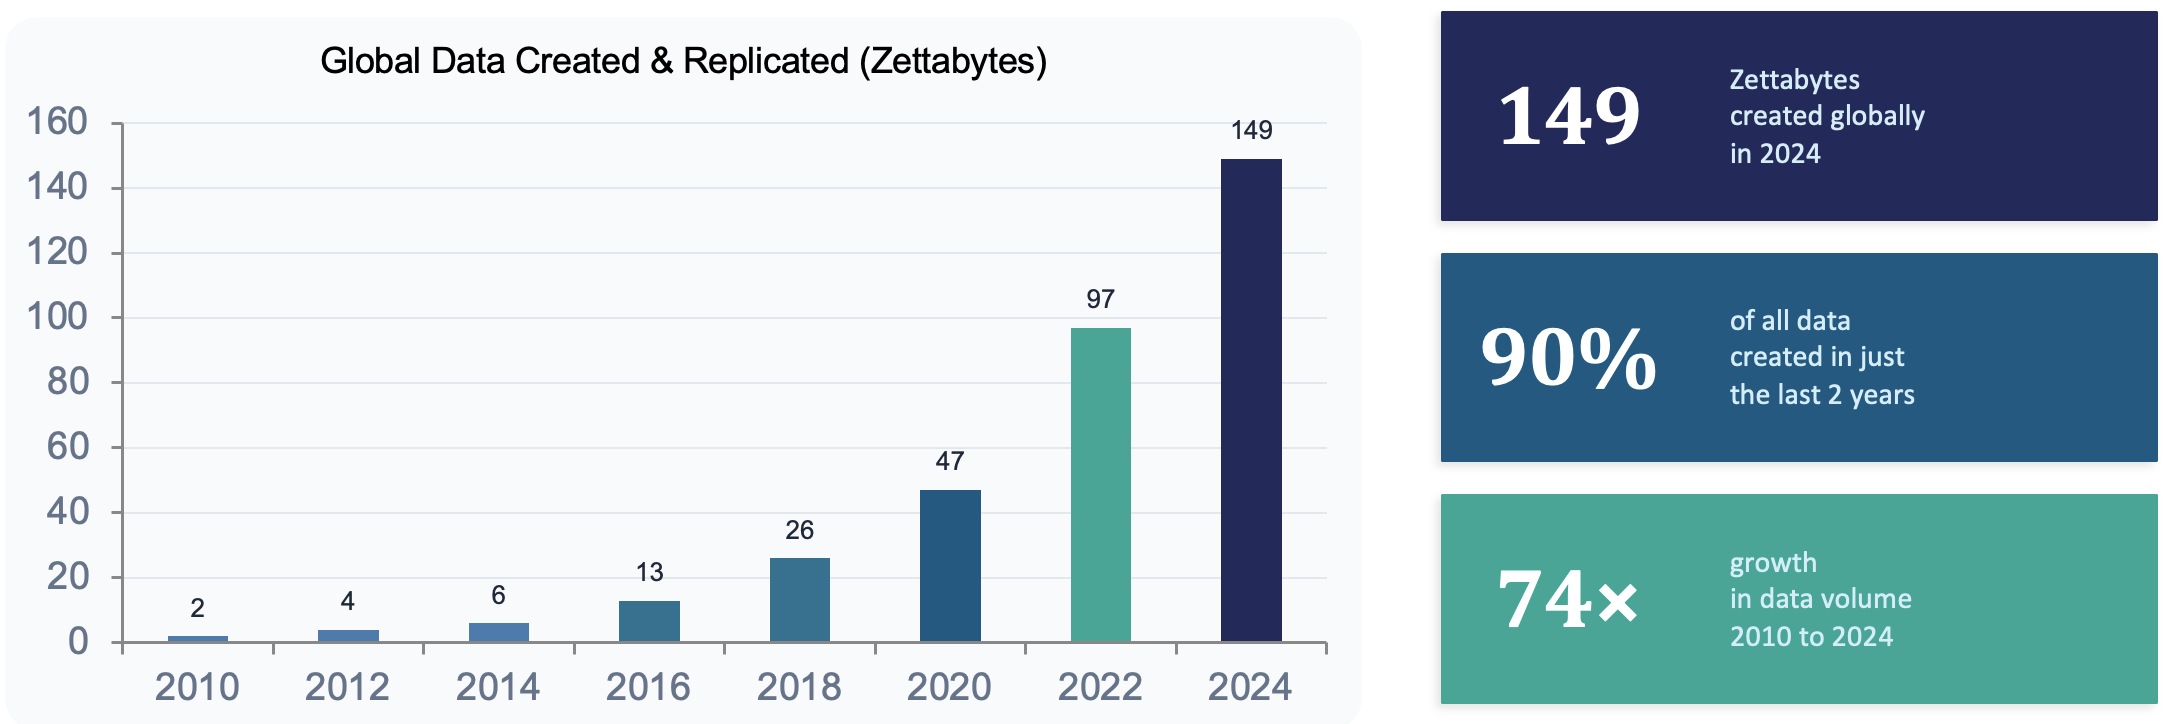
\includegraphics[width=0.85\linewidth]{slike/02/02-01.png}
    \caption{Визуелизација као аналитички механизам за управљање размером и сложеношћу окружења великих података (енг. big data)}
    \label{fig:02-1}
\end{figure}

У овом окружењу визуелизација постаје незаменљива за управљање размером и сложеношћу. Приступи визуелне аналитике комбинују технике аутоматизоване обраде података са интерактивним визуелним интерфејсима, омогућавајући корисницима да се крећу кроз велике скупове података уз очување свести о контексту (Keim et al., 2008). Ефективни визуелни прикази омогућавају аналитичарима да идентификују структуре високог нивоа пре него што се спусте на детаље, подржавајући принципе прегледа и детаља на захтев. Сходно томе, визуелизација није само слој презентације већ неопходан аналитички механизам за суочавање са савременим екосистемима података.

\subsubsection{Ланац вредности информација}
Визуелизација игра критичну улогу дуж читавог ланца вредности информација, који се може концептуализовати као кретање од података ка информацији, увиду и, коначно, одлуци. Сирови подаци састоје се од необрађених опажања која немају инхерентно значење без тумачења. Кроз аналитичку обраду и визуелизацију, подаци се трансформишу у информацију откривањем структуре, контекста и односа (Davenport \& Harris, 2007).

Увиди настају када доносиоци одлука тумаче визуелизовану информацију у оквиру специфичног доменског контекста, комбинујући аналитичке налазе са претходним знањем и искуством. Визуелизација олакшава овај процес тако што експлицитно приказује узрочне односе, трендове и аномалије, чиме подржава осмишљавање и расуђивање. Коначно, информисане одлуке доносе се када су увиди усклађени са организационим циљевима и ограничењима. Лоше осмишљене визуелизације могу искривити перцепцију и довести до погрешних закључака, док добро осмишљене визуелизације повећавају транспарентност, поверење и квалитет одлучивања (Knaflic, 2015).

Овај низ је лакше разумети ако се прати један исти пословни случај кроз све фазе. 

\textbf{\textit{Пример:}} Размотримо малопродајни ланац који бележи сваку продају по продавници, артиклу и датуму. На нивоу података, систем садржи велики број појединачних редова: 12. март, продавница 17, јогурт, 24 комада, цена 89 динара. Тај ред је чињеница, али још увек не и нешто што директно подржава управљачко расуђивање. Када се такви редови агрегирају по недељи, продавници и категорији производа, појављује се информација: продаја млечних производа у градским продавницама северног региона опала је 12\% у односу на исти период прошле године.

Увид настаје тек када се тој информацији дода контекст. Ако временска серија покаже да пад почиње тачно у недељи у којој је промењен распоред снабдевања, а поређење по продавницама открије да је проблем најјачи у објектима са најређим испорукама, онда је могуће формулисати смислено тумачење: пад продаје вероватно није последица слабије тражње, већ лошије расположивости робе на полици. Одлука је последњи корак: менаџер може да повећа учесталост испорука за критичне продавнице, привремено појача праћење залиха и после две недеље процени да ли је интервенција дала резултат. Тако се види да вредност не настаје у тренутку прикупљања података, већ у прелазу од евиденције ка тумачењу и од тумачења ка деловању.

\subsubsection{Експлораторна и експланаторна визуелизација}
Кључна разлика у пракси визуелизације јесте она између експлораторне и експланаторне визуелизације. 

\textbf{\textit{Експлораторна визуелизација}} се првенствено користи у раним фазама анализе података, када је циљ разумети податке, генерисати хипотезе и идентификовати обрасце без унапред дефинисаних очекивања. Ове визуелизације су често интерактивне, флексибилне и усмерене на аналитичара, с нагласком на брзину, итерацију и откривање (Tukey, 1977; Munzner, 2014).

Насупрот томе, \textbf{\textit{експланаторна визуелизација}} је осмишљена да комуницира специфичне налазе или поруке публици, често као део извештаја, контролних табли или презентација. Примарни циљ је јасноћа и уверљивост, а не откривање. Експланаторне визуелизације обично користе пажљиво одабрана кодирања, анотације и наративну структуру како би усмериле тумачење и смањиле двосмисленост (Few, 2012; Knaflic, 2015).

За ефективно доношење одлука, оба облика су неопходна и комплементарна. Експлораторна визуелизација подржава аналитичку ригорозност и генерисање увида, док експланаторна визуелизација обезбеђује да се увиди тачно и уверљиво комуницирају заинтересованим странама. Зрела аналитичка пракса интегрише оба приступа у оквиру кохерентног оквира анализе података и подршке одлучивању.

Најједноставније речено, експлораторна визуелизација служи да аналитичар открије шта се у подацима дешава. Он испробава различите приказе, филтере и поређења, тражи образац и тек онда прецизније формулише закључак. Експланаторна визуелизација долази после тога: њен циљ није откривање, већ јасно саопштавање већ уоченог налаза. На пример, аналитичар може најпре интерактивно истраживати продају по ценама и регионима, а затим направити један једноставан графикон који менаџеру јасно показује где је дошло до пада прихода. Зато је практично правило једноставно: експлораторна визуелизација помаже да нешто откријемо, а експланаторна да то што смо открили јасно објаснимо.

\subsection{Типови података}
Типови података диктирају начин њихове анализе и приказа. Типови података могу се широко класификовати према мерним скалама (категорички, ординални, интервални, размерни) и структурним карактеристикама (временски, просторни, хијерархијски и мрежни подаци). Ове класификације су комплементарне и често коегзистирају у сложеним скуповима података из стварног света (Knaflic, 2020).

\subsubsection{Мерне скале}
Најутицајнији оквир за класификацију мерних скала јесте Stevens-ова (1946) подела на четири скале: номиналну, ординалну, интервалну и размерну. 

\textbf{\textit{Категорички (номинални)}} подаци представљају квалитативне атрибуте чије вредности одговарају различитим, неуређеним категоријама. Операције над категоричким подацима ограничене су на поређења једнакости и неједнакости, а смислене нумеричке операције као што су сабирање или израчунавање просека нису дефинисане (Stevens, 1946).

Примери укључују: 

\begin{itemize}
  \item Пол, државу пребивалишта, категорију производа или тип дефекта у производњи. 
  \item \textbf{\textit{Крвну групу}} (\texttt{A}, \texttt{B}, \texttt{AB}, \texttt{0}) — категоричка је јер свака вредност означава различиту класу, али међу њима не постоји природан редослед.
  \item \textbf{\textit{Боју аутомобила}} (\texttt{црвена}, \texttt{плава}, \texttt{сива}, \texttt{црна}) — категоричка је јер су вредности само ознаке група, а не количине које се могу смислено поредити аритметички.
  \item \textbf{\textit{Студијске програме}} (\texttt{информациони системи и технологије}, \texttt{менаџмент и организација}) — категорички зато што означава припадност једној од више дискретних група, без имплицитног ранга међу њима.
  \item \textbf{\textit{Типове плаћања}} (\texttt{готовина}, \texttt{картица}, \texttt{мобилно плаћање}) — категорички јер описује начин извршења трансакције, а не мерљиву величину.
  \item \textbf{\textit{Оперативне системе}} (\texttt{Windows}, \texttt{Linux}, \texttt{macOS}) — категорички јер вредности представљају различите класе софтверских платформи, а не нивое исте нумеричке особине.
\end{itemize}
Заједничко свим овим примерима јесте да вредност променљиве одговара одговору на питање „којој категорији нешто припада?”, а не „колико нечега има?” или „које је место у поретку?”. Управо зато су дозвољена поређења типа „исто/различито”, док операције као што су сабирање, одузимање или просек немају интерпретативни смисао.

У напредној аналитици, категоричке променљиве се обично трансформишу техникама кодирања као што су јединично кодирање (енг. \textit{one-hot encoding}), циљно кодирање (енг. \textit{target encoding}) или угнежђене репрезентације (енг. \textit{embeddings}), у зависности од контекста моделовања. Неправилно третирање категоричких података — као што је наметање вештачког редоследа — може довести до пристрасних модела и обмањујућих тумачења (James et al., 2021).

\textbf{\textit{Ординални подаци}} поседују природан поредак међу категоријама, али растојања између категорија нису експлицитно дефинисана. То значи да ординални подаци омогућавају операције рангирања, али уз јаку претпоставку да су разлике између категорија једнаке. Типичан пример ординалног податка је успех у школи: Одличан, Врло добар, Добар, Довољан, Недовољан. Поредак ових категорија је јасан: Одличан > Врло добар > Добар > Довољан > Недовољан, међутим не постоји квантитативна информација о величини разлика између категорија (Одличан је једнако бољи од Врло доброг, као што је и Добар бољи од Довољног). Додатно, коришћењем ординалних података уместо нумеричких губи се део информација које иначе могу бити доступне. Узмимо за пример два ученика која су имала просечну оцену у средњој школи 4,51 и 5,00 респективно. Ако се ови ученици посматрају кроз ординалну скалу, оба ученика имају \textbf{\textit{Одличан }}успех и међу њима нема разлике по успеху у средњој школи. Међутим, ако их посматрамо кроз континуалну скалу вредности, други ученик је бољи од првог. 

Упркос ограничености ординалних променљивих оне се често третирају као нумеричке (континуалне), нарочито у регресионим моделима. Овакав третман номиналних података је често оправдан, нарочито у ситуацијама када није могуће прикупити (измерити) прецизне податке (нпр. доступан је само номинални успех у школи или описни квалитет производа). У неким ситуацијама је чак и пожељно користити номиналне податке зато што занемарују мање разлике које доносиоцима одлука нису битне (нпр. просек 4.82 и 4.85). Ипак при коришћењу ординалних уместо нумеричких података, претпоставке морају бити експлицитно оправдане или замењене моделима специфичним за ординалне податке, као што је ординална логистичка регресија (Agresti, 2010).

Типични примери ординалних података укључују: 

\begin{itemize}
  \item Одговоре у анкетама са Ликертовом скалом (нпр. од „уопште се не слажем” до „у потпуности се слажем”), нивое задовољства купаца или кредитне рејтинге.
  \item \textbf{\textit{Ниво образовања}} (\texttt{основно}, \texttt{средње}, \texttt{високо}, \texttt{мастер}, \texttt{докторске студије}) — јер постоји јасан редослед нивоа, али разлике између њих нису једнаке у квантитативном смислу.
  \item \textbf{\textit{Приоритет захтева}} (\texttt{низак}, \texttt{средњи}, \texttt{висок}, \texttt{критичан}) — јер категорије могу да се рангирају по важности, али се не може рећи да је, на пример, \texttt{критичан} приоритет нумерички „два пута већи” од \texttt{средњег}.
\end{itemize}
\textbf{\textit{Интервални подаци}} су нумерички подаци са једнаким размацима између вредности, али без стварне нулте тачке. Примери укључују:

\begin{itemize}
  \item \textbf{\textit{Температуру}} мерену у Целзијусовим или Фаренхајтовим степенима. Разлике између вредности су смислене, али размери нису (нпр. 20°C није „два пута топлије” од 10°C).
  \item \textbf{\textit{Календарску годину}} (\texttt{1990}, \texttt{2000}, \texttt{2025}), јер је разлика између година смислена и једнака, али не постоји апсолутна нулта година која би омогућила тумачење размера. Зато нема смисла рећи да је 2000. година „два пута већа” од 1000. године.
  \item \textbf{\textit{Време на сату у току дана}} (нпр. \texttt{08:00}, \texttt{12:00}, \texttt{16:00}), јер су временски размаци једнаки и могу се смислено поредити као разлике, али почетна тачка је конвенционална, а не природна нула. Због тога није исправно тврдити да је 16:00 „два пута више” од 08:00.
\end{itemize}

У статистичком моделовању, интервални подаци подржавају широк опсег операција, укључујући линеарне трансформације и параметарску инференцију, под условом да су дистрибутивне претпоставке испуњене. Међутим, тумачење коефицијената модела мора уважавати одсуство апсолутне нуле (Stevens, 1946).

\textbf{\textit{Размерни (рацио) подаци}} проширују интервалне податке укључивањем нулте тачке, што омогућава тумачење и разлика и размера. Заједничка особина свих размерних података јесте постојање стварне нуле, која не представља произвољан почетак скале већ одсуство мерене појаве. Управо зато су код ове скале дозвољене и аритметичке операције над разликама и тумачења односа типа „два пута више” или „упола мање”, што код интервалних података није случај. Примери укључују:

\begin{itemize}
  \item Тежину, приход, обим продаје, трајање времена, растојање.
  \item \textbf{\textit{Број продатих производа}} (\texttt{0}, \texttt{5}, \texttt{10}, \texttt{20}) — јер нула значи потпуно одсуство продаје, а однос вредности има смисла, па се може рећи да је 20 продатих производа два пута више од 10.
  \item Старост особе (мерена у годинама), јер постоји природна нулта тачка на рођењу, а и разлике и размере имају интерпретативни смисао. На пример, разлика између 20 и 30 година је 10 година, а 30 година јесте један и по пут више од 20 година.
  \item Потрошња електричне енергије у киловат-часовима, јер вредност \textbf{\textit{\texttt{0}}} означава да потрошње нема, а вредности се могу смислено поредити и по разлици и по односу.
\end{itemize}
Променљиве размерне скале су најфлексибилније у аналитичким контекстима и уобичајено се користе у оптимизацији, регресији, кластеровању и предиктивном моделовању. Многи алгоритми машинског учења имплицитно претпостављају улазне податке на размерној скали, посебно када користе метрике засноване на растојању (Hastie et al., 2009).

\subsubsection{Структурни типови података}
Поред мерних скала из §2.1.2.1, подаци се могу разликовати и према својој структури, односно према начину на који су опажања међусобно организована и повезана. Мерна скала описује једну променљиву, док структурни тип података описује односе међу опажањима (мерењима): да ли су распоређена кроз време, везана за простор, угнежђена у нивое или повезана мрежом односа. Управо ти односи утичу на избор аналитичких метода и начина визуелизације.

У литератури се најчешће издвајају четири структурна типа података: \textbf{\textit{временски}}, \textbf{\textit{просторни}}, \textbf{\textit{хијерархијски}} и \textbf{\textit{мрежни}}. Заједничка карактеристика ових типова података јесте да опажања нису потпуно независна једна од других. Због тога класичне методе које полазе од претпоставке независности често нису довољне, па је неопходно користити приступе који експлицитно узимају у обзир временску, просторну, хијерархијску или мрежну повезаност.

\textbf{\textit{Временски подаци}}. Временски подаци обухватају опажања индексирана временом и централни су у областима као што су финансије, економија, аналитика сензора и управљање операцијама. Примери укључују временске серије цена акција, серверске логове или физиолошка мерења.

Временски подаци уводе изазове као што су аутокорелација, сезоналност, померај концепта и нестационарност и захтевају посебне методе за визуализацију и напредну аналитику.

Практичан пример је дневна продаја супермаркета током године. Овде је природна визуелизација линијски графикон, јер јасно показује тренд, сезонске осцилације и нагле прекиде, као што су празнични нагли успони или падови изазвани несташицом робе. Ако је циљ поређење више серија, на пример продаје по категоријама производа, линијски графикон и мали умножени прикази (енг. \textbf{\textit{small multiples}}) често су читљивији од једне претрпане табеле.

Напредна анализа захтева специјализоване методе, укључујући декомпозицију временских серија и рекурентне неуронске мреже (Box, Jenkins, Reinsel, \& Ljung, 2015). Игнорисање временске структуре често доводи до нетачних предвиђања и претерано оптимистичне процене квалитета модела.

\textbf{\textit{Просторни подаци}}. Просторни подаци описују опажања повезана са физичким локацијама у дводимензионалном или тродимензионалном простору. Примери укључују географске координате, сателитске снимке, податке о урбаној инфраструктури и мерења животне средине. У пракси се они често чувају као геометријски објекти које софтвер уме да прочита и прикаже на карти, на пример као тачке, линије и полигоне. Полигон може представљати границу општине, катастарске парцеле, продајне зоне или државе, док се у форматима као што су \textit{GeoJSON}, \textit{Shapefile} или \textit{WKT} ти облици записују тако да их алати за визуелизацију, GIS системи и BI платформе могу директно учитати и исцртати.

Просторни подаци често имају једноставну особину: оно што је близу у простору често је сличније него оно што је далеко. Зато се просторни подаци не могу увек тумачити као скуп потпуно независних тачака. У напреднијим анализама постоје посебне методе за рад са таквим зависностима, али је за уводно разумевање довољно запамтити да простор сам по себи носи део значења података (Cressie, 1993).

Практичан пример је анализа стопе незапослености по општинама. Ако је циљ да се уочи географска концентрација проблема, хороплет карта је прикладна визуелизација, јер омогућава да се стопе упореде у просторном контексту. Ако је, међутим, циљ прецизно рангирање општина, карту је пожељно допунити стубичастим графиконом, јер сама карта није најбољи алат за тачно поређење вредности.

\textbf{\textit{Хијерархијски подаци}}. Хијерархијски (вишенивоски) подаци настају када су опажања угнежђена у јединице вишег нивоа, као што су студенти унутар одељења, запослени унутар сектора или поновљена мерења унутар појединаца.

Код оваквих података важно је да не посматрамо свако опажање као потпуно изоловано. Студенти из исте групе, на пример, често су сличнији једни другима него студентима из друге групе. Зато анализа мора да узме у обзир и појединца и ниво изнад њега. У напреднијим курсевима то се решава посебним моделима, али је овде најважнија сама интуиција да структура група мења начин тумачења података (Gelman \& Hill, 2007).

Практичан пример је образовни систем у коме су студенти угнежђени у групе, групе у студијске програме, а програми у факултете. Ако анализирамо пролазност на испиту, резултат једног студента није одређен само његовим индивидуалним карактеристикама, већ и квалитетом наставе у групи, структуром програма и факултетским окружењем. Зато је корисно користити визуелизације које приказују и структуру и величину, на пример treemap за приказ удела студената по факултету, програму и години студија, или дендрограм када је важније показати чист однос надређености и подређености. Избор визуелизације зависи од питања: да ли желимо да разумемо само структуру гранања или и расподелу величина унутар сваког нивоа.

\textbf{\textit{Мрежни подаци}}. Мрежни подаци представљају ентитете (чворове) и њихове односе (ивице), као што су друштвене мреже, цитатне мреже, комуникациони графови или ланци снабдевања.

За разлику од обичних табела, овде није најважније само шта је сваки чвор појединачно, већ како је повезан са другим чворовима. Зато се код мрежних података често гледа ко је у средишту мреже, где постоје групе повезаних чворова и где настају уска грла. Постоје и веома напредне методе за анализу таквих мрежа, али је за основни ниво најважније разумети да је сама структура веза главни носилац информације (Newman, 2018).

Пословни пример је ланац снабдевања у коме су добављачи, дистрибутивни центри и продавнице повезани токовима робе. Ако један добављач касни, последице се не шире кроз фиксну хијерархију, већ кроз мрежу зависности: један центар може снабдевати више продавница, а више добављача може делити исто транспортно чвориште. Зато је природна визуелизација мрежни дијаграм, у коме величина чвора може приказивати обим испорука, а дебљина везе интензитет тока. Када је мрежа превише густа, матрица повезаности је често прегледнија, јер смањује визуелно преклапање и јасније открива кластере, централне чворове и уска грла.

\subsection{Аналитички задаци}
Поред типова података за потребе креирања информативних визуализација потребно је разумевање аналитичких задатака које визуализације могу да решавају, тј. од питања на које је потребно добити одговор. У пракси се већина графикона користи за мали број понављајућих задатака, а избор графикона не треба да почиње питањем „шта лепо изгледа”, већ питањем „шта желимо да видимо у подацима”. У наредном тексту су описани типични аналитички проблеми које је могуће решавати различитим техникама визуелизације.

\textbf{\textit{Поређење међу групама}} одговара на једноставно питање: која је група већа, мања или успешнија од друге. То може бити поређење производа, региона, сегмената купаца или одељења. Ово је један од најчешћих задатака у пословној аналитици, јер велики број питања на крају гласи: „ко има више, мање или највише?”.

\textbf{\textit{Анализа тренда}} током времена одговара на питање како се нека вредност мења из дана у дан, из месеца у месец или из године у годину. Ту нас обично занима да ли нешто расте, опада, понавља се сезонски или нагло мења правац. Овај задатак је важан за праћење перформанси и за процену да ли је нека пословна одлука донела очекивани резултат.

\textbf{\textit{Корелација између променљивих}} бави се питањем да ли две величине иду заједно и како. На пример, да ли већа цена прати мању продају, да ли више сати учења прати бољи резултат или да ли се веза мења у различитим групама. Овај задатак је важан јер често представља први корак ка дубљем објашњењу појаве.

\textbf{\textit{Расподела једне променљиве}} показује како су вредности распоређене, а не само колики је просек. Ту нас занима да ли су вредности збијене или распршене, да ли има много ниских или високих случајева и да ли постоје издвојене вредности. Ово је важно јер исти просек може сакрити веома различите ситуације у позадини.

\textbf{\textit{Анализа односа дела и целине}} испитује како се укупна количина разлаже на своје саставне компоненте и како се релативни удели тих компоненти међусобно пореде или мењају током времена. Основни проблем је проблем композиције, а не величине: не колико је сваки део велик у апсолутном смислу, већ који део целине представља и да ли се тај удео мења. Овај задатак се јавља кад год се разматрају буџети, тржишни удели, алокације портфолија или структура прихода, и захтева да компоненте буду и међусобно искључиве и заједно исцрпне да би анализа имала смисла.

\textbf{\textit{Географски обрасци}} односе се на варијације међу просторним јединицама — државама, регионима, поштанским бројевима или произвољним захватним подручјима. Аналитички проблем превазилази једноставно приказивање локација и обухвата питања просторне аутокорелације, ефеката суседства и зависности исхода од географског контекста. Просторна анализа је суштинска свуда где су одлуке ограничене физичком удаљеношћу, регулаторним границама или дистрибутивним мрежама, и мора се третирати пажљиво јер избор јединице агрегације може значајно променити донете закључке.

\textbf{\textit{Матрична или унакрсно-табеларна анализа}} представља природан задатак када се укрштају две категоријалне димензије и квантитативна мера се пријављује за сваку комбинацију. Проблем је открити ћелије неуобичајене концентрације, идентификовати редове или колоне које се систематски разликују од осталих и очитати ефекте интеракције између две класификујуће променљиве. Овај задатак лежи у основи cohort анализа, анализа профитабилности по каналима и производима и студија сегментације, и елегантно се скалира и на ординалне и на номиналне класификације, под условом да кардиналност сваке димензије остане визуелно прегледна.

Ових седам задатака ретко се јавља у изолацији. Типична аналитичка истрага повезује неколико њих заједно — пореди категорије унутар временског тренда, испитује расподелу мере по географским јединицама или разлаже структуру дела и целине кроз унакрсно-табеларне сегменте. Јасно навођење који задатак или комбинацију задатака визуелизација треба да подржи представља предуслов за пресликавање аналитичке намере у визуелну форму, чему је посвећен следећи одељак.

\subsection{Типови и избор техника визуализације}
Квалитет визуелизације се не одређује њеном упадљивошћу, већ усклађеношћу са подацима и постављеним питањем (задатком). Графикон се сматра добрим ако је њиме јасно приказано оно што треба да буде анализирано. Избор визуелне форме стога није ствар естетике, већ усклађивања расположивих података, циља анализе и приказа којим се то најјасније преноси.

Основни принцип је једноставан: бирају се прикази који се лако читају. Положај и дужина се, на пример, прецизније пореде него боја или површина. У наредном тексту ће бити описани основни типови графикона и њихова веза са типовима података и задацима које решавају.

\subsubsection{Поређење група и стубичасти графикони}
Када је примарни задатак поређење величина међу дискретним категоријама, користи се стубичасти графикон као перцептивно ефикасно решење. За креирање основног стубичастог графикона, неопходно је коришћење једне категоричке и једне квантитативне променљиве (која је најчешће агрегирана збиром, средњом вредношћу или бројем). Свака категорија се пресликава на посебан положај дуж осе, а квантитативна вредност се кодира дужином стубца.

\textbf{\textit{Пример:}} размотримо универзитетског администратора који пореди просечне резултате испита по испитима (Слика~\ref{fig:02-2}). Називи испита представљају категоричку променљиву, док је просечан резултат квантитативан. Стубичасти графикон омогућава непосредно поређење, јер се разлике у дужини стубаца лако уочавају. Емпиријске студије графичке перцепције потврђују да кодирања заснована на дужини подржавају тачнија поређења него алтернативе засноване на површини или углу (Cleveland \& McGill, 1984).

\begin{figure}[h]
    \centering
    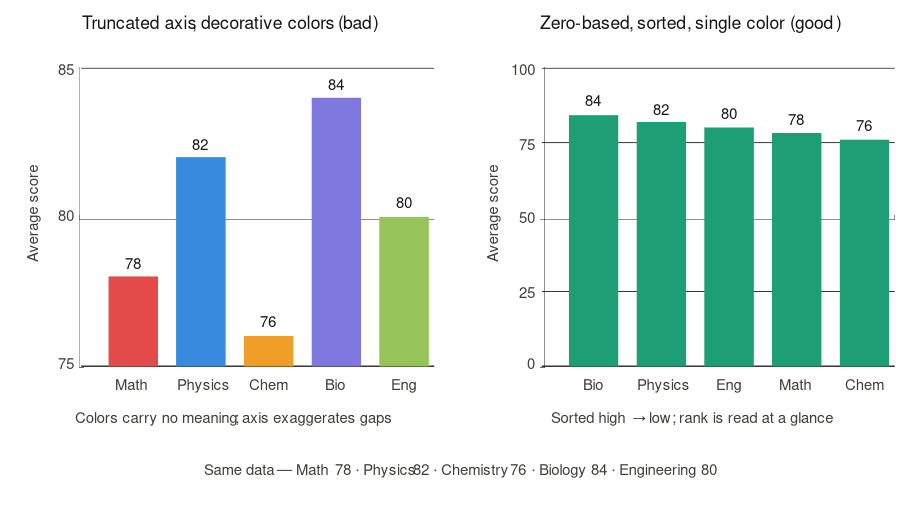
\includegraphics[width=0.85\linewidth]{slike/02/02-05.png}
    \caption{Стубичасти графикон просечних резултата испита по одељењима}
    \label{fig:02-2}
\end{figure}

Упркос својој једноставности, стубичасти графикони се често погрешно користе. Уобичајене грешке укључују скраћивање вертикалне осе, што преувеличава разлике, или примену стубичастих графикона на континуалне променљиве где би другачије визуелизације биле прикладније.

На Слици 2 се може видети пример лоше (лево) и добро (десно) дефинисаног стубичастог графа. На левом графикону је оса скраћена, чиме су разлике међу одељењима преувеличане, а ступци су поређани абецедно. Додатно, коришћене су различите боје (за сваки стубац) које не енкодирају никакве вредности (коришћене су само због естетике а не приказују податке). Због оваквог дизајна графа, читаоцу је потребно доста времена да добије одговоре на нека питања нпр: 

\begin{itemize}
  \item Који предмет има најбољу, а који најлошију просечну оцену?
  \item Која је разлика у поенима између најбољег и најлошије оцене на предметима?
\end{itemize}
На десном графикону оса почиње од нуле, а ступци су поређани по вредности, а боја свих стубаца је иста. На овај начин је поређење између предмета веродостојно приказано и омогућава једноставну и брзу анализу.

Ефективност стубичастог графикона зависи од малог броја дизајнерских одлука чија логика директно следи из перцептивне основе кодирања. Пошто дужина стубца носи квантитативно значење, сваки поступак који скреће пажњу са опажене дужине — скраћена основа, 3D аспеката (енг. \textbf{\textit{facet}}), почетак различит од нуле — искривљује и поређење које се од читаоца тражи. Додатно, редослед приказа значајно утиче на једноставност разумевања визуелизације: алфабетски редослед је прикладан само када сами називи носе аналитичку релевантност, док рангирање по вредности у први план ставља поређење које графикон и треба да подржи. Правила која следе консолидују ова разматрања у радну контролну листу:

\begin{itemize}
  \item Оса се започиње од нуле (величина се кодира дужином).
  \item Ступци се ређају по вредности (не абецедно), осим ако је редослед значајан.
  \item Хоризонтални ступци се користе за дугачке ознаке категорија.
  \item 3D приказ се избегава — њиме се искривљује перцепција дужине.
  \item Боја се користи само за кодирање друге променљиве, а не ради декорације.
\end{itemize}

\subsubsection{Анализа односа дела и целине}
Када аналитички задатак налаже приказ укупне вредности која разлаже на своје саставне компоненте, подаци се састоје од једне категоријалне променљиве чији нивои деле целину и квантитативне мере — типично збира или удела. Кружни графикон је најпознатији визуелни облик за овај задатак, кодирајући сваку компоненту као угаони исечак круга чија укупна површина представља целину. У пракси се овај графикон често назива и питичасти графикон, по узору на енглески термин \textbf{\textit{pie chart}}, који дословно значи „графикон у облику пите”. Графикон се интуитивно чита као композиција, а не као скуп независних величина, што представља његову главну аналитичку предност када су удели променљива од интереса.

\textbf{\textit{Пример:}} руководилац који прегледа структуру укупног прихода по линијама производа може користити кружни графикон да на први поглед прикаже које линије доминирају структуром, а које су маргиналне. Визуелни нагласак пада на релативне уделе, а не на апсолутне вредности, што је прикладно када се аналитичко питање односи на пропорционалност. Емпиријске студије графичке перцепције су ипак показале да су процене угла и површине знатно мање тачне од процена дужине дуж заједничке скале (Cleveland \& McGill, 1984), те је кружне графиконе најбоље резервисати за случајеве у којима је категорија мало, разлике између удела велике, а аналитичка порука квалитативна, а не квантитативна.

Када је потребно прецизно поређење удела, или када је број компоненти велики, пожељнији су алтернативни визуелни облици. Наслагани стубичасти графикони чувају тумачење дела и целине, а истовремено омогућавају тачније поређење засновано на дужини, и нарочито су ефективни када више целина треба поредити једну поред друге, као у структури прихода по регионима или кварталима.

\begin{figure}[h]
    \centering
    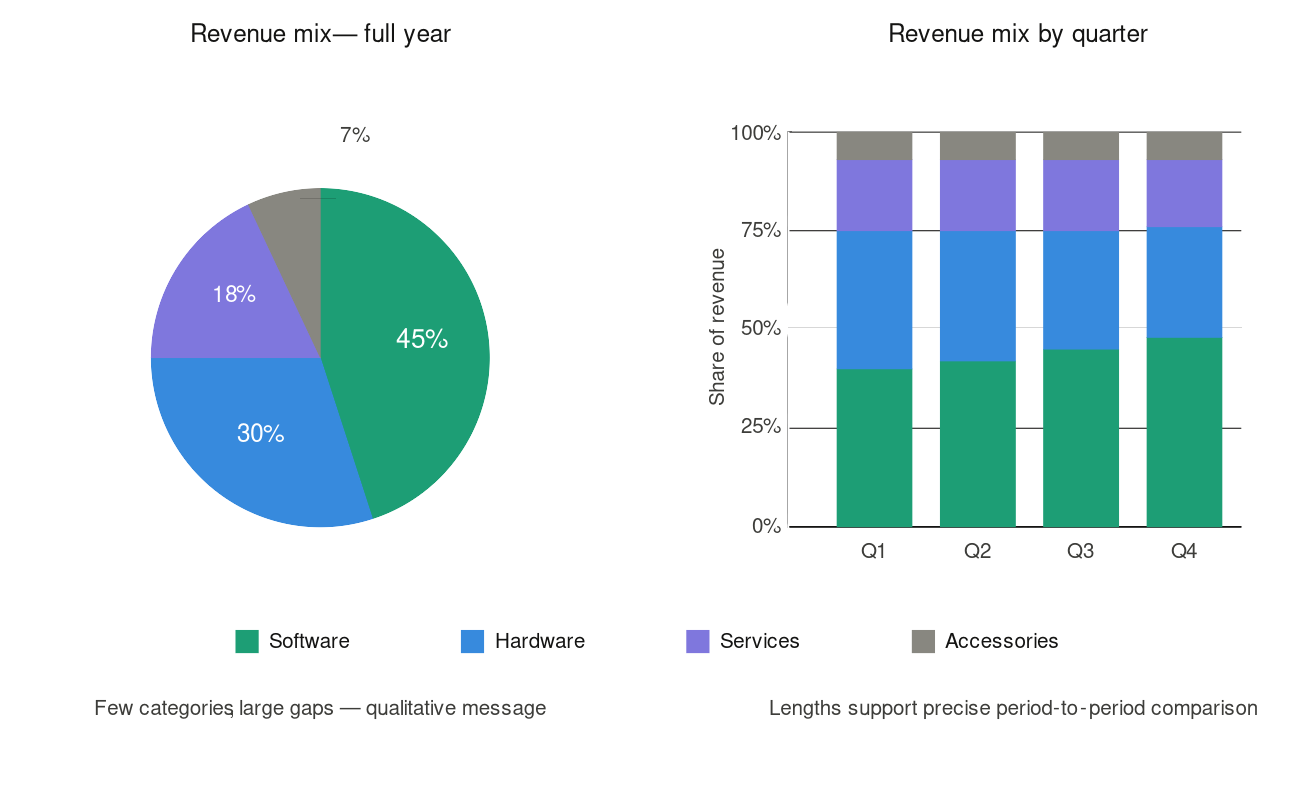
\includegraphics[width=0.85\linewidth]{slike/02/02-15.png}
    \caption{Кружни графикон и наслагани стубичасти графикон структуре прихода на нивоу целе године}
    \label{fig:02-3}
\end{figure}

Кружни графикон приказује поделу годишњег прихода — \textit{Software} доминира са 45\%, \textit{Accessories} је маргиналан са 7\% — што је типичан случај „мало категорија, велике разлике” у коме се кружни графикон тренутно чита (Слика~\ref{fig:02-3} лево). Наслагани стубичасти графикон десно узима исте четири линије производа и приказује њихов састав кроз Q1–Q4, тако да постепени раст \textit{Software}-а (40\% → 48\%) и компензациони пад \textit{Hardware}-а (35\% → 28\%) постају прецизно читљиви као разлике у дужини дуж заједничке основе (Слика~\ref{fig:02-3} десно).

\textbf{\textit{Мапе стабла}} (енг. \textit{treemap}) проширују исту логику на хијерархијске композиције, кодирајући угнежђене компоненте површином и омогућавајући смештај десетина категорија које би преоптеретиле кружни графикон. Уобичајене замке у свим приказима дела и целине укључују употребу тродимензионалних ефеката који искривљују перцепцију удела, укључивање категорија које заједно не исцрпљују целину и примену ових облика на податке који по својој природи нису истински композициони.

\begin{figure}[h]
    \centering
    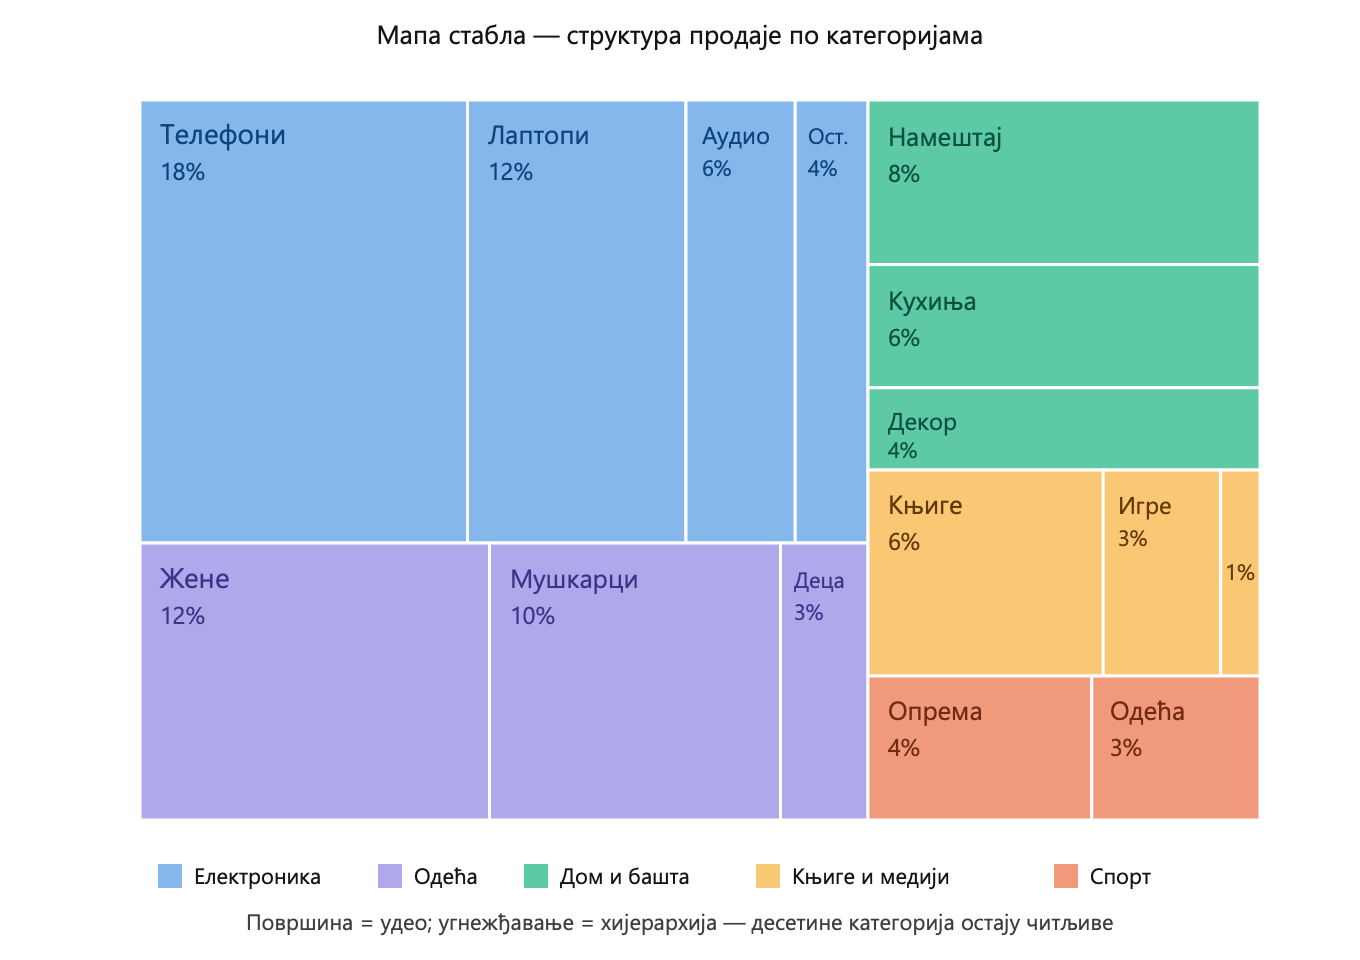
\includegraphics[width=0.85\linewidth]{slike/02/02-07.png}
    \caption{Мапа стабла}
    \label{fig:02-4}
\end{figure}

Мапа стабла приказује четрнаест подкатегорија продаје груписаних у пет главних категорија, при чему је површина сваког правоугаоника пропорционална уделу у укупној продаји. Електроника доминира са 40\% (Телефони сами носе 18\%), док мање категорије попут Музике (1\%) и даље остају видљиве — нешто што би на кружном графикону постало нечитљиво. Боја кодира главну категорију, а угнежђено распоређивање показује двослојну хијерархију без додатних осовина.

\subsubsection{Линијски и површински графикони}
Када су подаци индексирани временом, а аналитички циљ је идентификовати трендове, обрасце или временску промену, линијски графикони (енг. \textbf{\textit{Line charts}}) су најприкладнији визуелни облик. У овом случају, подаци се састоје од временске променљиве и квантитативне променљиве, при чему је време пресликано на хоризонтални положај (X-осу), а величина на вертикални положај (Y-осу).

Као илустративан пример, енергетски снабдевач који прати месечну потрошњу електричне енергије током више година може користити линијски графикон да открије сезонске флуктуације и дугорочни раст. Континуална природа линије појачава уређену структуру времена и омогућава посматрачима да уоче промене нагиба, које људи ефикасно тумаче као растуће или опадајуће трендове (Few, 2012). Линијски графикони постају проблематични када се примењују на неуређене категорије или када се истовремено прикаже превише линија, што доводи до визуелног нереда и интерпретативне двосмислености.

Близак сродник линијског графикона је површински графикон (енг. \textbf{\textit{Area chart}}), у коме је област између линије и хоризонталне осе попуњена како би се нагласила кумулативна величина, а не тренутна вредност. Површински графикони су погодни за комуницирање обима активности током времена — укупна продаја, укупна потрошња енергије, укупан улазни саобраћај — јер се попуњена површина чита као интеграл основне величине. Овај облик се природно проширује на наслагане површинске графиконе, који разлажу временски укупни износ на његове компонентне серије и комбинују тумачење дела и целине са временским, омогућавајући аналитичару да прати и еволуцију укупне величине и променљив састав њених делова. Површински графикони су ипак склони специфичним замкама: наслагане варијанте отежавају читање путање било које серије осим доње, јер свака горња серија лежи на флуктуирајућој основи, а преклапајући ненаслагани површински графикони заклањају појединачне серије услед оклузије. Зато су најделотворнији када је аналитички нагласак на агрегатној величини, а не на прецизном поређењу између компонентних серија.

\begin{figure}[h]
    \centering
    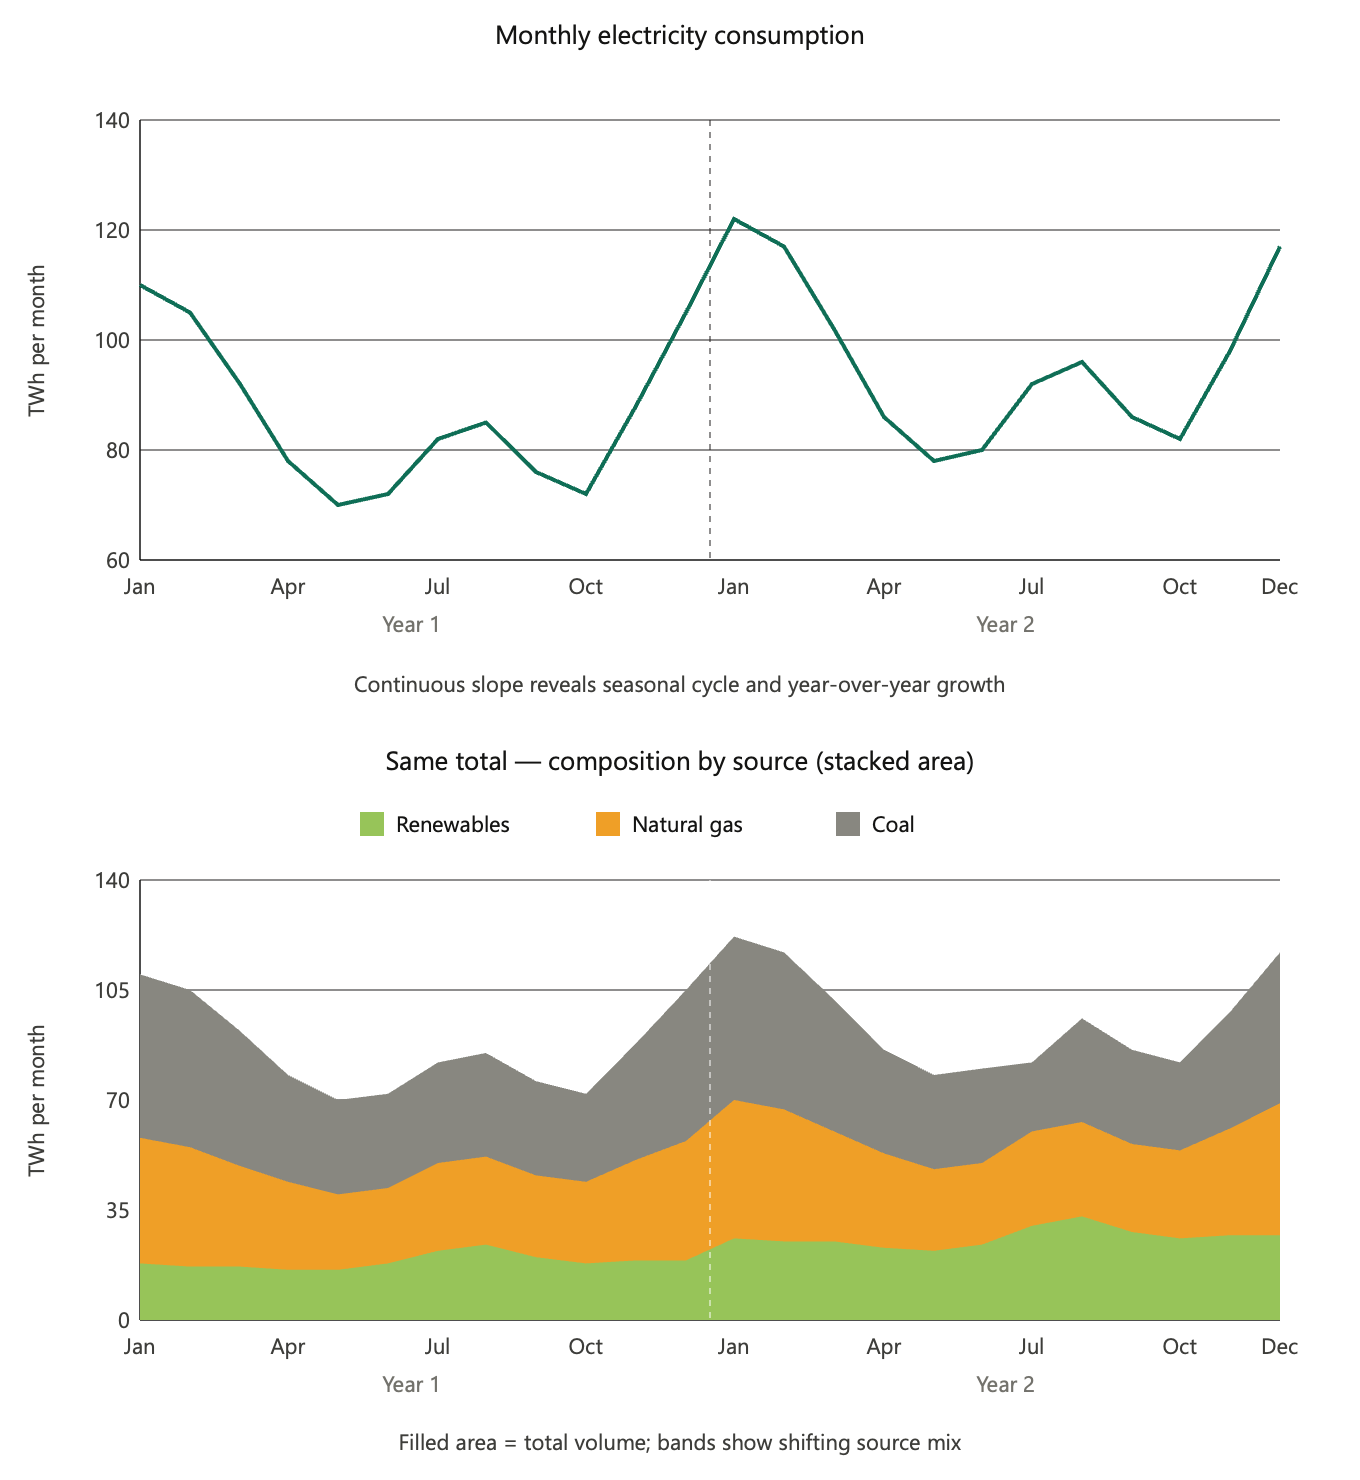
\includegraphics[width=0.85\linewidth]{slike/02/02-13.png}
    \caption{Линијски и површински графикон}
    \label{fig:02-5}
\end{figure}

Линијски графикон на врху приказује кретање укупне месечне потрошње електричне енергије кроз 24 месеца — кодирање нагибом чини сезонски циклус (зимски врхови у јануару, летњи падови у мају и јуну) и међугодишњи раст из прве у другу годину одмах читљивим као промене у смеру линије.

Површински графикон са слагањем испод приказује исте укупне вредности, али их разлаже на обновљиве изворе, природни гас и угаљ. Сада попуњене области преносе кумулативни обим — висина целог стека је укупна потрошња — док релативне дебљине трака показују да су обновљиви извори порасли (са око 18 на 30 TWh у зимским врховима), а да је учешће угља у истом периоду опало. То је двоструко читање које текст описује: временски тренд укупне вредности и промена у структури њених делова у једном кадру.

\subsubsection{Односи између променљивих}
Истраживање односа између нумеричких променљивих представља централни задатак у експлораторној анализи података, а „раштркани” дијаграми (енг. \textbf{\textit{Scatter plots}}) су посебно осмишљени за ту сврху. Раштркани дијаграм конструише се од две квантитативне променљиве, од којих је свака пресликана на једну од оса, док је свако опажање представљено као тачка у дводимензионалном простору.

Раштркани дијаграми могу бити обогаћени додатним кодирањима као што су боја или облик ради представљања категоричких груписања, али прекомерно украшавање може прикрити основну структуру података.

Читање раштрканог дијаграма почиње општим обликом „раштрканих” тачака. Ако се тачке у просеку подижу слева надесно, постоји позитивна корелација; ако се спуштају, корелација је негативна. Јачина везе не процењује се само по постојању нагиба, већ и по томе колико су тачке збијене око замишљеног тренда. Збијен и издужен облик указује на јаку повезаност (корелацију), док разливен облак указује на слабу. Овде је важно нагласити да раштркани дијаграм не служи само да покаже „има ли корелације”, већ и како је та повезаност обликована. Коначно, и када је образац јасан, мора се задржати основна методолошка опрезност: корелација није каузалност. Визуелизација открива да две променљиве иду заједно; она сама не доказује да једна узрокује другу.

Посебно је важно уочити нелинеарност. Многи односи у стварним подацима нису праволинијски: могу имати U-облик, праг након кога се промена убрзава, или ефекат засићења у коме даљи раст једне променљиве све мање прати раст друге. На пример, број сати учења и резултат на испиту могу бити позитивно повезани само до одређене тачке, после које додатно учење доноси све мањи добитак. Овакви закључци обично воде до додатних анализа и укључивања додатних променљивих (нпр. шта још утиче на коначну оцену: посета предавањима и вежбама, интеракција са наставним материјалима, концентрација приликом учења итд.). Управо зато визуелни преглед често открива нешто што једна једина корелациона мера не може да прикаже.

Раштркани дијаграм омогућава и уочавање кластера (група сличних података) и издвојених вредности. Кластери су важни јер могу указивати на постојање различитих подгрупа унутар истог скупа података, рецимо студената који редовно похађају наставу и оних који уче само пред испит. Издвојене вредности су подједнако значајне: оне могу бити грешке у уносу, али и случајеви од посебног аналитичког интереса. 

Раштркани дијаграм се често користи и за идентификацију екстремних вредности (енг. outliers) — тачака које значајно одступају од општег обрасца. Такве вредности се препознају као мали број изолованих тачака које су удаљене од главне масе података и подлежу додатној провери, јер могу указивати на грешку у мерењу, али и на ретке догађаје који носе важан аналитички сигнал.

\textbf{\textit{Пример:}} истраживач који испитује однос између времена проведеног у учењу и резултата на испиту може користити раштркани дијаграм да идентификује корелације, кластере сличног понашања или екстремне вредности (аутлајере). За разлику од агрегираних визуелизација, раштркани дијаграми чувају појединачна опажања, подржавајући генерисање хипотеза, а не њихову потврду (Tukey, 1977).

\begin{figure}[h]
    \centering
    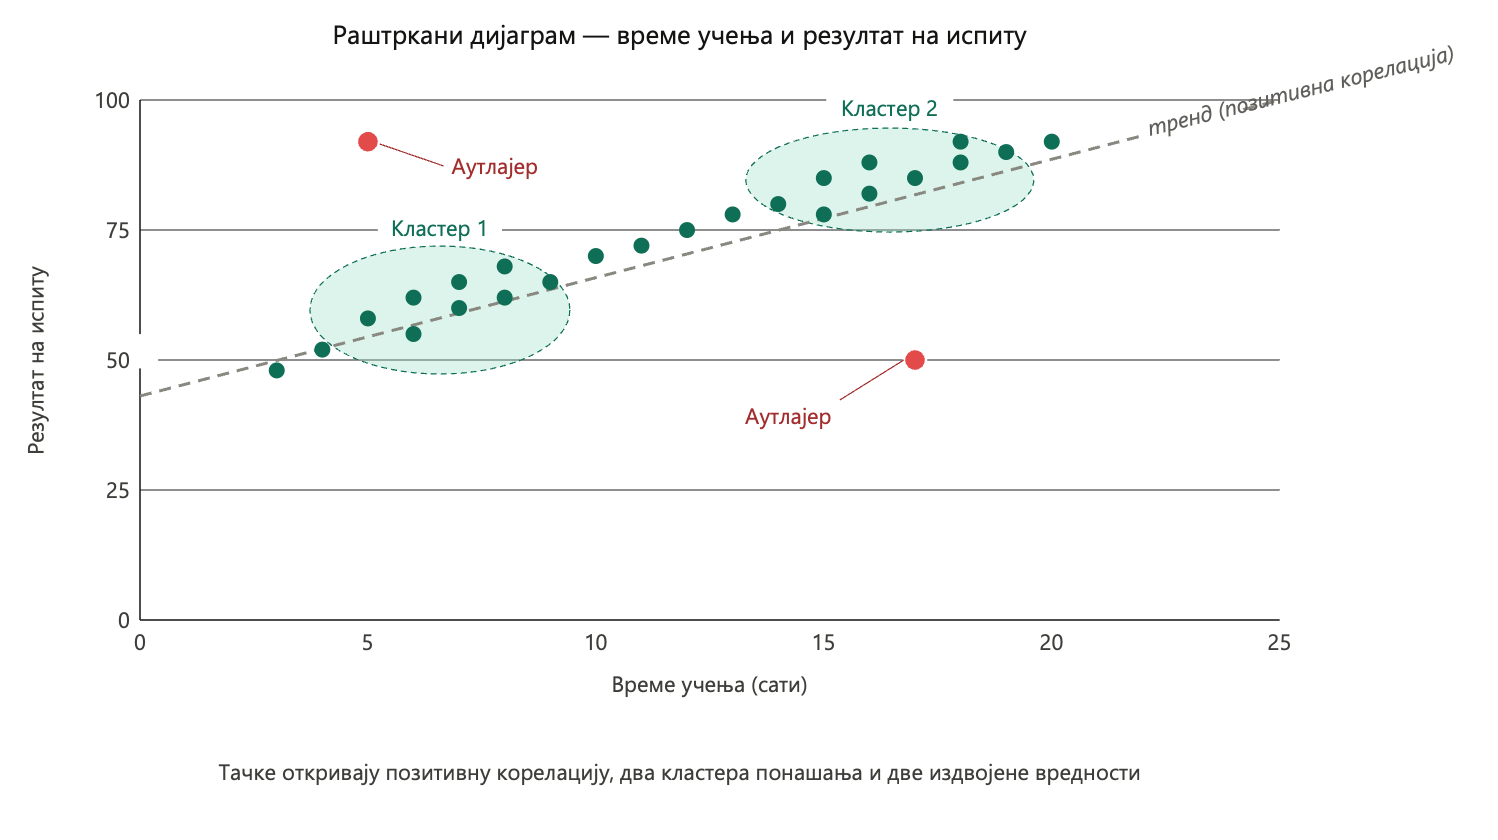
\includegraphics[width=0.85\linewidth]{slike/02/02-02.png}
    \caption{Раштркани дијаграм}
    \label{fig:02-6}
\end{figure}

Раштркани дијаграм истовремено показује сва три обрасца које текст наводи. Испрекидана сива линија тренда се пење с лева на десно — то је позитивна корелација између времена учења и резултата на испиту. Два светло осенчена овала истичу кластере сличног понашања: студенти са умереним учењем и умереним резултатима у доњем левом делу, и студенти са дуготрајним учењем и високим резултатима у горњем десном. Две црвене тачке означене као „Аутлајер“ одударају од општег обрасца — једна је ученик који је уложио мало времена али постигао одличан резултат, друга је ученик који је много учио али се ипак слабо снашао.

\subsubsection{Разумевање расподела}
Када се аналитички задатак помери са поређења или истраживања односа ка разумевању расподеле једне квантитативне променљиве, дистрибутивне визуелизације постају суштинске. Хистограми се конструишу дељењем квантитативне променљиве на интервале, односно делове (енг. \textbf{\textit{bins}}), и пребројавањем броја опажања у сваком од делова. Та структура омогућава аналитичарима да открију асиметрију, модалност и распон.

На пример, менаџер логистике који испитује времена испоруке може користити хистограм да утврди да ли су кашњења симетрична, десно искошена или обележена са више врхова. Такви увиди су кључни за избор одговарајућих статистичких модела и прагова перформанси (Wilkinson, 2005).

\textbf{\textit{Кутијасти дијаграми}} (енг. \textit{box plot}) нуде комплементаран приступ, посебно када се пореде расподеле међу категоријама. Они комбинују категоријалну променљиву са квантитативном променљивом, сумирајући сваку групу са пет канонских статистика: медијаном (централна линија у кутији, која означава 50. перцентил), првим и трећим квартилом (доња и горња ивица кутије, које означавају 25. и 75. перцентил), и „брковима”, који се по конвенцији протежу до најекстремнијих опажања унутар 1,5 пута интерквартилног распона (IQR = Q3 − Q1) од ивица кутије; опажања изван бркова приказују се појединачно као издвојене вредности. Сама кутија, дакле, визуелизује централних 50\% података (IQR), положај медијане унутар кутије открива асиметрију (медијана померена од центра сигнализира асиметричну расподелу), а издвојене вредности означавају опажања која заслужују појединачну пажњу уместо да буду утопљена у сумарну статистику. Поређење расподела плата по одељењима, на пример, постаје ефикасно и компактно коришћењем кутијастих дијаграма, нарочито када је укључено много категорија.

\begin{figure}[h]
    \centering
    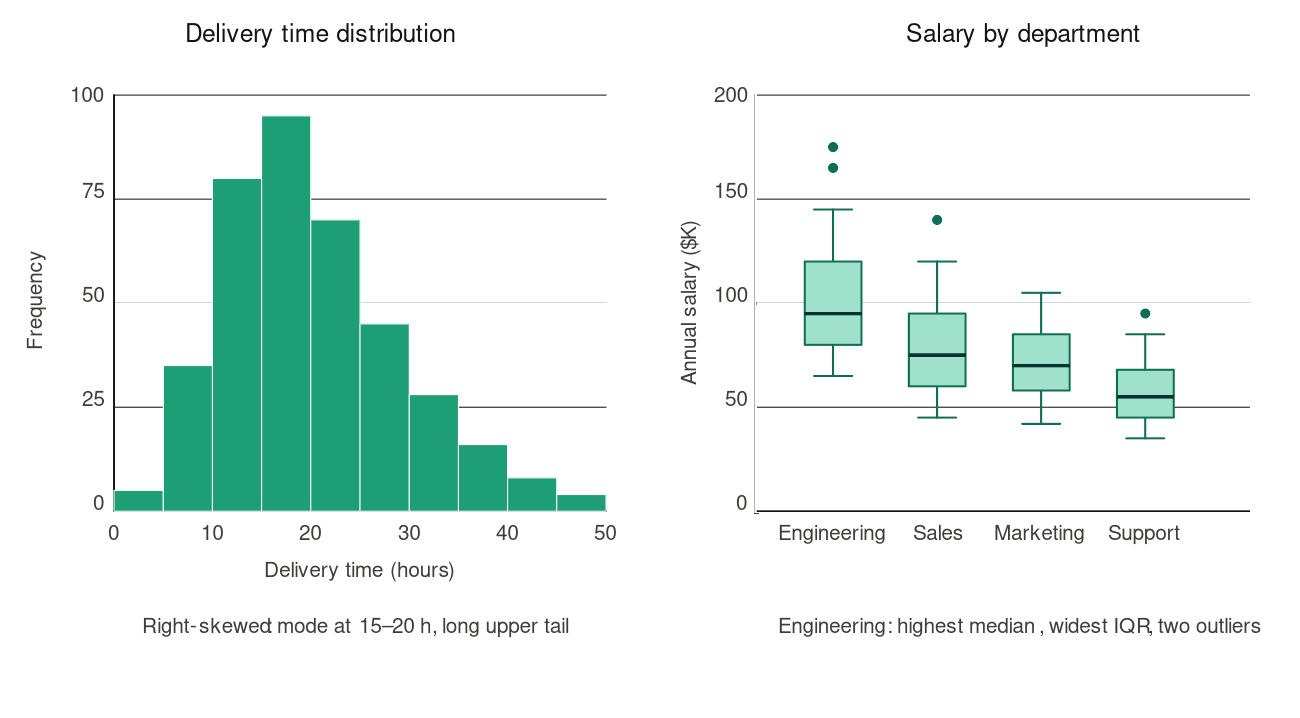
\includegraphics[width=0.85\linewidth]{slike/02/02-17.png}
    \caption{Хистограм времена испоруке и кутијасти дијаграм расподела плата по одељењима}
    \label{fig:02-7}
\end{figure}

Хистограм лево групише времена испоруке у интервале од 5 сати од 0 до 50 сати и приказује класичан десно искошен облик — већина испорука групише се око мода од 15–20 сати, са дугим репом спорих испорука које би менаџер логистике желео да испита. Кутијасти дијаграм десно сумира расподеле плата у четири одељења: свака кутија обухвата Q1 до Q3, тамна линија означава медијану, бркови се пружају до минимума и максимума унутар опсега, а тачке означавају издвојене вредности. Одељење Engineering има највишу медијану (\textasciitilde{}\$95K), најшири интерквартилни распон и две високе издвојене вредности, док је Support најниже и најуже — управо она врста међукатегоријалног поређења коју би било тешко читати из четири одвојена хистограма.

\subsubsection{Матрични подаци и топлотне мапе}
Одређени скупови података природно формирају матричну структуру, где су вредности индексиране двема категоричким или ординалним димензијама. У таквим случајевима, топлотне мапе пружају компактну и ефективну визуелизацију кодирајући вредности интензитетом боје. Конструкција укључује две дискретне променљиве пресликане на положај и једну квантитативну променљиву пресликану на боју.

Типичан пример је анализа саобраћаја на веб-сајту по сату у дану и дану у недељи. Топлотна мапа (енг. \textbf{\textit{Heatmap}}) може одмах открити периоде вршног коришћења кроз тамније области боје. Њена главна предност је у томе што брзо открива образац. Њено ограничење је што боја није добар начин за прецизно читање бројева. Зато је топлотна мапа одлична када желимо да уочимо где је нешто израженије, а мање погодна када желимо да тачно упоредимо мале разлике између вредности.

\begin{figure}[h]
    \centering
    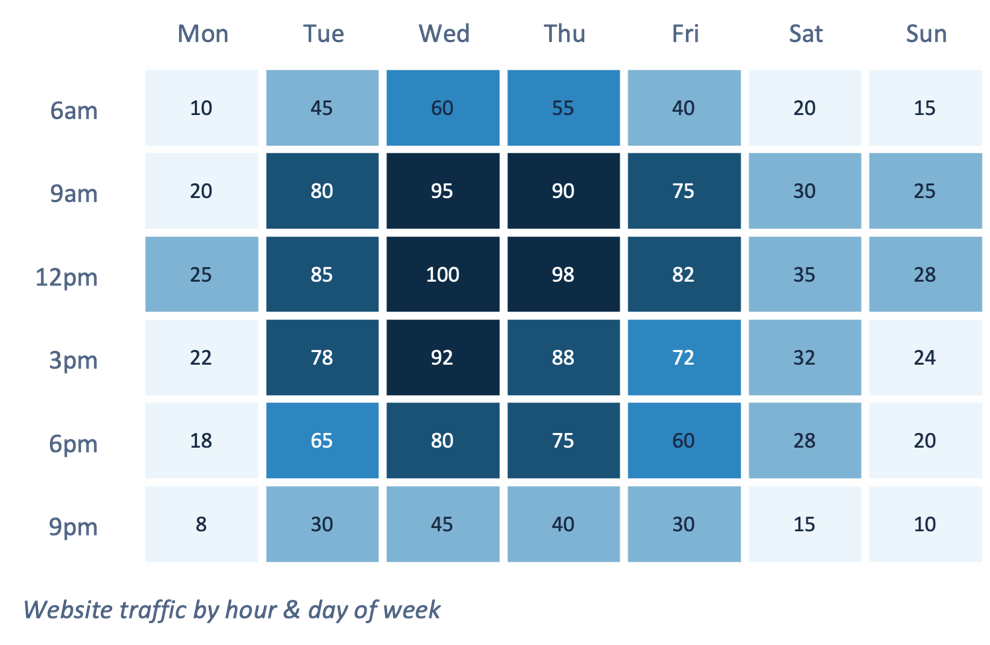
\includegraphics[width=0.85\linewidth]{slike/02/02-30.png}
    \caption{Топлотна мапа саобраћаја на веб-сајту по сату у дану и дану у недељи, која кроз интензитет боје открива периоде вршног коришћења}
    \label{fig:02-8}
\end{figure}

Топлотна мапа наслеђује и предности и ограничења утврђена у ранијим одељцима. Попут стубичастих и линијских графикона из §2.1.4, кодирање је принципијелно, а не декоративно — боја носи квантитативно значење, и сваки поступак који искривљује опажену боју искривљује и поређење. Али тамо где кодирања заснована на дужини припадају перцептивно најпоузданијем врху хијерархије графичке перцепције (Cleveland \& McGill, 1984) (§2.1.5), засићеност боје налази се знатно ниже на тој лествици: посматрачи могу рангирати интензитете боје, али из њих не могу очитати прецизне вредности. Топлотна мапа је, дакле, алат за откривање образаца — кластера, периодичности, асиметрије по матрици — а не за подршку фином квантитативном поређењу. Дизајнерска правила која следе практичне су последице овог перцептивног ограничења: избори који чувају рангирање вредности, а да притом не подстичу читаоца да доноси прецизне квантитативне судове које само кодирање не може поуздано да подржи.

Правила дизајна топлотне мапе:

\begin{itemize}
  \item Користите перцептивно уједначене скале боја (нпр. viridis)
  \item Избегавајте rainbow колор-мапе — искривљују величину
  \item \textbf{\textit{Нормализујте вредности пре поређења}}
\end{itemize}

\subsubsection{Просторни контекст и географске карте}
Када су подаци географски, просторне визуелизације као што су карте постају незаменљиве. Карте кодирају просторне променљиве кроз положај и често представљају квантитативне атрибуте помоћу боје или величине. Аналитичар јавног здравља који мапира стопе инфекције по регионима може брзо идентификовати просторне неједнакости употребом хороплет карте (енг. \textbf{\textit{choropleth map}}), под условом да су вредности адекватно нормализоване.

\begin{figure}[h]
    \centering
    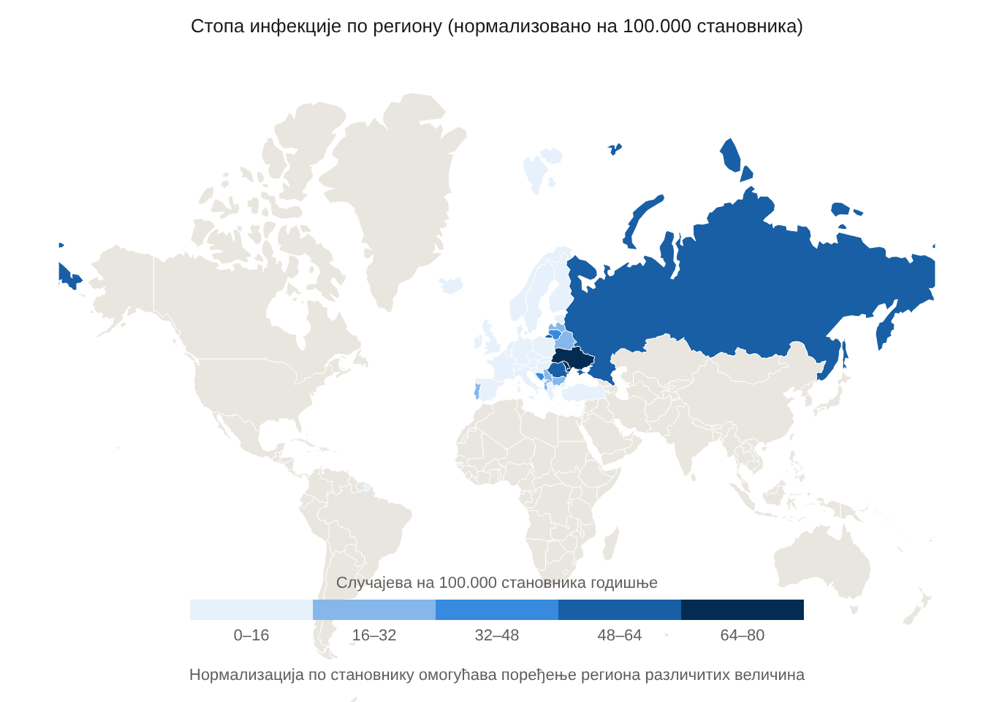
\includegraphics[width=0.85\linewidth]{slike/02/02-18.png}
    \caption{Хороплет карта стопе инфекције по регионима (случајеви на 100.000 становника), где нијанса боје кодира интензитет појаве и омогућава просторно поређење региона}
    \label{fig:02-9}
\end{figure}

Карте треба користити само када су просторни односи аналитички значајни. Коришћење карте за приказ непросторних поређења уводи непотребну сложеност и носи ризик од обмањујућег тумачења (Slocum et al., 2009).

Другим речима, карта има смисла онда када је питање по природи географско: где је проблем концентрисан, да ли постоји просторни кластер, да ли се појава шири дуж коридора, границе или урбане осе. Ако менаџера интересује само поређење укупне продаје по регионима, а географски положај региона није важан за тумачење, стубичасти графикон је обично бољи избор, јер омогућава прецизније поређење дужина него што карта омогућава поређење нијанси и површина. Карта је супериорна тек онда када позиција сама носи део значења.

Нормализација је кључна код хороплет карата. Ако се региони обоје по апсолутном броју становника, случајева болести или продаја, већи и насељенији региони ће скоро увек изгледати „важније”, чак и када је њихова стопа по становнику умерена. Зато се често приказују стопе по 1.000 или 100.000 становника, приход по купцу или број инцидената по квадратном километру. Таква нормализација омогућава фер поређење јединица различите величине. Без ње карта меша два различита питања: колико нечега има укупно и колико је појава интензивна у односу на величину популације или подручја.

Проблем постаје још израженији зато што површина региона визуелно може да завара. Велики, ретко насељени региони заузимају много простора на карти и природно привлаче пажњу посматрача, док мали, густо насељени урбани региони могу остати у другом плану иако су аналитички значајнији. Зато је добра пракса да карта буде допуњена стубичастим графиконом или табелом ранга: карта даје просторни контекст, а графикон омогућава прецизно поређење.

\subsubsection{Визуелизација неизвесности и варијабилности}
У многим аналитичким контекстима, централна тенденција података је мање информативна од њихове варијабилности и неизвесности. Игнорисање неизвесности може довести до претерано самоуверених закључака и погрешног доношења одлука, нарочито у областима као што су прогнозирање, процена ризика и анализа политика.

Неизвесност може настати услед варијабилности узорковања, грешке мерења или претпоставки модела. Визуелизација игра кључну улогу у транспарентном саопштавању ових аспеката. Традиционалне тачкасте процене, када се приказују без контекста, имплицирају лажан осећај прецизности.

На пример, ако је потребно приказати прогнозу потражње за наредни квартал, једна линија није довољна. Корисно је показати и распон у коме се стварни исход може кретати, јер тако читалац не види само очекивани тренд, већ и колико је прогноза сигурна.

Овде је важно јасно раздвојити варијабилност података од неизвесности процене. Варијабилност података означава да се сама појава природно мења од случаја до случаја: потрошња купаца, време испоруке или температура заиста варирају и када не постоји никаква грешка мерења. Неизвесност процене означава нешто друго: колико смо сигурни у неку сумарну величину или параметар који процењујемо на основу ограниченог броја опажања, на пример у просечну потражњу или у нагиб тренда. То су, дакле, два различита извора „распршености” и не смеју се тумачити као исто.

\textbf{\textit{Пример}}. Ако се посматра потрошња 100 домаћинстава, распон њихових појединачних вредности показује колико се домаћинства заиста разликују. Ако се израчуна просек и око њега се прикаже интервал поверења, тај интервал говори колико је процена просека сигурна. Ако се прикаже предиктивни интервал, онда је потребно показати у ком распону може пасти неко будуће појединачно опажање. Зато визуелизација неизвесности мора јасно да каже шта тачно приказује: варијабилност самих података, неизвесност процене или неизвесност прогнозе.

\begin{figure}[h]
    \centering
    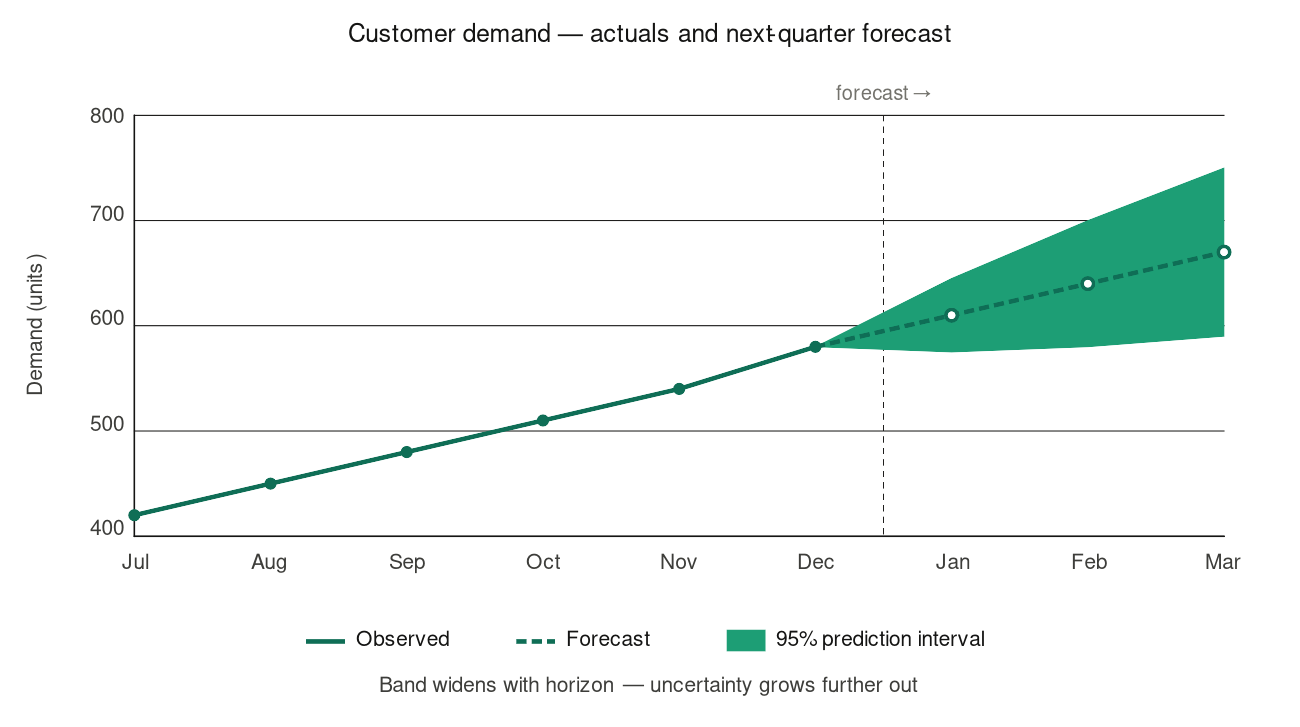
\includegraphics[width=0.85\linewidth]{slike/02/02-22.png}
    \caption{Линијски графикон са појасевима неизвесности око прогнозног тренда}
    \label{fig:02-10}
\end{figure}

Графикон приказује шест месеци посматране потражње купаца као пуну линију која расте од 420 до 580 јединица, а затим на испрекиданом вертикалном маркеру прелази у тромесечну прогнозу (610, 640, 670 јединица) исцртану испрекиданом линијом са шупљим маркерима. Засенчени тиркизни појас око прогнозе представља 95\% предиктивни интервал — узак на месту прелаза са посматраних података и све шири са хоризонтом, тако да посматрач не види само очекивану путању већ и колико је та путања поуздана у свакој тачки.

Кутијасти дијаграми нуде још један ефективан механизам за представљање варијабилности, нарочито при поређењу расподела међу групама. Када се пореде времена испоруке по логистичким провајдерима, кутијасти дијаграм открива не само просечне перформансе већ и доследност и издвојене вредности — факторе који су често релевантнији за оперативне одлуке.

\begin{figure}[h]
    \centering
    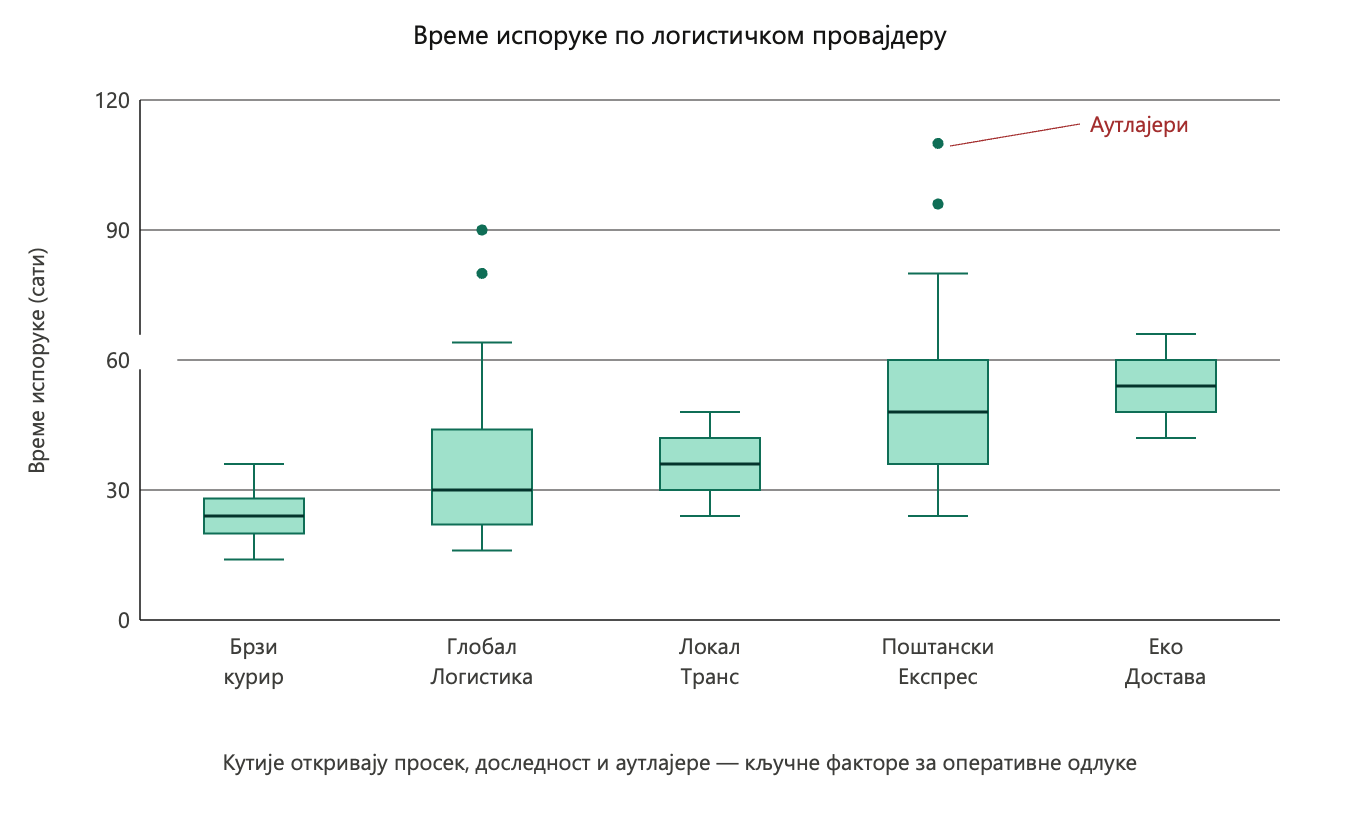
\includegraphics[width=0.85\linewidth]{slike/02/02-20.png}
    \caption{Кутијасти дијаграм времена испоруке по логистичким провајдерима — медијана, интерквартилни распон и издвојене вредности омогућавају истовремено поређење просечних перформанси, доследности и екстремних случајева међу групама}
    \label{fig:02-11}
\end{figure}

Уобичајене грешке у визуелизацији неизвесности укључују коришћење линија грешке (енг. \textbf{\textit{error bar}}) без објашњења, примену симетричних интервала на искошене расподеле или потпуно изостављање неизвесности. Такве праксе крше принцип да визуелизација треба да подржи поштену инференцију, а не само уверљиву презентацију (Tufte, 2001).

\subsection{Визуелно кодирање}
Еволуција праксе визуелизације снажно је обликована теоријским истраживањима о томе како људи опажају и тумаче визуелне информације. Кључан допринос у овој области дали су (Cleveland \& McGill, 1984), који су обезбедили емпиријску основу за графичку перцепцију. Њихов експериментални рад показао је да се различита визуелна кодирања значајно разликују по тачности када се користе за квантитативне процене (Cleveland \& McGill, 1984).

\begin{figure}[h]
    \centering
    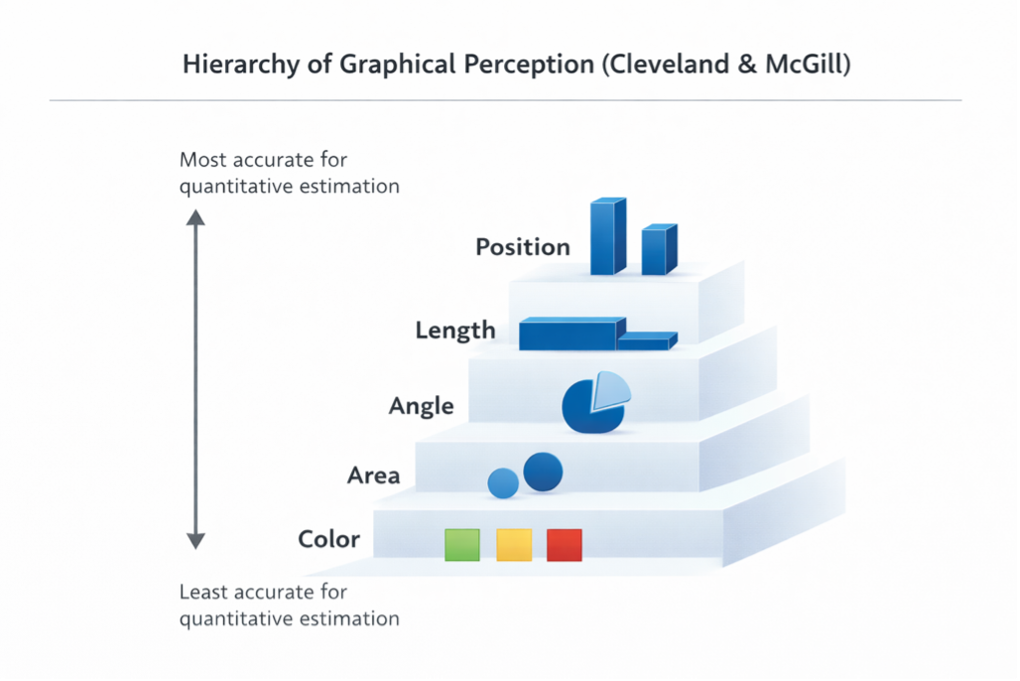
\includegraphics[width=0.85\linewidth]{slike/02/02-24.png}
    \caption{Хијерархија графичке перцепције (Cleveland \& McGill, 1984)}
    \label{fig:02-12}
\end{figure}

Истраживања показују да су прикази засновани на положају дуж исте скале тачнији за читање од приказа заснованих на дужини, углу, површини или боји. Зато су, на пример, дијаграми расејања и стубичасти графикони по правилу погоднији од кружних графикона када желимо прецизно поређење вредности.

Едвард Туфте је овај поглед допунио једноставним правилом: графикон треба да носи што више информације, а што мање сувишне декорације. Његов познати концепт односа мастила и података (енг. \textbf{\textit{data-ink ratio}}) управо то наглашава: треба смањити елементе који лепо изгледају, али не помажу разумевању (Tufte, 2001).

\begin{figure}[h]
    \centering
    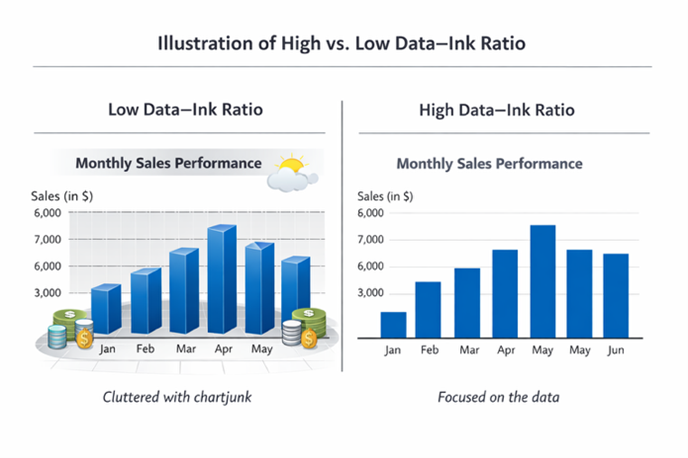
\includegraphics[width=0.85\linewidth]{slike/02/02-27.png}
    \caption{Поређење високог и ниског data–ink односа у дизајну графикона}
    \label{fig:02-13}
\end{figure}

Практичари додатно упозоравају на проблем визуелног нереда. Када графикон има превише боја, сувишних облика, анотација и декоративних линија, корисник теже уочава оно што је заиста важно. Пажња се распршује, читање постаје напорно, а образац који је потребно приказати остаје у другом плану. Зато добра визуелизација јасно истиче најважније елементе и не затрпава приказ непотребним детаљима (Few, 2012).

Ова три принципа се лако виде у пракси. Ако менаџер пореди квартални приход по пословним јединицама, стубичасти графикон ће му омогућити да разлике одмах уочи. Ако исте податке прикажемо кружним графиконом, корисник мора да процењује углове, што је мање поуздано. Ако томе додамо 3D ефекте, сенке и непотребну легенду, читање постаје још теже. У таквим случајевима графикон изгледа сложеније, а говори мање (Tufte, 2001). Зато једноставан, јасно организован графикон најчешће пружа најбољи увид.

\subsection{Вишедимензионални прикази}
Проблеми из стварног света ретко се своде на једну променљиву. Најчешће је потребно посматрати више атрибута истовремено: време, регион, производ, категорију купца, цену, количину и слично. Зато је задатак визуелизације вишедимензионалних података да помогне кориснику да у таквој сложености ипак уочи поређења, трендове и важне обрасце.

За разлику од једноставнијих приказа, овде циљ није да све променљиве „стану” у један графикон. Много је важније да се подаци паметно поделе на више повезаних приказа који омогућавају јасно поређење и постепено разумевање (Cleveland, 1993; Few, 2012).

\subsubsection{Мали вишеструки прикази}
\textbf{\textit{Мали вишеструки прикази}} (енг. \textit{small multiples}) су једна од најпрактичнијих техника за рад са вишедимензионалним подацима. Уместо једног претрпаног графикона, прави се низ сличних графикона, при чему сваки приказује један подскуп података, али са истим скалама и истим начином приказивања (Tufte, 1990).

Суштина је једноставна: ако су сви панели нацртани на исти начин, корисник ће разлике које види тумачити као разлике у подацима, а не као разлике у дизајну. Тако се поређење убрзава и читање постаје лакше.

Размотримо приход од продаје мерен током времена за више географских региона. Уместо да се сви региони прикажу у једном вишелинијском графикону — где се линије могу преклапати и постати тешко разлучиве — сваки регион може бити приказан у засебном линијском графикону распоређеном у мрежу. Време је представљено на x-оси, а приход на y-оси у сваком панелу.

\begin{figure}[h]
    \centering
    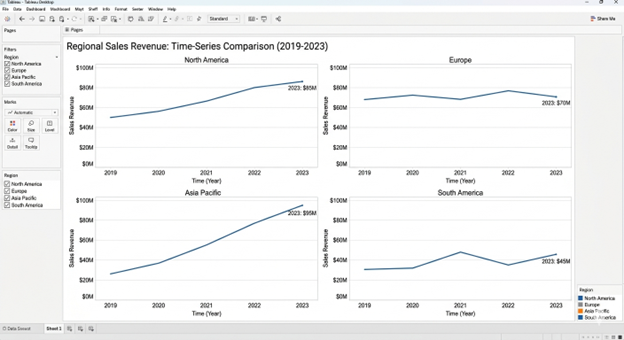
\includegraphics[width=0.85\linewidth]{slike/02/02-23.png}
    \caption{Мали вишеструки прикази (енг. small multiples) временских линијских графикона који приказују приход од продаје по регионима, уз доследне осе и скале}
    \label{fig:02-14}
\end{figure}

Ова техника најчешће укључује:

\begin{itemize}
  \item једну континуалну или временску променљиву (x-оса),
  \item \textbf{\textit{једну квантитативну меру (y-оса),}}
  \item једну категоријалну димензију која се користи за поделу података.
\end{itemize}
Мали вишеструки прикази су посебно корисни када желимо да видимо трендове, сезонске обрасце и одступања по категоријама, а да при томе не дође до преклапања елемената у једном графикону (енг. \textbf{\textit{overplotting}}). Зато се користе и када истражујемо податке и када желимо да резултат јасно објаснимо другима (Tufte, 1990; Wilke, 2019).

\subsubsection{Решеткасти прикази података}
\textbf{\textit{Фацетирање}} (енг. \textit{faceting}), односно решеткасти прикази (енг. \textit{trellis plots, lattice graphics}), проширује идеју малих вишеструких приказа тако што податке дели по једној или више категоричких димензија. Свака комбинација вредности добија свој панел, а у сваком панелу остаје исти тип графикона.

Ову технику је у статистичкој графици формализовао Cleveland (1993), а нарочито је корисна када је потребно видети како се односи у подацима мењају кроз више категорија.

Претпоставимо да се резултати задовољства купаца анализирају по категоријама производа и сегментима купаца током времена. Фацетирани распоред може поставити категорије производа у редове, а сегменте купаца у колоне, при чему сваки панел приказује временску серију оцена задовољства.

\begin{figure}[h]
    \centering
    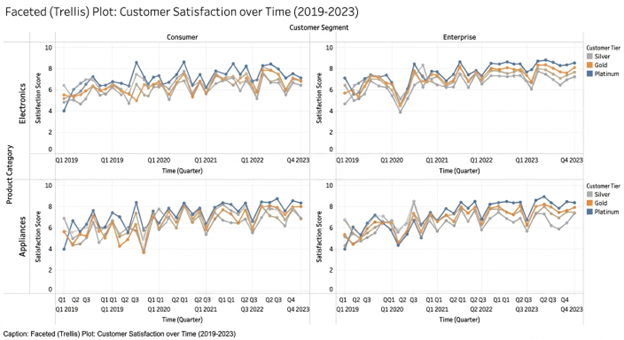
\includegraphics[width=0.85\linewidth]{slike/02/02-31.png}
    \caption{Фацетирани (енг. trellis) графикон задовољства купаца током времена, распоређен по категорији производа (редови) и сегменту купаца (колоне)}
    \label{fig:02-15}
\end{figure}

Фацетирање најчешће укључује:

\begin{itemize}
  \item једну или две категоријалне променљиве које се користе за распоред панела,
  \item једну или више квантитативних променљивих приказаних унутар панела,
  \item фиксно графичко кодирање које се понавља кроз све панеле.
\end{itemize}
Савремени алати као што су Tableau и ggplot2 третирају фацетирање као основну технику, јер омогућава да се сложени подаци прикажу прегледно и без губитка јасноће (Few, 2012; Munzner, 2014).

\subsubsection{Изазови визуелизације високодимензионалних података}
Ипак, ни мали вишеструки прикази ни фацетирање не решавају све проблеме. Када број димензија превише порасте, расте и ризик да приказ постане претрпан или да корисник погрешно протумачи оно што види.

Основно ограничење је у томе што људи могу поуздано да прочитају само ограничен број визуелних канала, а положај и дужина су и даље много прецизнији од боје или облика (Cleveland \& McGill, 1984).

Изазови визуелизације високодимензионалних података најчешће укључују:

\begin{itemize}
  \item \textbf{\textit{преклапање исцртаних елемената}} (енг. \textit{overplotting}),
  \item смањену интерпретабилност сложених кодирања,
  \item тешкоћу очувања смислених односа растојања.
\end{itemize}
Зато се у пракси често користе:

\begin{itemize}
  \item технике смањења димензионалности (нпр. Анализа главних компонената) пре визуелизације,
  \item интерактивне механизме као што су филтрирање, означавање избора (енг. \textit{brushing}) и увећавање приказа (енг. \textit{zooming}),
  \item повезане приказе, где више координисаних графикона заједно представља различите пројекције истих података.
\end{itemize}
У контролним таблама овакви подаци најбоље функционишу када се сложеност открива постепено, кроз интеракцију. Корисник прво види општу слику, а затим по потреби улази дубље. Зато су интеракција и координисани прикази важан део савремене визуелне аналитике (Few, 2013; Munzner, 2014). Технике интеракције и израде контролних табли биће описане у §§2.1.8 и 2.1.9 и Одељку 6.

\subsection{Приповедање}
\textbf{\textit{Приповедање помоћу података}} (енг. \textit{storytelling with data}) подразумева представљање резултата анализе података тако да публика разуме шта је важно и зашто је то важно. За разлику од експлораторне визуелизације, где корисник слободно истражује податке, овде је нагласак на јасној комуникацији и вођењу публике ка одређеном увиду, тумачењу или препоруци (Segel \& Heer, 2010; Knaflic, 2015).

Основа доброг приповедања помоћу података је јасна наративна структура. Она публици помаже да прати ток приче, разуме податке и запамти главни закључак. У пракси, већина оваквих прича прати једноставан редослед: контекст, развој проблема, кључни увид и последица или препорука (Kosara \& Mackinlay, 2013).

Често прихваћен оквир укључује следеће компоненте:

\begin{itemize}
  \item \textbf{\textit{Контекст и мотивација}}: Увођење домена проблема, аналитичког питања и релевантности података.
  \item \textbf{\textit{Аналитичка тензија}}: Представљање кључних поређења, трендова или аномалија који отварају питања или откривају неизвесност.
  \item \textbf{\textit{Разрешење и увид}}: Истицање централних аналитичких налаза изведених из података.
  \item \textbf{\textit{Импликације и акција}}: Повезивање увида са одлукама, препорукама или стратешким поступцима.
\end{itemize}
Суштина је да визуелизација не треба само да покаже податке, већ и да помогне публици да дође до исправног закључка (Tufte, 2001). У пословној интелигенцији и контролним таблама (које ће бити објашњене у каснијем тексту) то се често постиже пажљивим редоследом приказа, постепеним откривањем детаља и јасним повезивањем са кључним показатељима перформанси (енг. \textbf{\textit{key performance indicators}}, KPI) (Few, 2013). Важно је напоменути да приповедање на основу података није обавезно везано за контролне табле већ и за појединачне визуелизације. 

Основне технике које се користе у приповедању на основу података су: \textbf{\textit{анотација}} и \textbf{\textit{контекстуализација}}. Анотација и контекстуализација помажу да се значење угради директно у графикон. И када је приказ добро дизајниран, кратак текстуални сигнал често помаже кориснику да одмах разуме шта треба да примети и зашто је то важно (Knaflic, 2015).

Анотације могу укључивати:

\begin{itemize}
  \item Дескриптивне ознаке које идентификују критичне вредности или догађаје.
  \item Објашњавајуће напомене које разјашњавају трендове, аномалије или прекиде у обрасцима.
  \item Контекстуалне маркере који повезују тачке података са спољним догађајима, променама политика или пословним одлукама.
\end{itemize}

\begin{figure}[h]
    \centering
    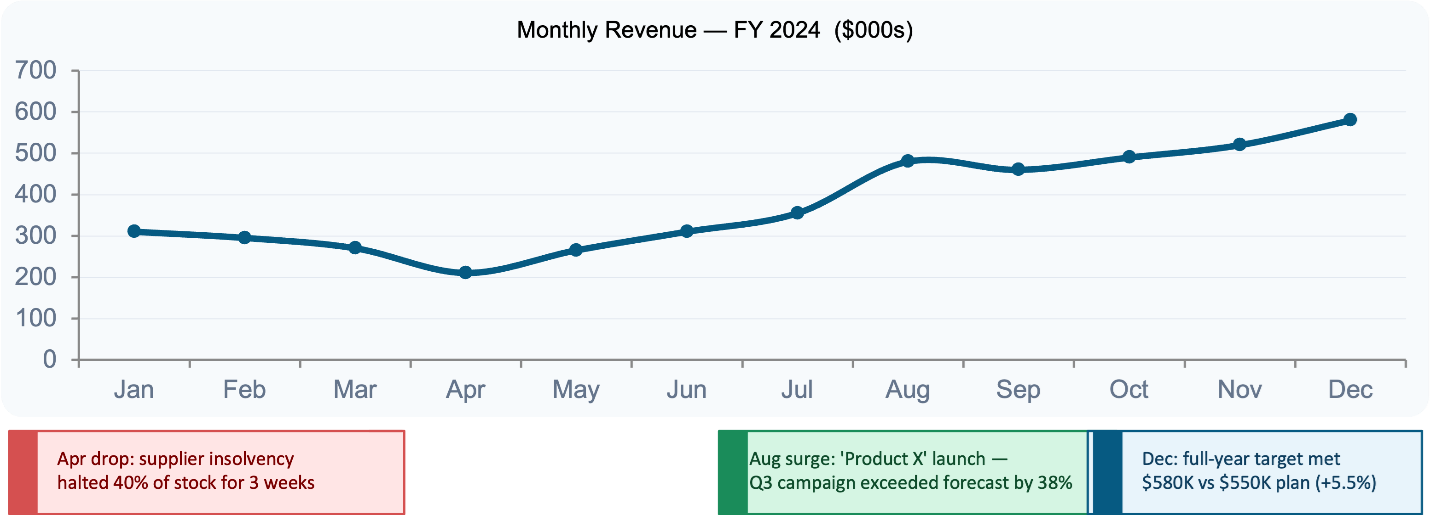
\includegraphics[width=0.85\linewidth]{slike/02/02-21.png}
    \caption{Анотирани графикон који повезује уочене обрасце са пословним догађајима}
    \label{fig:02-16}
\end{figure}

На слици су анотацијама истакнути кључни тренутни догађаји који објашњавају скокове и падове у временској серији. Текстуалне ознаке су повезане са одговарајућим тачкама на графикону, чиме је читаоцу омогућено да уочене обрасце директно повеже са пословним контекстом, без посебне референце на додатну табелу или текст.

Истраживања графичке перцепције показују да људи не изводе сами увек исти закључак само на основу обрасца који виде (Cleveland \& McGill, 1984). Зато анотације имају важну улогу: оне усмеравају пажњу и помажу да се визуелни образац повеже са правилним тумачењем. То је посебно важно када се на основу графикона доносе озбиљне пословне одлуке.

\subsection{Интеракција над визуелизацијама}
Технике интеракције су кључни део савремених система за визуелизацију и визуелну аналитику. За разлику од статичких приказа, интерактивна визуелизација омогућава кориснику да мења поглед на податке, пореди различите перспективе и постепено проверава своје претпоставке. Тако визуелизација постаје радни простор за размишљање, а не само средство приказивања резултата (Card, Mackinlay, \& Shneiderman, 1999; Keim et al., 2008).

Интеракција у пракси помаже кориснику да мање памти, а више проверава хипотезе директно на приказу (Ware, 2013). У алатима као што су \textit{Tableau}, \textit{Power BI} и веб-засноване контролне табле, филтрирање, означавање избора (енг. \textit{brushing}), увећавање приказа (енг. \textit{zooming}), продубљивање увида (енг. \textit{drill-down}), истицање и динамичка агрегација помажу да се сложени подаци читају корак по корак.

\subsubsection{Филтрирање}
\textbf{\textit{Филтрирање}} (енг. \textit{filtering}) значи да се на приказу задржи само онај део података који је тренутно важан. Тако се смањује визуелни неред и пажња усмерава на релевантан подскуп. Филтери могу бити категоријални, на пример избор региона или групе производа, или нумерички, као што је ограничење на одређени опсег вредности.

У експлораторној анализи филтрирање омогућава брзо поређење различитих подскупова података и тако подстиче стварање и проверу хипотеза (Tukey, 1977). На пример, аналитичар може филтрирати продају по периоду, сегменту купаца или региону да би видео да ли се проблем јавља свуда или само у појединим деловима пословања. На контролним таблама филтери су најчешће реализовани као падајући менији, клизачи или поља за избор.

Посматрано из угла корисничког искуства, филтрирање прати принцип фокус уз контекст (енг. \textbf{\textit{focus plus context}}): корисник се усмерава на важан део података, али и даље задржава свест о широј слици (Shneiderman, 1996).

\subsubsection{Означавање и повезивање}
\textbf{\textit{Означавање избора}} (енг. \textit{brushing}) значи да корисник интерактивно означи неки део приказа, на пример групу тачака или један опсег стубаца, а систем их визуелно истакне. Када је то повезано са више приказа (енг. \textit{linking}), исти избор се одмах види и у другим графиконима.

Ова техника је посебно корисна у мултиваријантној анализи, где један графикон често није довољан. На пример, ако се у раштрканом дијаграму означи група издвојених вредности, може се одмах видети како се ти исти елементи понашају у паралелним координатама (енг. \textit{parallel coordinates}), кутијастом дијаграму (енг. \textit{box plot}) или на карти (Becker \& Cleveland, 1987).

Означавање и повезивање приказа помажу кориснику да провери да ли се исти образац појављује у више различитих графикона (Heer \& Shneiderman, 2012). Зато су они основа система координисаних вишеструких приказа (енг. \textit{coordinated multiple views}, CMV).

\subsubsection{Увећавање и померање}
\textbf{\textit{Увећавање приказа}} (енг. \textit{zooming}) омогућава кориснику да пређе са опште слике на детаље, док померање приказа (енг. \textit{panning}) омогућава кретање кроз различите делове простора приказа. Ове технике су посебно важне код великих скупова података, карата и временских серија.

У временској анализи ово омогућава прелаз са дугорочних трендова на краткорочне промене, па корисник лакше уочава сезонске ефекте, прекиде у кретању или локалне аномалије. Код карата су увећавање и померање основни облици интеракције.

Shneiderman-ова мантра тражења информација — „прво преглед, затим увећање и филтрирање, па тек онда детаљи на захтев” (енг. overview first, zoom and filter, then details on demand) — истиче увећавање приказа као кључни корак у аналитичком току рада (Shneiderman, 1996).

\subsubsection{Продубљивање и агрегирање}
\textbf{\textit{Продубљивање увида}} (енг. \textit{drill-down}) значи да корисник са општег нивоа може да пређе на све детаљније нивое података, на пример са године на квартал, па на месец. Супротно томе, сажимање на виши ниво (енг. \textit{roll-up}) враћа приказ на општији ниво.

Ове технике су повезане са \textbf{\textit{OLAP}}-ом, односно аналитичком обрадом на мрежи (енг. \textit{online analytical processing}), и веома су честе у ПИ контролним таблама (Kimball \& Ross, 2013). Ови концепти ће бити објашњени у каснијем тексту. Продубљивање и агрегирање омогућавају да корисник прати образац са високог нивоа до његовог конкретног узрока, на пример да види који производи или региони највише доприносе паду прихода.

Да би ови механизми били корисни, хијерархије (нивои агрегирања) морају бити интуитивне и у складу са начином на који корисник размишља о домену.

\subsubsection{Технике истицања и фокусирања}
Истицање наглашава изабране елементе бојом, величином или анотацијом, док остали елементи остају у другом плану. За разлику од филтрирања, овде цео скуп података остаје видљив, па корисник не губи контекст.

Ова техника је посебно корисна у објашњавању и приповедању, када желимо да пажњу усмеримо на један важан образац, а да ипак задржимо ширу слику (Few, 2012; Segel \& Heer, 2010). На пример, могуће је истаћи једну линију тренда, а остале оставити блеђе у позадини.

Истицање је важно и за анализу, јер помаже корисницима да брже уоче важне елементе у сложеним приказима.

\subsubsection{Динамичка агрегација}
Динамичка агрегација омогућава кориснику да интерактивно мења ниво сажимања података, тако да систем одмах поново израчуна укупне износе, просеке или расподеле на основу тренутних избора. За разлику од унапред припремљених агрегата, овде се резултат мења заједно са интеракцијом корисника.

Ово је веома важно у истраживачкој аналитици, јер корисник може да провери како се исти подаци понашају када се групишу на различите начине (Keim et al., 2008). На пример, купце је могуће груписати по региону, старосној групи или учесталости куповине и видети да ли се образац мења.

У савременим системима то се најчешће реализује кроз параметре и контроле које кориснику дозвољавају да сам бира начин груписања и функцију агрегације. Тако анализа постаје постепен и интерактиван процес.

\subsection{Пивот табеле}
\textbf{\textit{Пивот табела}} (енг. \textit{pivot table}) је алат за визуализацију података који омогућава интерактивну манипулацију података. Пивот табела се може описати као образац за креирање табеларног извештаја. Основни елементи пивот табеле су:

Подаци се групишу по једном или више атрибута у редовима и колонама, док се квантитативне вредности агрегирају збиром, средњом вредношћу, бројем, минимумом, максимумом или другим функцијама. Преуређивањем атрибута се добијају нови погледи без поновног упита над изворним подацима.

Концептуално, пивот табела имплементира операције: ротирање димензија (енг. \textit{pivot}), сужавање нивоа агрегације (енг. \textit{roll-up}) и његово продубљивање (енг. \textit{drill-down}), као и фокусирање на подскуп података (енг. \textit{slice and dice}). За разлику од класичних извештаја, којима је структура унапред фиксирана, пивот табела се користи као алат за истраживачку анализу јер кориснику дозвољава да аналитичка питања постави и преформулише у току рада (Few, 2013; Sharda et al., 2020).

Типичан пример је анализа продаје: трансакциони запис се своди на квантитативну меру (приход) и неколико категоричких димензија (регион, категорија производа, канал продаје, месец). Постављањем региона у редове и категорије у колоне се добија матрица прихода која се у наредном кораку реструктурира — нпр. заменом региона каналом продаје или прелазом са месечне на кварталну агрегацију — без писања новог упита и без напуштања приказа.

Ефективност пивот табеле зависи од квалитета изворних података и од начина на који су димензије моделиране. Препоручује се да изворни подаци буду у дугачком (нормализованом) формату, где је сваки ред једно опажање, а сваки атрибут засебна колона (Wickham, 2014). Хијерархије димензија (нпр. држава → регион → град или година → квартал → месец) треба да буду конзистентно дефинисане, јер се на њима ослањају операције roll-up и drill-down. Када су димензије хетерогене или непотпуне, агрегати постају нетачни, а поређења између група обмањујућа.

Савремене ПИ платформе (\textit{Excel}, \textit{Power BI}, \textit{Tableau}, \textit{Looker}) и програмски алати (\textit{pandas}, \textit{dplyr}) подржавају пивот функционалност као основни механизам сажимања података. У контексту контролних табли, пивот табела се често користи као сирови приказ испод визуелизације — корисник прелази са графикона на нумеричке вредности ради верификације и даљег испитивања (Knaflic, 2020). У ширем оквиру подршке одлучивању, пивот табеле представљају мост између дескриптивне аналитике и интерактивне визуелне аналитике, јер исту операцију агрегације чине доступном и техничким и не-техничким корисницима.

\subsection{Контролне табле}
Контролна табла је визуелни интерфејс који на једном месту окупља кључне информације потребне за праћење рада, анализу и доношење одлука. Основна сврха контролне табле је да помогне кориснику да од података дође до увида који води ка конкретној акцији. Контролне табле је могуће дефинисати и као скуп визуализација које могу бити контролисане применом техника интеракције. За разлику од општих приказа података, добра контролна табла треба да омогући кориснику да на први поглед разуме тренутно стање, уочи проблем и види где треба да усмери пажњу (Few, 2013; Eckerson, 2010).

У ширем оквиру система за подршку одлучивању (DSS), контролне табле су интерфејси који повезују инфраструктуру података са људским расуђивањем. Оне не замењују знање корисника нити саму анализу, већ помажу да важне информације буду брже видљиве и смислено организоване (Shneiderman, 1996; Ware, 2013).

Зато се контролне табле не оцењују само по томе да ли лепо изгледају или да ли технички раде брзо, већ и по томе да ли заиста помажу кориснику да постави приоритете и предузме праву акцију у стварном организационом окружењу.

Из угла визуелне аналитике, контролна табла помаже да сложени односи у подацима постану прегледни и лакши за тумачење. Њена вредност не зависи само од тога да ли су подаци тачни, већ и од тога да ли су добро организовани, јасно приказани и прилагођени задатку корисника (Ware, 2013).

Већина савремених дефиниција наглашава неколико основних карактеристика контролних табли:

\begin{itemize}
  \item Интеграцију више индикатора унутар једног екрана или ограниченог броја приказа
  \item Употребу визуелних кодирања оптимизованих за брзу перцепцију
  \item Усклађеност са конкретним аналитичким или оперативним циљевима
  \item Подршку праћењу, истраживању или и једном и другом
\end{itemize}
У свим овим категоријама контролна табла треба да уравнотежи једноставност и дубину: да одмах да одговор на основна питања, али и да омогући кориснику да, ако је потребно, истражи детаље кроз интеракцију, филтере и продубљивање увида (енг. \textit{drill-down}) (Keim et al., 2010).

Иако се о контролним таблама и извештајима често говори заједно, они се суштински разликују по сврси, структури и начину употребе. Извештаји су обично статички или полустатички документи који доносе унапред припремљене табеле, сажетке и графиконе. Најчешће се праве периодично и намењени су ретроспективној анализи, формалној комуникацији или евиденцији (Few, 2013). Зато су усмерени више на потпуност и документацију него на брзо визуелно читање. Контролне табле су, насупрот томе, намењене континуираној употреби и наглашавају брзину читања, избор најважнијих показатеља и визуелну јасноћу. 

Кључне разлике укључују:

\begin{itemize}
  \item Временску оријентацију: контролне табле наглашавају текуће стање и трендове, док извештаји наглашавају историјске сажетке
  \item Интеракцију: контролне табле обично подржавају филтрирање, унакрсно истицање и продубљивање увида (енг. \textit{drill-down}), док су извештаји углавном статички
  \item Когнитивни циљ: контролне табле подржавају праћење и разумевање ситуације, док извештаји подржавају објашњење и вођење евиденције
\end{itemize}
Аналитичке апликације иду корак даље од контролних табли, јер визуелизацију повезују са ширим окружењем напредне аналитике, машинског учења, статистичких модела и правила специфичних за домен. Док контролна табла пре свега приказује индикаторе и сажетке, аналитичка апликација подржава сложеније задатке као што су тестирање хипотеза, анализа сценарија, предвиђање и оптимизација.

Из угла архитектуре, контролне табле су најчешће део презентационог слоја, док аналитичке апликације у истом окружењу повезују приказ, аналитичке моделе и пословна правила (Keim et al., 2010). На пример, продајна контролна табла може приказивати трендове прихода и резултате по регионима, док аналитичка апликација може омогућити симулацију цена, процену узрока и покретање предиктивних модела.

Разлика се може сажети на следећи начин:

\begin{itemize}
  \item Контролне табле одговарају на питања „Шта се дешава?” и „Где треба да погледам?”
  \item Аналитичке апликације баве се питањима „Зашто се то дешава?” и „Шта ће се догодити ако…?”
\end{itemize}
Упркос овим разликама, савремене ПИ платформе све више замагљују границу између контролних табли и аналитичких апликација уграђивањем напредне аналитике, излаза машинског учења и вођене анализе директно у интерфејсе контролних табли (Davenport \& Harris, 2007; Knaflic, 2020).

Контролне табле се најчешће деле према сврси, временском хоризонту и нивоу одлучивања који подржавају. Иако све имају заједнички циљ да помогну кориснику да брже разуме податке, њихов дизајн, ниво детаља, интеракција и захтеви у погледу перформанси разликују се у зависности од тога да ли служе оперативним, тактичким или стратешким одлукама (Few, 2013; Eckerson, 2011; Sharda et al., 2020).

\textbf{\textit{Оперативне контролне табле}} служе свакодневном праћењу процеса и брзом реаговању. Њихов циљ је да покажу шта се дешава управо сада, где постоји проблем и где је потребна непосредна интервенција. Најчешће их користе супервизори, оперативни менаџери и запослени који су блиско повезани са самим процесом.

Оне се ослањају на податке у реалном или скоро реалном времену, који се освежавају у кратким интервалима. Приказани подаци су детаљни и тесно везани за конкретне активности, као што су испоруке, доступност система, ток производње или време одзива услуге (Eckerson, 2011).

Кључне карактеристике оперативних контролних табли укључују:

\begin{itemize}
  \item Високу учесталост освежавања података (секунде до минуте)
  \item Нагласак на индикаторима статуса и упозорењима
  \item \textbf{\textit{Ограничен историјски контекст}}
  \item Снажно ослањање на унапред дефинисане прагове и правила
\end{itemize}
Уобичајени визуелни елементи укључују мераче, статусна светла, мини линијске графиконе (енг. \textbf{\textit{sparklines}}), стубичасте графиконе и табеле са условним форматирањем. Боја се често користи да скрене пажњу на изузетке, на пример кодирањем црвено-жуто-зелено, иако претерана употреба таквих шема може смањити јасноћу ако нису пажљиво дизајниране (Few, 2013).

Оперативне контролне табле су тесно усклађене са дескриптивном аналитиком, одговарајући на питања као што су „Шта се дешава управо сада?” и „Где је потребна непосредна акција?” (Sharda et al., 2020). Интеракција је типично ограничена на филтрирање или продубљивање увида (енг. \textbf{\textit{drill-down}}), јер се брзини и јасноћи даје приоритет у односу на истраживачку анализу.

\begin{figure}[h]
    \centering
    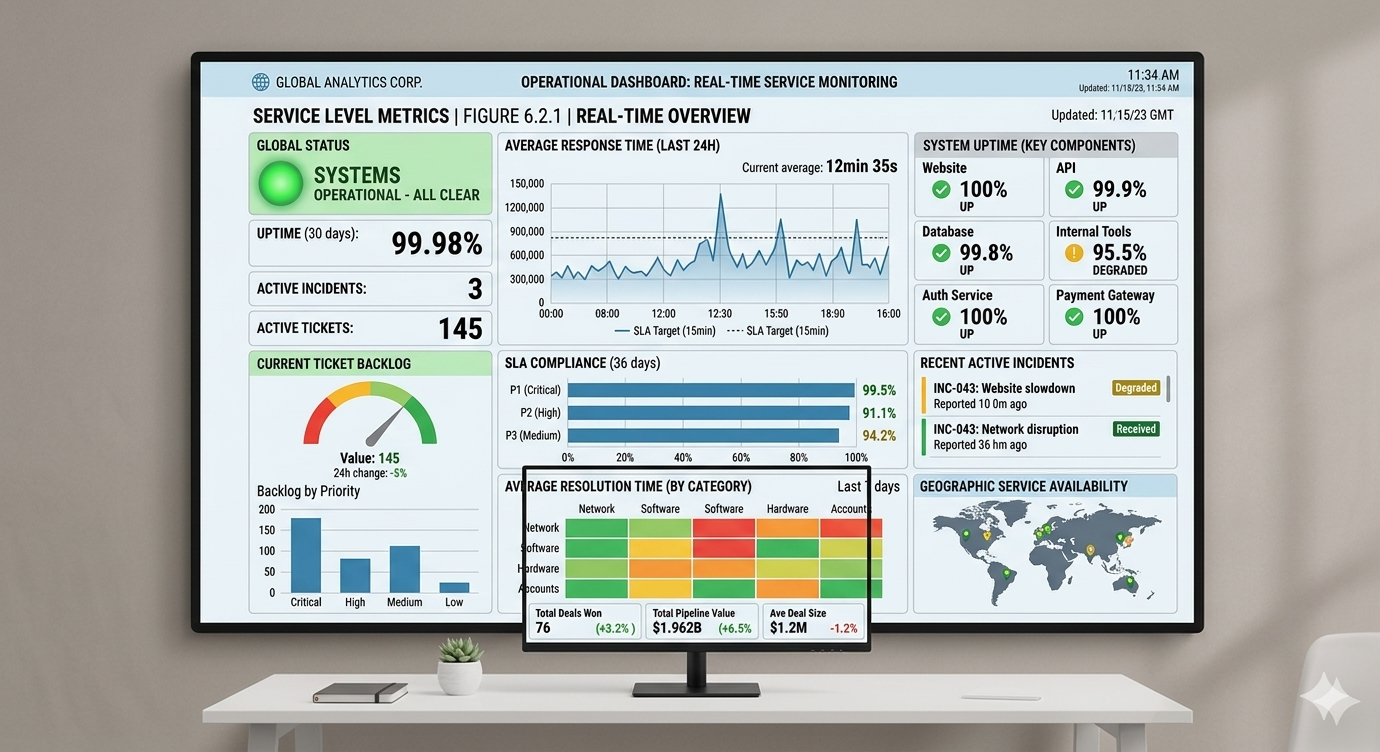
\includegraphics[width=0.85\linewidth]{slike/02/02-32.png}
    \caption{Пример оперативне контролне табле за праћење метрика нивоа услуге у реалном времену}
    \label{fig:02-17}
\end{figure}

\textbf{\textit{Тактичке контролне табле}} подржавају краткорочно и средњорочно одлучивање, типично на нивоу одељењског или функционалног менаџмента. Њихова примарна сврха је да процене трендове перформанси, упореде исходе са циљевима и ефикасније расподеле ресурсе.

За разлику од оперативних контролних табли, тактичке контролне табле ослањају се на агрегиране и сажете податке, често у распону од више недеља или месеци. Оне комбинују историјски контекст са недавним перформансама, омогућавајући корисницима да идентификују обрасце, неефикасности и настајуће ризике (Eckerson, 2011).

Кључне карактеристике тактичких контролних табли укључују:

\begin{itemize}
  \item Периодична ажурирања података (дневно, недељно)
  \item Нагласак на трендовима, поређењима и упоредним показатељима (енг. \textit{benchmark indicators})
  \item \textbf{\textit{Умерен ниво интерактивности}}
  \item Интеграцију више међусобно повезаних метрика
\end{itemize}
Типични аналитички задаци које подржавају тактичке контролне табле укључују поређење по категоријама (нпр. региони, тимови), анализу трендова током времена и анализу одступања у односу на унапред дефинисане циљеве или кључне показатеље перформанси (енг. \textbf{\textit{key performance indicators}}, KPI). Визуелизације као што су линијски графикони, груписани стубичасти графикони, топлотне мапе и мали вишеструки прикази (енг. \textbf{\textit{small multiples}}) уобичајено се користе за подршку овим задацима (Few, 2013).

\textbf{\textit{Тактичке контролне табле}} заузимају централну позицију између дескриптивне и дијагностичке аналитике, бавећи се питањима као што су „Зашто остварујемо боље или лошије резултате од очекиваних?” и „Које области захтевају корективну акцију?” (Sharda et al., 2020). Технике интеракције као што су унакрсно филтрирање и продубљивање увида (енг. \textbf{\textit{drill-down}}) посебно су важне, јер омогућавају менаџерима да пређу са сажетака високог нивоа на детаљније приказе.

\begin{figure}[h]
    \centering
    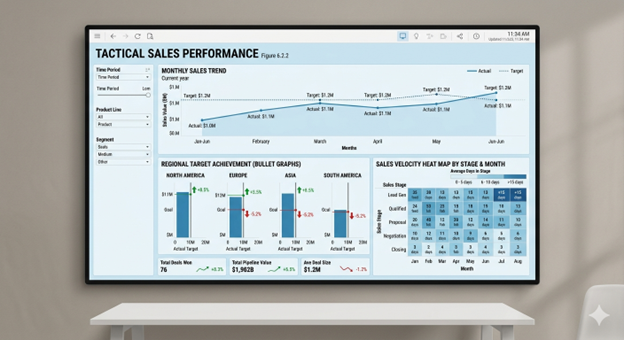
\includegraphics[width=0.85\linewidth]{slike/02/02-26.png}
    \caption{Тактичка контролна табла која приказује месечне продајне перформансе по регионима}
    \label{fig:02-18}
\end{figure}

Стратешке контролне табле намењене су подршци дугорочном одлучивању високог нивоа од стране виших руководилаца и топ менаџмента. Њихова примарна улога је да пруже интегрисан приказ организационих перформанси усклађен са стратешким циљевима.

Стратешке контролне табле типично се фокусирају на мали број критичних метрика, често изведених из оквира као што је Уравнотежени систем показатеља (енг. \textit{Balanced Scorecard}). Нагласак је на јасноћи, усклађености са циљевима и комуникацији, а не на детаљној анализи (Kaplan \& Norton, 1996; Few, 2013).

Кључне карактеристике стратешких контролних табли укључују:

\begin{itemize}
  \item Ниску учесталост освежавања података (месечно, квартално)
  \item \textbf{\textit{Висок ниво агрегације}}
  \item Снажну повезаност са стратешким циљевима и иницијативама
  \item Минималну, али пажљиво дизајнирану интерактивност
\end{itemize}
Визуелни дизајн у стратешким контролним таблама даје приоритет једноставности и доследности. Прекомерна количина детаља или сложена визуелна кодирања могу замаглити укупну поруку и смањити поверење руководилаца у контролну таблу као алат за подршку одлучивању (Few, 2013). Уобичајени визуелни облици укључују сажете KPI плочице, линије тренда и графиконе поређења високог нивоа.

\textbf{\textit{Стратешке контролне табле}} превасходно су повезане са експланаторном и прескриптивном аналитиком, бавећи се питањима као што су „Да ли смо на путу да остваримо наше стратешке циљеве?” и „Којим стратешким иницијативама треба дати приоритет?” (Sharda et al., 2020). Иако је интеракција ограничена, руководиоци могу селективно користити продубљивање увида (енг. \textbf{\textit{drill-down}}) да би проверили претпоставке или истражили узроке великих одступања.

\begin{figure}[h]
    \centering
    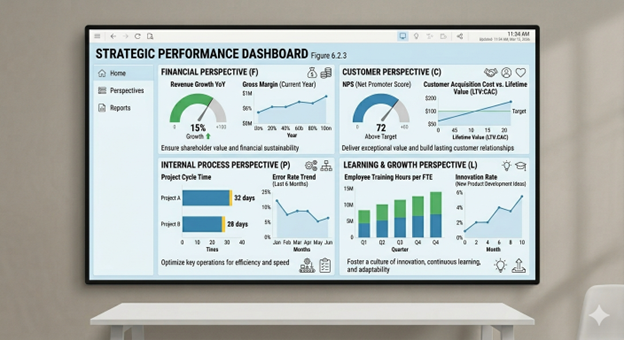
\includegraphics[width=0.85\linewidth]{slike/02/02-29.png}
    \caption{Стратешка контролна табла усклађена са оквиром Balanced Scorecard}
    \label{fig:02-19}
\end{figure}

Иако се оперативне, тактичке и стратешке контролне табле разликују по сврси и дизајну, не треба их посматрати као изоловане артефакте. У зрелим аналитичким окружењима, контролне табле на различитим нивоима логички су повезане, омогућавајући кохерентан ток од стратешких циљева ка тактичким иницијативама и оперативном извршењу (Eckerson, 2011).

\begin{table}[h]
\centering
    \caption{Поређење оперативних, тактичких и стратешких контролних табли}
    \label{tab:02-1}
\begin{adjustbox}{max width=\textwidth}
\begin{tabular}{|l|l|l|l|}
\hline
\textbf{\textit{Атрибут}} & \textbf{\textit{Оперативне}} & \textbf{\textit{Тактичке}} & \textbf{\textit{Стратешке}} \\
\hline
\textbf{\textit{Ниво одлучивања}} & Свакодневно праћење процеса; супервизори и оперативни менаџери & Краткорочно и средњорочно; одељењски/функционални менаџмент & Дугорочно; виши руководиоци и топ менаџмент \\
\hline
\textbf{\textit{Грануларност података}} & Детаљни подаци везани за конкретне активности & Агрегирани и сажети подаци (недеље/месеци) & Високо агрегиране метрике на нивоу организације \\
\hline
\textbf{\textit{Учесталост ажурирања}} & Реално или скоро реално време (секунде до минуте) & Периодично (дневно, недељно) & Ниска учесталост (месечно, квартално) \\
\hline
\textbf{\textit{Аналитички фокус}} & Дескриптивна аналитика — „Шта се дешава сада?” & Дескриптивна и дијагностичка — „Зашто резултати одступају?” & Експланаторна и прескриптивна — „Да ли смо на путу ка стратешким циљевима?” \\
\hline
\end{tabular}
\end{adjustbox}
\end{table}
Архитектура контролне табле дефинише техничку и логичку структуру која омогућава контролним таблама да поуздано трансформишу сирове податке у увиде који омогућавају деловање. Архитектура контролне табле треба се разумети не само као слој визуелизације, већ као интегрисана компонента ширег аналитичког екосистема, која обухвата изворе података, логику трансформације, семантичку апстракцију, технологије складиштења и механизме извршавања упита. Добро пројектоване архитектуре контролних табли уравнотежују перформансе, скалабилност, управљање подацима и аналитичку флексибилност, уз обезбеђивање доследности метрика и тумачења међу организационим корисницима (Chaudhuri, Dayal, \& Narasayya, 2011; Few, 2013). 

\subsection{Алати за креирање контролних табли и интерактивних извештаја}
Алати за визуелизацију и израду контролних табли се обично деле у три групе: платформе пословне интелигенције (ПИ), алате засноване на програмирању и веб-базиране оквире. Свака група има различиту намену, профил корисника и техничке могућности, па се избор доноси у односу на аналитичке захтеве, профил тима и шири аналитички екосистем.

ПИ платформе (\textit{Tableau}, \textit{Power BI}, \textit{Qlik Sense}, \textit{Looker}) покривају цео ток рада — повезивање са подацима, моделирање, израду контролних табли и дељење. Њихова основна предност је самостална аналитика: корисник без техничког предзнања истражује податке кроз „превуци и пусти” интерфејсе, док семантички слојеви и израчуната поља сакривају техничку сложеност (Few, 2013; Kimball \& Ross, 2013). Платформе су тесно повезане са складиштима података и OLAP системима, и подржавају и аналитику у меморији и непосредне упите (Inmon, 2005). Ограничења се јављају код напредног моделирања и потпуно прилагођеног дизајна (Sarikaya et al., 2019), па се ПИ платформе препоручују када су захтеви стабилни, а управљање и скалабилност важнији од потпуне флексибилности.

Алати засновани на програмирању (Matplotlib, Seaborn, ggplot2, Plotly) се користе у програмским окружењима (нпр. \textit{Python} и \textit{R}) и пружају већу слободу, репродуцибилност и аналитичку контролу. Засновани су на формалним граматикама визуелизације (Wilkinson, 2005), што омогућава прецизну контролу над сложеним вишеслојним приказима. Посебно су погодни за истраживачку анализу података и интеграцију са машинским учењем (Tukey, 1977; Wickham \& Grolemund, 2017), али захтевају програмерску стручност и разумевање перцептивних принципа (Cleveland \& McGill, 1984), због чега се претежно срећу у академским тимовима и data science улогама.

Веб-базирани оквири (D3.js, Vega-Lite, Chart.js, ECharts) проширују визуелизацију на интерактивна окружења у прегледачу. За разлику од BI платформи, они не намећу унапред дефинисане шаблоне, већ омогућавају нисконивојску контролу над графичким елементима и догађајима (Bostock et al., 2011), што их чини погодним за јавне контролне табле, уграђену аналитику и приповедање вођено подацима. Декларативни приступи као што је Vega-Lite балансирају флексибилност и апстракцију кроз JSON спецификације (Satyanarayan et al., 2017). Главно ограничење је развојна сложеност и потреба за стручношћу и у дизајну и у веб инжењерингу (Munzner, 2014).

Три групе се посматрају као комплементарне: BI платформе се користе за стандардизовано извештавање, програмски алати за напредну анализу, а веб-базирани оквири за прилагођена интерактивна решења. На постдипломском нивоу се очекује не само познавање појединачних алата, већ и разумевање како се они комбинују у ширим архитектурама подршке одлучивању.

Избор алата најчешће зависи од следећих критеријума: 

\begin{itemize}
  \item Скалабилност (података, корисника и еволуције ка архитектурама у облаку (енг. \textbf{\textit{cloud}}) и хибридним архитектурама (Knaflic, 2020).
  \item Интерактивности (Ware, 2013; Keim et al., 2008), 
  \item \textbf{\textit{Управљање и безбедност (Marr, 2016) и }}
  \item Стандардизације кроз семантичке слојеве. 
\end{itemize}
Ова четири критеријума се третирају као једнако важна и разматрају се пре, а не после, распоређивања.

\section{Складишта података}
У претходној секцији је описан кориснички слој пословне интелигенције: визуелизација, израда контролних табли, приповедање уз помоћ података и пивот табеле као свакодневни инструмент аналитичара за анализу агрегираних вредности по пословним димензијама. Све ове технике деле једну неизречену претпоставку: да је доступан чист, интегрисан, за упите оптимизован извор података и да ће захтев за годином консолидоване продаје по региону и категорији производа вратити одговор за неколико секунди, а не минута. 

\subsection{Увод у складишта података}
Складиште података је архитектонски одговор на неусклађеност радних оптерећења оперативних и аналитичких оптерећења (захтева). Оперативни системи, као што су системи за планирање ресурса предузећа (ERP), системи за управљање односима са клијентима (CRM), системи на продајном месту (енг. \textit{point-of-sale}), електронско банкарство (енг. \textit{online banking}) и слични, дизајнирани су за кратке, атомске трансакције уписа над нормализованом шемом, уз строге гаранције конзистентности (Chaudhuri \& Dayal, 1997). Аналитичка радна оптерећења имају супротан облик: дуготрајни упити само за читање, који агрегирају милионе редова кроз велики број табела и временских периода. Покретање оба оптерећења над истом базом података деградира и једно и друго: извештаји су спори, а оперативни систем трпи аналитичка скенирања током радног времена. Инмон (Inmon, 2005) је ову разлику формулисао као темељни разлог за постојање засебног, наменски изграђеног аналитичког складишта, а каснија литература, најутицајније Кимбал и Рос (Kimball \& Ross, 2013), разрадила је дизајнерске принципе који ову идеју претварају у систем који се може изградити.

\subsection{OLTP и извештавање}
Пре него што се засебно аналитичко складиште може оправдати, неопходно је прецизно утврдити шта оперативни системи раде добро и где подбацују када се поново користе за извештавање. Овај одељак разматра трансакциону базу података као дизајнерски објекат, њену нормализацију, гаранције конкурентности, обрасце приступа, а затим показује зашто свака од ових предности постаје слабост када менаџер затражи консолидован, историјски приказ са могућношћу продубљивања увида (енг. \textit{drill-down}).

\subsubsection{Трансакциони системи}
\textbf{\textit{Трансакциони системи}} (енг. \textit{online transaction processing — OLTP}) представљају оперативну основу сваке организације. Системи за планирање ресурса предузећа, системи за управљање односима са клијентима, системи на продајном месту (енг. \textit{point-of-sale}), електронско банкарство (енг. \textit{online banking}), веб-продавнице (енг. \textit{web-shop}) и апликације за људске ресурсе деле заједнички образац дизајна базе података: релациону шему у трећој нормалној форми (3NF), којој се приступа кроз кратке, атомске трансакције уписа које поштују ACID својства (Codd, 1970; Härder \& Reuter, 1983):

\begin{itemize}
  \item \textbf{\textit{Атомичност}} (енг. \textit{Atomicity}) — обезбеђује да се трансакција изврши у целости или да не остави никакав траг; делимични уписи се не дозвољавају.
  \item \textbf{\textit{Конзистентност}} (енг. \textit{Consistency}) — гарантује да се база, након успешно изведене трансакције, налази у стању које поштује све дефинисане интегритетне условности (примарни и страни кључеви, ограничења домена, окидаче).
  \item \textbf{\textit{Изолованост}} (енг. \textit{Isolation}) — значи да се истовремене трансакције извршавају као да теку секвенцијално, без међусобног утицаја на међурезултате, чиме се спречавају аномалије као што су читање непотврђених података или изгубљена ажурирања.
  \item \textbf{\textit{Трајност}} (енг. \textit{Durability}) — гарантује да резултат потврђене трансакције остаје сачуван и након отказа система, обично применом write-ahead дневника и поузданог уписа на трајни медиј (Härder \& Reuter, 1983).
\end{itemize}
ACID гаранције обезбеђују да два благајника не могу истовремено продати последњу јединицу залиха, да делимична трансакција не може оставити базу података у стању у којем је новац задужен са једног рачуна а није одобрен другом и да потврђена трансакција преживи нестанак струје. Радним оптерећењем доминирају кратке трансакције које захватају мали број редова, идентификованих примарним кључем, са захтевима за временом одзива мереним у милисекундама (Chaudhuri \& Dayal, 1997).

Да би се обезбедиле ACID особине, \textbf{\textit{нормализација података је кључни процес}} код развоја трансакционих база података.

Нормализација је поступак организације релационе шеме којим се подаци разлажу у више међусобно повезаних табела како би се елиминисала редундантност и спречиле аномалије при упису, ажурирању и брисању (Codd, 1970). Кроз сукцесивне нормалне форме (1NF, 2NF, 3NF, BCNF) се обезбеђује да сваки атрибут зависи искључиво од примарног кључа своје табеле, чиме се одржавање интегритета података своди на једно место у бази. Трећа нормална форма (3NF) се у трансакционим системима сматра практичним балансом између строге логичке доследности и прихватљивих перформанси упита, и представља уобичајени циљни ниво пројектовања OLTP шеме.

Овакав дизајн је прави одговор на проблем који оперативни систем заиста решава. Нормализација елиминише аномалије ажурирања: адреса купца се чува једном, па је њена промена ажурирање једног реда.  

Дакле нормализација података обезбеђује поштовање ACID особина, брзину уписа података као и минималну заузетост складишног простора.

\subsubsection{Цена нормализације}
Исти дизајнерски избори који OLTP системе чине одличним за бележење трансакција чине их лошим за аналитичко извештавање. Размотримо рутинско менаџерско питање: укупан приход у претходном кварталу, рашчлањен по региону и категорији производа.

Још јаснији пример је питање које менаџери заиста често постављају: „Прикажи продају по региону за последњих пет година, по кварталима, са могућношћу да се из укупног резултата спустим до категорије производа и појединачне продавнице.” У оперативном систему то питање није један природан поглед над подацима, већ скуп скупих операција над табелама чија је првобитна намена била обрада појединачних поруџбина, а не дугорочно аналитичко сажимање. Треба повезати ставке поруџбина са поруџбинама, продавницама, адресама, регионима, производима, категоријама и календаром; затим филтрирати историјски период, агрегирати на више нивоа и све то извести довољно брзо да корисник може интерактивно да настави анализу. Управо на таквим питањима постаје видљив јаз између OLTP базе и аналитичког складишта.

У нормализованој шеми, \textbf{\textit{трошак спајања табела}} (потребна меморија и време израчунавања) је висок. Одговор на претходно питање захтева спајање fact-bearing табеле ставки поруџбине са табелом купаца, табелом адреса купаца, табелом региона, табелом производа, табелом категорија производа и табелом датума. Типична оперативна шема захтева пет до десет спајања како би се саставиле колоне које су потребне једном извештају (Kimball \& Ross, 2013). Свако спајање представља додатни трошак који оптимизатор упита мора да апсорбује, а обим скенираних редова расте са кардиналношћу спајања. Извештај који враћа неколико десетина агрегираних редова може интерно пролазити кроз десетине милиона међурезултата спајања.

\textbf{\textit{Други трошак је конкуренција за ресурсе}}. Аналитички упит је само за читање, али дуготрајан; оперативно оптерећење захтева читања и уписе у исте табеле за мање од милисекунде. Покретање оба над једном базом података приморава систем на тежак компромис: закључавање на нивоу реда и одржавање индекса ради трансакционог протока, наспрам скенирања целих табела и бафера за агрегацију ради аналитичког упита, при чему свако оптерећење успорава друго. У пракси, организације које покушају да извештавају директно из OLTP система или ограничавају извештавање на пакетне прозоре ван радног времена, што искључује интерактивне контролне табле уведене у §2.1.9, или прихватају мерљиву деградацију оперативног система током радног времена.

\textbf{\textit{Трећи трошак је разумљивост}}. Нормализована шема са неколико десетина међусобно повезаних табела је непрозирна пословном кориснику. BI алати за самосталну аналитику, као што су Power BI, Tableau и Metabase, аутоматски генеришу SQL на основу корисниковог избора димензија и филтера, али је квалитет тог SQL-а онолико добар колико је добар модел кроз који се корисник креће. Када је тај модел сирова 3NF шема, корисник је приморан или да разуме путање спајања или да се ослони на мали број извештаја које је курирао IT, а ниједан од та два приступа не скалира на разноврсност ad hoc питања која уопште мотивишу програм пословне интелигенције (Kimball \& Ross, 2013). То доводи до спорог извршавања и често погрешних резултата.

\subsubsection{Шта OLTP не може}
Поред трошкова перформанси и разумљивости, постоје четири захтева која менаџери рутински постављају пред систем за извештавање, а која су структурно изван онога што OLTP база података може да понуди.

Први је \textbf{\textit{консолидовани приказ преко више система}}. Једно пословно питање, „ко су наши највреднији купци?”, типично захтева податке из ERP система (поруџбине), CRM система (интеракције), система веб-аналитике (ангажовање) и могуће спољног извора (кредитни рејтинзи). Сваки од ових система има сопствену шему, сопствене идентификаторе и сопствене дефиниције наизглед заједничких атрибута. Консолидација није проблем упита; то је проблем интеграције, којим се бави §2.2.3.3.

Други је \textbf{\textit{историјска дубина}}. OLTP систем чува текуће стање пословања: данашњу адресу купца, данашњу цену производа, данашње стање на рачуну. Када се адреса купца промени, ред се преписује и претходна адреса нестаје. Менаџер који пита како су се приходи из одређеног града развијали током три године, уопштено говорећи, не може уопште да поврати ту историју из оперативног система. Складиште података на ово одговара задржавањем сваког стања кроз које је пословање прошло, организованог по времену, што Инмон назива временском варијантношћу (Inmon, 2005), разрађеном у §2.2.3.5.

Трећи је \textbf{\textit{латенција одзива}} компатибилна са интерактивном анализом. Корисник контролне табле који чека тридесет секунди на сваку промену филтера напушта контролну таблу. Циљна латенција за аналитичке упите на савременом BI корисничком слоју (енг. \textit{front end}) је мања од секунде за кеширане агрегације и неколико секунди за ad hoc продубљивање увида (енг. \textit{drill-down}) (Chaudhuri \& Dayal, 1997). Постизање овога над нормализованом шемом са милијардама fact редова захтева архитектонске изборе, денормализацију, пре-агрегацију, колонарно складиштење, димензионо моделирање, који су некомпатибилни са OLTP дизајном.

Четврти је \textbf{\textit{продубљивање увида}} (енг. \textit{drill-down}). Корисник почиње са бројем високог нивоа, укупан приход ове године, и постепено се спушта кроз хијерархије (година → квартал → месец → дан; држава → регион → град; категорија → поткатегорија → производ) све док не стигне до нивоа детаља који објашњава варијансу. Продубљивање увида захтева да хијерархије буду експлицитно моделоване и да агрегације на сваком нивоу буду или унапред израчунате или израчунљиве у неколико секунди. OLAP коцка разматрана у §2.2.3.7 је структура података која то обезбеђује; димензионе шеме из §2.2.3.6 су оно што храни коцку.

\subsubsection{Раздвајање оперативног и аналитичког система}
Ова запажања воде ка јединственом закључку који представља консензус у овој области већ више од тридесет година: оперативна и аналитичка радна оптерећења суштински су различита и морају бити опслуживана различитим системима (Inmon, 2005; Chaudhuri \& Dayal, 1997; Kimball \& Ross, 2013). Оперативни систем задржава своју 3NF шему, ACID гаранције и перформансе уписа мерене испод милисекунде. Уз њега се гради засебан аналитички систем, складиште података, који се редовно пуни из оперативног система путем интеграционог процеса и оптимизује за радно оптерећење у којем доминирају читања, агрегације и историјска дубина. Ова два система остају лабаво повезана: складиште зависи од оперативног система као извора, али оперативни систем нема зависност од складишта, тако да аналитички упити не могу утицати на трансакциони проток.

\subsection{Складиште података}
Канонска дефиниција складишта података потиче од Вилијама Х. Инмона (William H. Inmon), који се често назива оцем складишта података: „a subject-oriented, integrated, nonvolatile, and time-variant collection of data in support of management’s decisions” (Inmon, 2005, p. 29). Сваки од ова четири придева идентификује својство које складиште мора да задовољи, а свако је негација једног својства оперативних система описаних у §2.2.2. Предметна оријентација је негација апликационе оријентације; интеграција је негација фрагментације изворних система; непромењивост је негација ажурирања на лицу места; временска варијантност је негација складиштења само текућег стања.

Из дефиниције следе три запажања. Прво, складиште података дефинисано је тиме чему служи, подршци управљачким одлукама, а не одређеном технологијом. Иста архитектонска својства могу бити имплементирана на релационој бази података, вишедимензионој бази података, колонарном механизму (енг. \textbf{\textit{engine}}) или у изворно облачном језерском складишту (енг. \textbf{\textit{cloud-native lakehouse}}). Друго, четири својства замишљена су заједно: систем који је интегрисан али волатилан, или предметно оријентисан али везан само за текуће стање, не испуњава оно што дефиниција обећава. Треће, ова својства међусобно се појачавају: непромењивост омогућава временску варијантност, а временска варијантност даје интегрисаним предметно оријентисаним подацима њихову аналитичку дубину (Inmon, 2005). §2.2.3.5 детаљно разрађује ланац зависности међу последња три својства.

Два кључна појма у складиштењу података су: 

\begin{itemize}
  \item \textbf{\textit{димензије}} (енг. \textit{dimensions}) и
  \item \textbf{\textit{мере}} (енг. \textit{measures}).
\end{itemize}
Најједноставнији начин да се они замисле јесте табеларни извештај: димензије су заглавља редова и колона, као што су регион, категорија производа и квартал, а мере су бројеви који попуњавају тело табеле, као што су приход, број продатих јединица и маржа. Димензије су описне осе дуж којих се пословање анализира и одговарају на питање „по чему” (по купцу, по производу, по датуму, по географији); мере су величине које се бележе и агрегирају дуж тих оса и одговарају на питање „колико” (број продатих јединица, приход, број запослених). Свако аналитичко питање које менаџер поставља има исти облик: једна мера, исечена по једној или више димензија и, по потреби, филтрирана.

Ови појмови се рутински мешају са табелама у којима се складиште, па је битно направити разлику између ових појмова. Табела димензије садржи описне атрибуте једне димензије, један ред по купцу у DIM\_CUSTOMER, један ред по производу у DIM\_PRODUCT, и типично је широка, денормализована и споро променљива. Табела чињеница (енг. \textit{fact table}) садржи мере које генерише један пословни процес, један ред по продајној трансакцији у FACT\_SALES, један ред по снимку стања залиха у FACT\_INVENTORY, заједно са страним кључевима ка табелама димензија које сваком мерењу дају контекст. Табеле чињеница су типично уске, дубоке и дописујуће (енг. \textit{append-only}). §2.2.3.6 разрађује обрасце шема у које се ове табеле слажу; термини се овде уводе како би дискусија о предметној оријентацији, непромењивости и временској варијантности у наредним одељцима могла слободно да их користи.

\subsubsection{Предметна оријентација}
Оперативни систем је организован око апликације која га производи. ERP систем чува фактуре и налоге за набавку, CRM систем чува контакте и кампање, систем веб-аналитике чува сесије и кликове, HR систем чува запослене и обрачун зарада. Сваки од ових система има свој модел података, своје примарне кључеве и своје конвенције; заједно они чине оно што Инмон назива пејзажом апликационих силоса (Inmon, 2005), у којем се било који појединачни пословни субјект, на пример купац, појављује као фрагментирана пројекција кроз многе системе.

Складиште података преокреће овај организациони принцип. Његове табеле су организоване око пословних субјеката о којима менаџери заиста расуђују, купаца, производа, продаје, финансија, запослених, а не око апликација које су ухватиле податке (Inmon, 2005; Kimball \& Ross, 2013). Сви подаци о купцу прикупљени су у јединствену, кохерентну репрезентацију, ослоњену на сваки изворни систем који доприноси профилу купца. Исто важи и за производе, продајни процес и сваки други субјект који је организација одлучила да третира као аналитички примаран.

Предметна оријентација има структурне последице по шему. Табеле димензија из §2.2.3.6, DIM\_CUSTOMER, DIM\_PRODUCT, DIM\_DATE, DIM\_GEOGRAPHY, предметно су оријентисане по самој конструкцији: свака је консолидован запис једног пословног субјекта, денормализован тако да су сви атрибути по којима корисник може филтрирати или груписати доступни без спајања додатних табела. Табеле чињеница које их повезују, FACT\_SALES, FACT\_INVENTORY, FACT\_PAYROLL, организоване су око пословних процеса, при чему свака табела чињеница представља мерења која произилазе из једног процеса. Ова организација чини ширу класу пословних питања непосредно одговоривом из малог скупа табела и, сходно томе, чини шему читљивом пословном кориснику који се кроз њу креће уз помоћ BI алата.

\textbf{\textit{Предметна оријентација плаћа се ценом:}} шема је денормализована, што уводи контролисану редундантност и повећава заузеће простора. У овом случају редундантност је контролисана зато што се редундантност уводи само код димензионих табела. У великој већини случајева ове табеле имају неколико редова величине мањи број случајева у односу на табелу чињеница (у којој се чувају мере тј. вредности трансакција). На пример, трговински ланац може да оствари више милиона продаја у једном дану. Са друге стране број производа може да буде мерен у стотинама (евентуално хиљадама). Имајући у виду цену данашњих складишних капацитета (нпр. хард дискова на којима се чувају подаци) релативно мали број редова са редундансом у подацима минимално подиже цену складиштења. Са друге стране остварују се велике уштеде (у времену процесирања, оптерећењу система, потребном РАМ меморијом) при аналитичком извештавању.

Унапред израчунате агрегације уводе додатни компромис: повећавају простор за складиштење и смањују грануларност у замену за брзину упита (§2.2.3.6.2). Ови компромиси се прихватају намерно зато што радно оптерећење складишта, претежно читање, претежно агрегација, латенција испод секунде, вреднује перформансе упита и читљивост шеме више од економичности складиштења. §2.2.3.6 разрађује обрасце шема кроз које се овим компромисом управља.

\subsubsection{Интеграција}
Интеграција значи да се подаци из више различитих система доведу у један усклађен облик. У пракси је проблем једноставан за опис, иако није лак за извођење: једна иста пословна ствар, на пример купац, у различитим системима често изгледа различито. Негде је записан као \texttt{customer}, негде као \texttt{client}, негде је име у једном пољу, негде у два, негде је датум у једном формату, негде у другом. Посао интеграције је да се све те разлике разреше тако да у складишту добијемо један доследан приказ.

Ове разлике се могу свести на три једноставна типа. Први су разлике у запису: исти датум може бити уписан на више начина, а иста логичка вредност као \texttt{1/0}, \texttt{Да/Не} или \texttt{True/False}. Други су разлике у структури: један систем чува пуно име у једном пољу, други у два, трећи у посебном објекту. Трећи су разлике у значењу: исти израз у два система не мора значити исто, или две различите ознаке могу означавати исту ствар. Зато интеграција није само техничко спајање табела, већ и договор шта који податак заиста значи. Најкраће речено, подаци истог значења треба да изгледају исто, а подаци различитог значења не смеју да се помешају.

Интеграција је, дакле, и процес и резултат. Процес је оно што ради ETL или ELT: преузима податке из извора, усклађује их и учитава у складиште. Резултат је оно што корисник види на крају: један усклађен приказ купаца, производа, продаје и других пословних појава. Због тога се понекад каже да складиште даје „једну верзију истине”: то не значи да је све у пословању једноставно, већ да два извештаја који користе исто складиште не би смела да дају различите бројеве за исту ствар.

\subsubsection{Непромењивост}
OLTP база података подржава четири основне операције над својим табелама: INSERT, UPDATE, DELETE, SELECT. Прве три мењају стање; последња га чита. Складиште података, насупрот томе, у нормалном раду подржава само INSERT и SELECT. Када се ред једном учита у складиште, он се не ажурира и не брише; остаје као трајни запис о томе какви су подаци били у тренутку када су забележени (Inmon, 2005). Ово својство се назива непромењивост и има две комплементарне последице.

Прва је да складиште акумулира историју. OLTP систем чува текуће стање пословања; када купац промени град, ред се преписује и претходни град се губи. То може довести до погрешних резултата упита, а последично и одлука.

Складиште, насупрот томе, задржава претходни ред и додаје нови ред који одражава промену, чија је механика предмет §2.2.3.5 о временској варијантности и §2.2.3.5.2 о споро мењајућим димензијама (енг. \textbf{\textit{slowly changing dimensions}}). Током година, ова акумулација производи историјску дубину коју аналитичка радна оптерећења захтевају. Walmart-ово складиште података, које се често наводи као пример, наводно садржи више од тридесет петабајта кроз више од две стотине милијарди редова, бележећи оперативну историју компаније на финој грануларности током животног века складишта.

Друга последица је да је складиште подложно ревизији. Пошто се ниједан ред никада не преписује и ниједан ред се никада не брише, одговор на било који историјски упит је репродуцибилан. Извештај покренут данас над подацима закључно са прошлим кварталом вратиће исте бројеве као исти тај извештај покренут прошлог квартала, зато што се основни редови нису променили. Оваква репродуцибилност структурно је немогућа у OLTP систему који преписује податке на лицу места и представља темељ на којем је изграђена улога складишта у регулаторном извештавању, финансијском затварању и подршци у парничним поступцима (Inmon et al., 2008).

Непромењивост се спроводи архитектонски, а не само као конвенција. ETL процеси који пуне складиште пишу се тако да издају само INSERT наредбе; UPDATE и DELETE над табелама чињеница складишта резервисани су за изузетне административне акције, исправљање грешке учитавања, усклађивање са законским захтевом за брисање података, и типично подлежу формалној контроли промена. Дописујући образац учитавања (енг. \textbf{\textit{append-only}}) који произилази из овог ограничења јесте оно што чини ланац зависности у §2.2.3.5 кохерентним: непромењивост омогућава временску варијантност, која се затим имплементира кроз споро мењајуће димензије (енг. \textit{slowly changing dimensions}).

\subsubsection{Временска варијантност и споро мењајуће димензије}
Временска варијантност је четврто од Инмонових својстава и оно које складишту података даје његов аналитички домет. Тамо где OLTP систем бележи како пословање изгледа сада, складиште бележи како је пословање изгледало у свакој тачки своје историје. Сваки ред у складишту је имплицитно или експлицитно означен периодом током којег је био важећи, а упити над складиштем могу питати не само „који је данас регион купца?” већ и „који је регион купца био у Q3 прошле године?”, и добити другачији, тачан одговор за сваки случај.

Временска варијантност је последица непромењивости, а не независно својство. Пошто складиште никада не преписује ред, свако стање кроз које је пословање прошло остаје у табели; оно што временска варијантност додаје јесте дисциплина означавања сваког реда његовом временском ваљаношћу тако да се историјска стања могу упитивати на принципијелан начин. Ланац, непромењивост омогућава временску варијантност, која се операционализује кроз димензиони третман промене, представља образац дизајна наредног потодељка.

Однос међу последња три Инмонова својства је узрочан. Непромењивост је архитектонско ограничење: складиште дописује уместо да ажурира. Временска варијантност је последица: пошто се ништа не преписује, табела акумулира временски запис сваке промене. Споро мењајуће димензије (енг. \textit{slowly changing dimensions}, SCDs) јесу имплементација: скуп стратегија помоћу којих складиште одлучује како, тачно, да забележи промену у атрибуту димензије (Kimball \& Ross, 2013).

Ознака “slowly changing” одражава емпиријско запажање да се атрибути ентитета димензија, адреса купца, категорија производа, одељење запосленог, мењају ретко у поређењу са брзином којом се додају fact редови. Они се, ипак, мењају, а складиште мора одлучити шта да ради када до промене дође. Та одлука је значајна зато што се иста димензија референцира из историјских fact редова, а избор стратегије одређује да ли ће се ти историјски редови читати у односу на текуће стање димензије или у односу на стање димензије у тренутку када се fact догодио.

Кимбал и Рос (Kimball \& Ross, 2013) каталогизују четири канонске стратегије за руковање променом димензије, нумерисане од 0 до 3. Свака представља различит избор о томе шта се чува, а шта губи, и прави избор за било који атрибут зависи од аналитичких питања која складиште треба да подржи.

\begin{figure}[h]
    \centering
    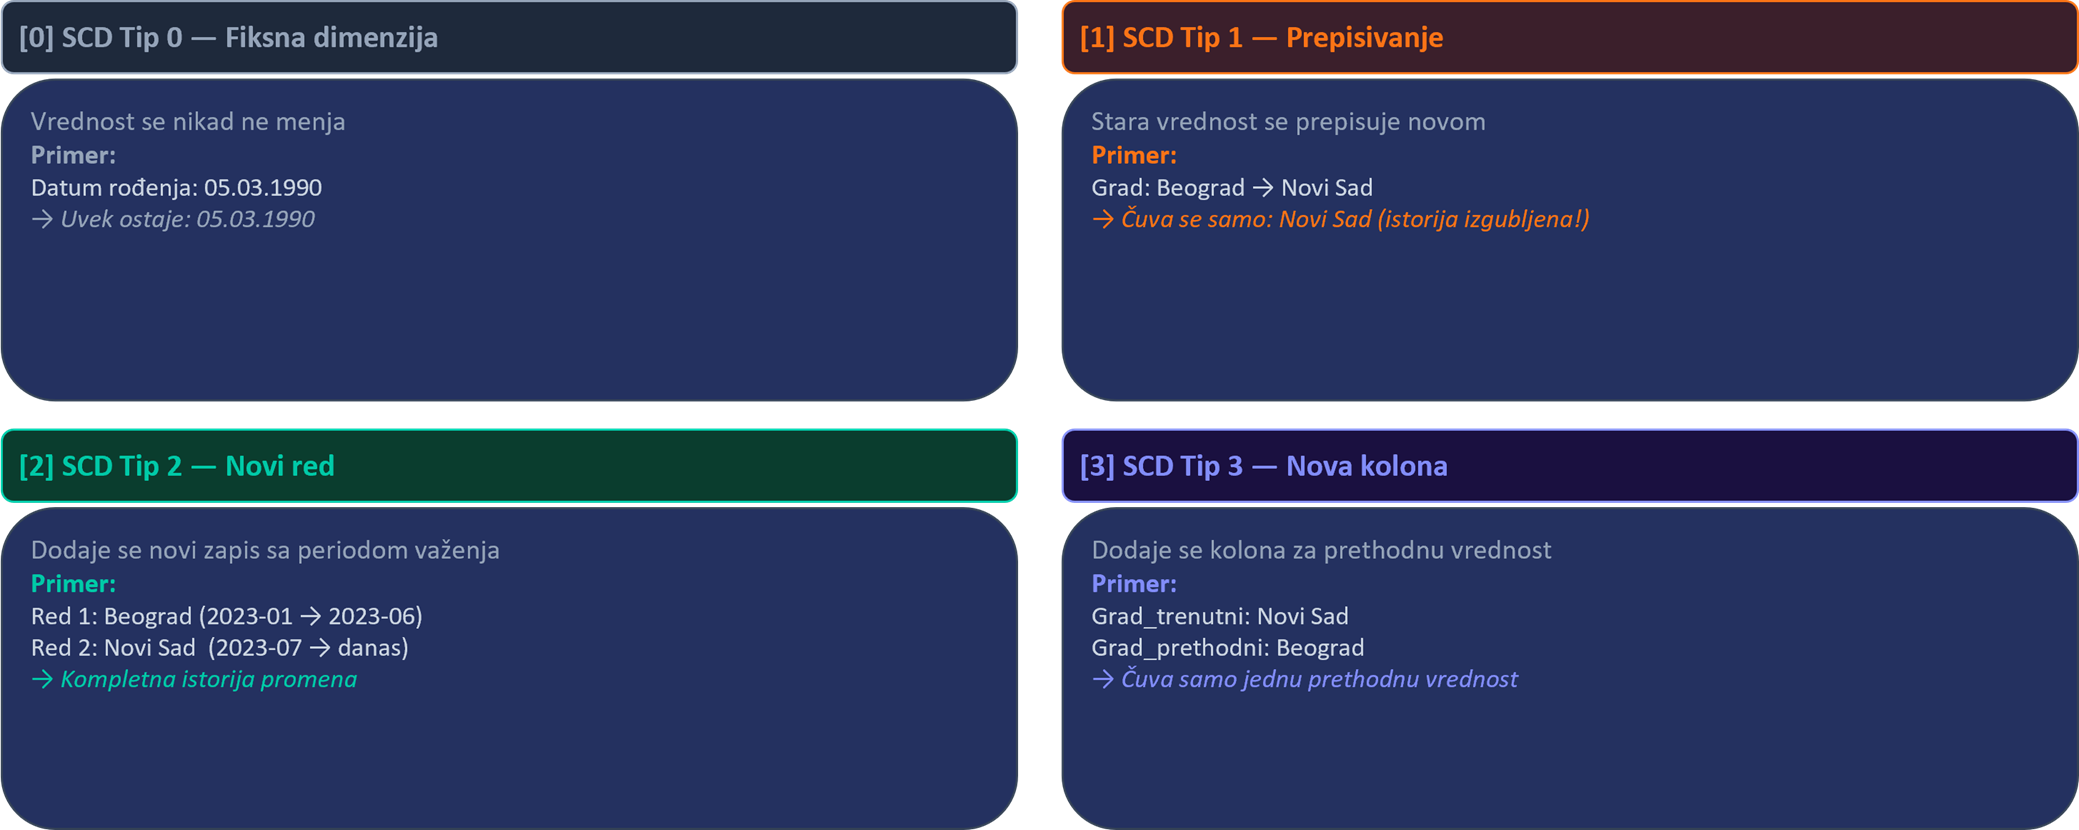
\includegraphics[width=0.85\linewidth]{slike/02/02-25.png}
    \caption{Споро мењајуће димензије (енг. slowly changing dimensions): типови 0–3, четири стратегије за руковање променом у атрибуту димензије}
    \label{fig:02-20}
\end{figure}

\textbf{\textit{SCD Type 0 — фиксна димензија.}} Атрибут се третира као непроменљив: када се једном забележи, више се никада не мења. Type 0 је прави избор за атрибуте који се заиста не могу мењати, датум рођења купца, датум прве производње производа, а погрешан избор за све остало, јер његова примена на променљив атрибут једноставно значи да складиште тихо губи кореспонденцију са стварношћу.

\textbf{\textit{SCD Type 1 — преписивање.}} Када дође до промене, постојећи ред се ажурира на лицу места; претходна вредност се губи. Type 1 је исправан само када историја није важна и када је најновија вредност једина вредност која ће складишту икада бити потребна. То је најједноставнија стратегија за имплементацију и најопаснија за примену као подразумевана, она унутар самог складишта поново уводи управо ону волатилност коју архитектура постоји да спречи. Радни пример у наставку овог одељка показује како примена Type 1 на атрибут који се користи за груписање тихо корумпира сваки историјски извештај.

\textbf{\textit{SCD Type 2 — нови ред.}} Када дође до промене, постојећи ред се затвара постављањем крајњег датума, а убацује се нови ред са новом вредношћу атрибута, отвореним крајњим датумом и новим сурогат кључем. Type 2 чува потпуну историју димензије: сваки ред носи период важења (datum\_od, datum\_do), и сваки историјски fact спојен са својом верзијом димензије преузима вредност атрибута онакву каква је била када је fact забележен. Type 2 је доминантна стратегија у пракси и стандардни избор за сваки атрибут димензије који се користи у историјској анализи (Kimball \& Ross, 2013).

\textbf{\textit{SCD Type 3 — нова колона.}} Када дође до промене, постојећи ред се ажурира на лицу места, али нова колона бележи претходну вредност. Type 3 чува тачно једно историјско стање, најновију промену, и прикладан је за атрибуте код којих корисници желе да упореде „тренутно” са „претходним”, али им није потребна пуна историја, на пример реорганизација продајне територије, где колона previous-territory подржава year-over-year извештаје током транзиције.

SCD Type 2 захтева структуру кључева која разликује верзије истог пословног ентитета, и управо ту сурогат кључ зарађује своје централно место у димензионом моделирању (Kimball \& Ross, 2013). Природни кључ је идентификатор који користе пословање и изворни системи, ID купца, SKU производа, национални идентификациони број. Природни кључ идентификује ентитет, али не разликује његове верзије: купац 1001 има један природни кључ без обзира на то да ли складиште садржи њен ред за Београд из 2021. или ред за Нови Сад из 2024.

Сурогат кључ је вештачки цео број који генерише само складиште, типично помоћу IDENTITY колоне или механизма секвенце (енг. \textit{sequence}), и који јединствено идентификује један ред у табели димензије. Свака верзија ентитета добија сопствени сурогат кључ: ред купца 1001 за Београд из 2021. може имати сурогат кључ 501, а ред за Нови Сад из 2024. сурогат кључ 502. Табеле чињеница складишта затим референцирају димензије преко сурогатног кључа, никада преко природног кључа. Резултат је да ред табеле чињеница забележен 2022. носи сурогатни кључ 501 у колони customer\_sk и спаја се са верзијом купца 1001 за Београд, што је било стварно стање купца у то време. Ред табеле чињеница забележен 2024. носи сурогатни кључ 502 и спаја се са верзијом за Нови Сад. Сваки такав ред чува се у односу на стање димензије под којим се заиста догодио.

Сурогат кључеви су независни од кључева изворних система и преживљавају њихове промене; омогућавају чланове “unknown” или “not applicable”, типично са резервисаним кључевима као што су 0 или -1, без загађивања простора природних кључева; и уједначено су целобројног типа кроз све димензије, што поједностављује спајања и индексирање. Ове секундарне предности су разлог што се сурогат кључеви препоручују чак и за димензије које нису подложне Type 2 верзионисању (Kimball \& Ross, 2013).

Претпоставимо да складиште примењује SCD Type 1 на атрибут град. Када дође до промене у јануару 2024, поље city у реду купца бива преписано са “Beograd” на “Novi Sad”; претходна вредност нестаје. Извештај о приходу по граду, написан као спајање из FACT\_SALES кроз DIM\_CUSTOMER по природном кључу и груписан по граду, сада приписује свих 580.000 RSD купчевих животних куповина Новом Саду, укључујући и 500.000 RSD који су заправо купљени док је купац живео у Београду. Ред за Београд у извештају показује нулу. Број је погрешан, и што је још горе, сам извештај је структурно неспособан да буде исправан: подаци потребни да би се историјска продаја доделила исправном граду су преписани и више нису у складишту.

\begin{figure}[h]
    \centering
    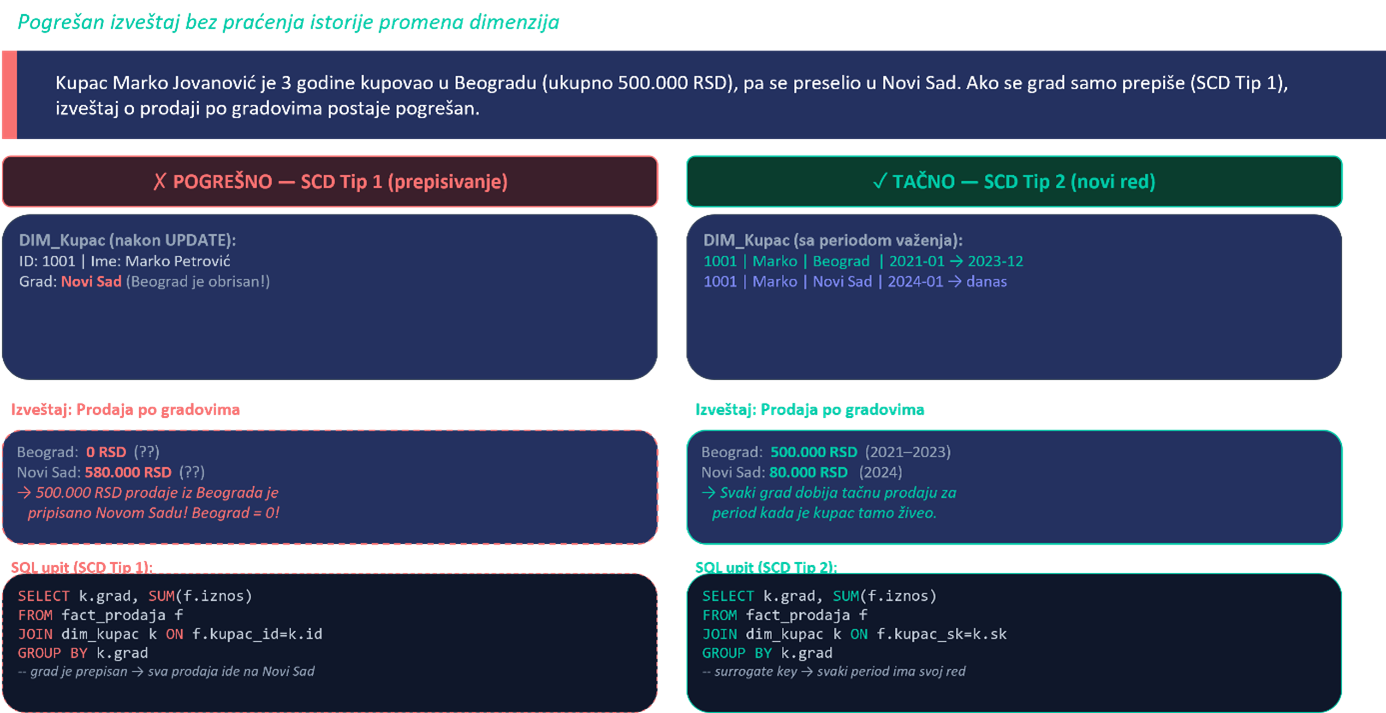
\includegraphics[width=0.85\linewidth]{slike/02/02-06.png}
    \caption{Промена града купца: Type 1 (лево) погрешно приписује историјски приход из Београда Новом Саду; Type 2 (десно) чува период важења и враћа исправан приход по граду}
    \label{fig:02-21}
\end{figure}

Претпоставимо да складиште примењује SCD Type 2. Постојећи ред димензије купца затвара се крајњим датумом 31. децембар 2023. и сурогат кључем 501; убацује се нови ред са сурогат кључем 502, новим градом Нови Сад, почетним датумом 1. јануар 2024. и отвореним крајњим датумом. Fact редови забележени између 2021. и 2023. носе customer\_sk = 501 и спајају се са верзијом за Београд; fact редови забележени од 2024. па надаље носе customer\_sk = 502 и спајају се са верзијом за Нови Сад. Исти упит прихода по граду, сада написан као спајање по сурогат кључу, враћа 500.000 RSD за Београд и 80.000 RSD за Нови Сад. Сваки град добија приход који је заиста остварен док је купац тамо живео.

Пример је мали, али поука коју даје је општа: примена SCD Type 1 на атрибут који се користи за груписање тихо корумпира сваки историјски извештај који по њему групише, а корупција се не може открити из самог извештаја, бројеви се сабирају у исправан укупан збир, само су погрешно распоређени по групама. Избор SCD стратегије стога није технички детаљ већ суштинска одлука моделирања и мора бити донет намерно за сваки атрибут сваке димензије коју складиште излаже за груписање.

\subsubsection{Димензионо моделовање}
Четири својства из §§2.2.3.1–2.2.3.5 одређују шта складиште података мора бити; она не одређују како су његове табеле распоређене. Зато, ова секција следи препоруке Кимбала и Роса (Kimball \& Ross, 2013) и усваја димензионо моделирање као радни дизајн шеме. Димензионо моделирање организује складиште у две врсте табела, табеле чињеница и табеле димензија, и прописује мали број канонских образаца шема који их комбинују. Ова секција уводи те две врсте табела, разрађује четири канонска обрасца, једнотабеларни, звездасти, пахуљасти и галаксијски, и третира грануларност као дизајнерску одлуку од које зависи остатак шеме.

\paragraph{Чињенице и димензије}
Табела чињеница бележи мерења која произилазе из пословног процеса: продату количину и остварени приход за сваку ставку сваке поруџбине, ниво залиха за сваки производ у сваком складишту сваког дана, исплаћену зараду сваком запосленом у сваком платном периоду и оцену студента на испиту. Редови табеле чињеница су догађаји или стања; колоне су нумеричке мере повезане са сваким од њих (Kimball \& Ross, 2013). 

Мере у табелама чињеница типично су \textbf{\textit{адитивне}}: количине и износи природно се сабирају преко било које комбинације димензија. Неке мере су \textbf{\textit{полуадитивне}}, ниво залиха не може се сабирати преко дана али може преко складишта, а неке су \textbf{\textit{неадитивне}}, као што су јединична цена или просечан однос. У већини случајева мерења морају бити представљена као нумеричке вредности. Међутим, постоје случајеви када се мерења могу израчунати на основу категоријалних вредности. На пример: број, или различит број, купаца. Овде се могу користити категоријалне вредности, нпр. CustomerID, али је агрегатна функција count, односно count distinct. И други примери су уобичајени: број различитих производа купљених по поруџбини, број продавница које су имале артикал на стању у одређеној недељи, број јединствених посетилаца веб-странице или број запослених који су завршили курс обуке. Агрегатне функције које се примењују над табелама чињеница стога су разноврсне. 

Нумеричке мере се најчешће сабирају (SUM) или усредњавају (AVG); полуадитивне мере се типично сабирају преко неких димензија, а усредњавају или узимају у одређеном тренутку преко других, ниво залиха сабран преко складишта али усредњен преко дана, или прочитан на крају месеца. Поред SUM, AVG, COUNT и COUNT DISTINCT, уобичајене функције укључују MIN и MAX, највећи износ фактуре у кварталу, најранији датум поруџбине за купца, MEDIAN и процентилне агрегате (енг. \textbf{\textit{percentile aggregates}}), медијалну вредност поруџбине, 95. перцентил времена испоруке, STDDEV и VAR, волатилност дневне продаје, и односне мере (енг. \textbf{\textit{ratio measures}}) изведене из два основна збира, као што су бруто маржа, приход минус трошак подељен приходом, и стопа конверзије, број поруџбина подељен бројем сесија. Избор агрегатне функције је својство саме мере, а не упита, и мора бити декларисан у семантичком слоју тако да BI алати доследно агрегирају кроз извештаје.

Табела димензије бележи контексте, односно димензије у односу на које се табеле чињеница анализирају: купца који је извршио поруџбину, производ који је продат, датум када је продаја извршена и географију у којој купац живи. Редови табеле димензије су ентитети или чланови; колоне су атрибути тих ентитета по којима корисник жели да филтрира, групише или врши продубљивање увида (енг. \textit{drill-down}). Димензије су типично широке, имају много атрибута и плитке су, односно садрже релативно мало редова у поређењу са табелама чињеница, а денормализоване су тако да се регион, држава и континент појављују као колоне у DIM\_GEOGRAPHY, а не као засебне нормализоване табеле. Тако је упиту потребно само једно спајање са табелом чињеница да би преузео било који атрибут контекста.

Табеле чињеница и табеле димензија повезане су страним кључевима на сурогат кључеве: сваки ред у FACT\_SALES носи customer\_sk, product\_sk, date\_sk и geography\_sk, а сваки од њих спаја се са одговарајућом табелом димензије по њеном сурогат кључу. Дисциплина ограничавања страних кључева табеле чињеница на сурогат кључеве и денормализације сваке димензије у једну широку табелу јесте оно што димензионим шемама даје њихове аналитичке перформансе и читљивост за BI алате.

\paragraph{Грануларност}
Пре него што се дефинишу димензије и табеле чињеница, дизајнер мора да одговори на питање: шта представља један ред табеле чињеница? Одговор на ово питање дефинише грануларност (енг. \textit{grain}), односно ниво детаља података, а Кимбал и Рос (Kimball \& Ross, 2013) стављају је у средиште процеса дизајна: најпре се декларише грануларност, затим се идентификују димензије које су с њом конзистентне, па тек онда мере које су на том нивоу грануларности адитивне.

Грануларност исказана у једној реченици, „један ред по ставци сваке фактуре”, „један ред по пакету скенираном на сваком кораку сваке пошиљке”, „један ред по минуту сваког позива”, дисциплинује сваки наредни дизајнерски избор.

Избор грануларности је компромис. Најфинија (највиши ниво) могућа грануларност, један ред по атомском пословном догађају, чува сваки детаљ, али производи највеће табеле чињеница и најспорије упите. Грубља (нижи ниво) грануларност, дневни сажеци уместо појединачних трансакција, месечни сажеци уместо дневних, смањује број редова и убрзава упите по цену детаља. Пример на наредној слици репродукује пример детаљних записа о позивима (енг. \textbf{\textit{call-detail records}}) из изворне презентације: телекомуникациони оператор може чувати појединачне записе о позивима (Слика~\ref{fig:02-22}) (200 редова, 4.000 бајтова по кориснику месечно) на једној крајности и један месечни сажет ред (један ред, 200 бајтова по кориснику месечно) на другој. Сажетак је двадесет пута ефикаснији у простору и бржи за упите, али не може одговорити на питања о појединачним позивима.

\begin{figure}[h]
    \centering
    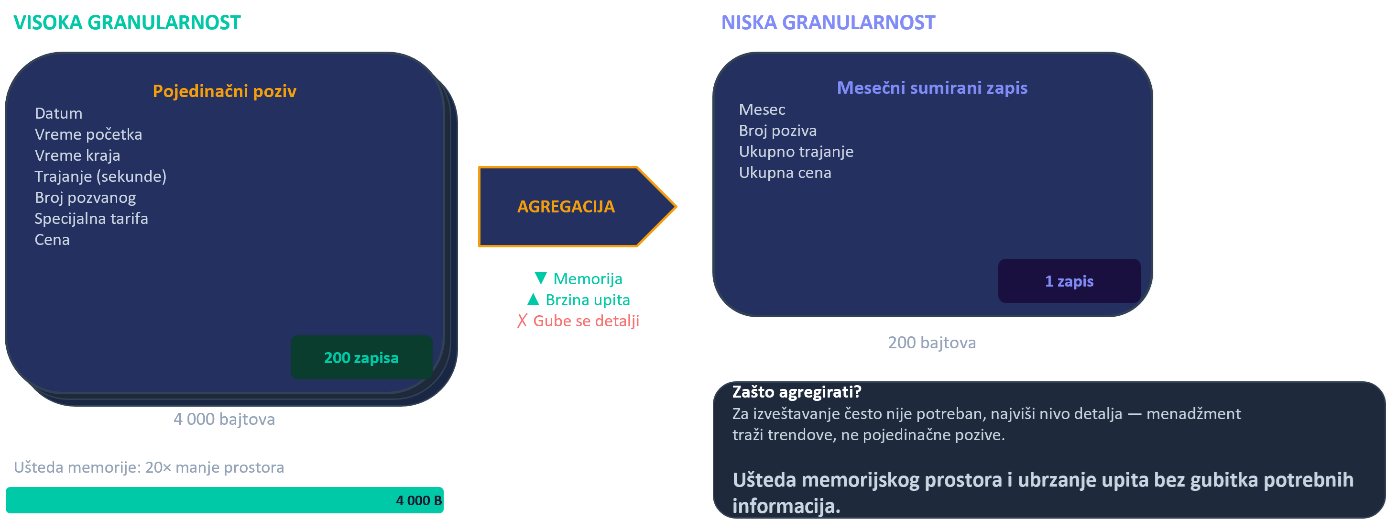
\includegraphics[width=0.85\linewidth]{slike/02/02-12.png}
    \caption{Компромис грануларности: атомски записи детаља позива (енг. call-detail records) насупрот месечним сажетим редовима}
    \label{fig:02-22}
\end{figure}

У пракси, складишта чувају најфинији доступан ниво грануларности и ослањају се на агрегацију како би по потреби произвела грубље приказе (Kimball \& Ross, 2013). Унапред израчунате агрегатне табеле, дневни сажетак изведен из табеле чињеница на нивоу трансакције, месечни сажетак изведен из дневног, убрзавају најчешће упите, док атомска табела чињеница остаје доступна за непредвиђена питања. OLAP коцка из §2.2.3.7 представља генерализацију ове идеје: она унапред израчунава агрегације преко сваке релевантне комбинације нивоа димензија.

\paragraph{Схеме складишта података}
Четири схеме складишта података димензионим моделирањем. Они се разликују по томе како мењају редундантност за перформансе упита и колико пословних процеса могу да обухвате.

\textbf{\textit{Једнотабеларна шема}} (енг. \textit{flat schema}). Сви атрибути, чињенице и свака контекстуална колона чувају се у једној денормализованој табели. Упити не захтевају спајања и враћају веома брзе резултате, али је табела веома редундантна, регион купца се понавља у сваком продајном реду, трошак складиштења је висок, а свако ажурирање контекстуалног атрибута захтева дотицање сваког реда чињенице. Једнотабеларна шема погодна је за мале, једноставне скупове података и за неке имплементације колонарних складишта где се редундантност добро компресује; она не скалира на складишта на нивоу предузећа.

\begin{figure}[h]
    \centering
    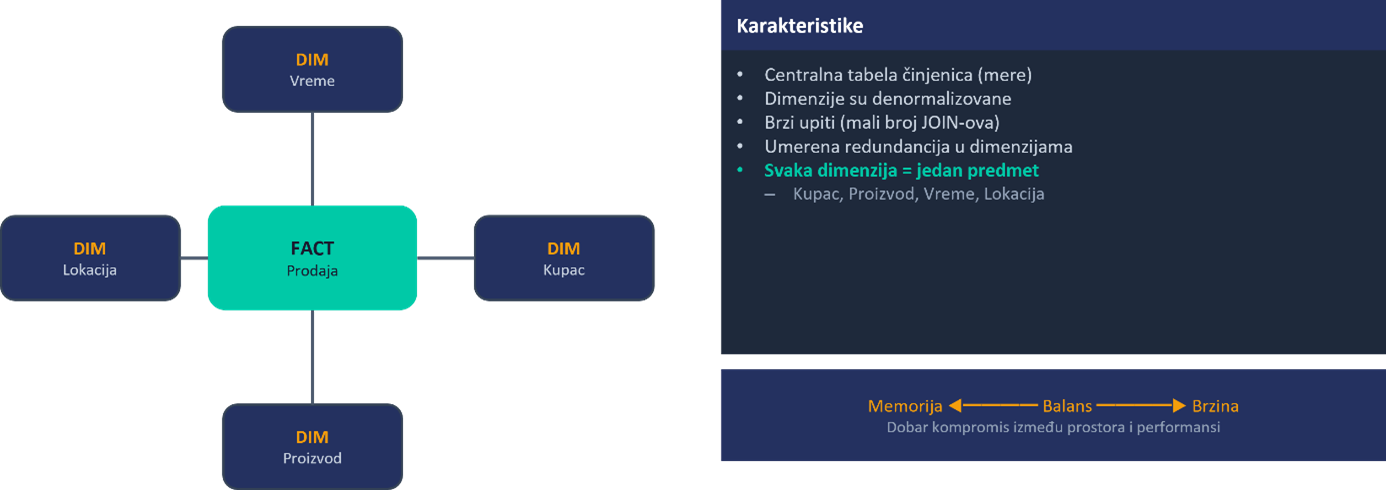
\includegraphics[width=0.85\linewidth]{slike/02/02-10.png}
    \caption{Звездаста шема (енг. star schema): централна fact табела окружена денормализованим димензијама}
    \label{fig:02-23}
\end{figure}

Звездаста шема (енг. star schema). Табела чињеница је повезана са денормализованим димензионим табелама на једном нивоу спајања, при чему свака димензија има један примарни кључ који се као страни кључ налази у табели чињеница. Иако су димензионе табеле денормализоване, шема заузима драстично мање складишног простора него једнотабеларна — контекстуални атрибути се не понављају у сваком реду чињенице, већ се спајају по потреби. Извештавање је нешто спорије од једнотабеларне шеме због неопходних спајања, али је и даље брзо: модел остаје једноставан за разумевање и оптимизацију, па је звездаста шема најчешћи избор у складиштима података на нивоу предузећа (Kimball \& Ross, 2013).

\begin{figure}[h]
    \centering
    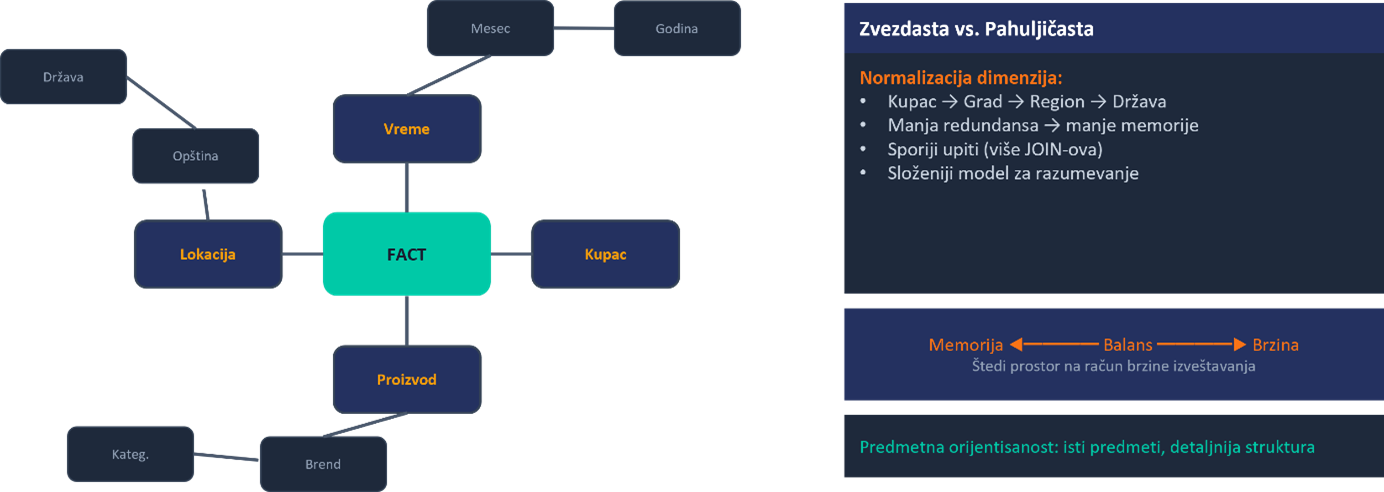
\includegraphics[width=0.85\linewidth]{slike/02/02-14.png}
    \caption{Пахуљаста шема (енг. snowflake schema): димензије нормализоване у поддимензије, чиме се смањује редундантност по цену додатних спајања}
    \label{fig:02-24}
\end{figure}

Пахуљаста шема (енг. snowflake schema). Димензионе табеле (једна или више њих) су нормализоване, обично до 3NF, тако да се хијерархијски атрибути (нпр. град → регион → држава, производ → подкатегорија → категорија) разлажу у засебне поддимензионе табеле повезане преко страних кључева. Редундантност се додатно смањује и описни атрибути се одржавају на једном месту, али упити захтевају више спајања, па је извештавање спорије од звездасте шеме. Пахуљаста шема се користи када су димензионе хијерархије стабилне, када је заузеће складишног простора критично или када се захтева строг интегритет описних атрибута.

\begin{figure}[h]
    \centering
    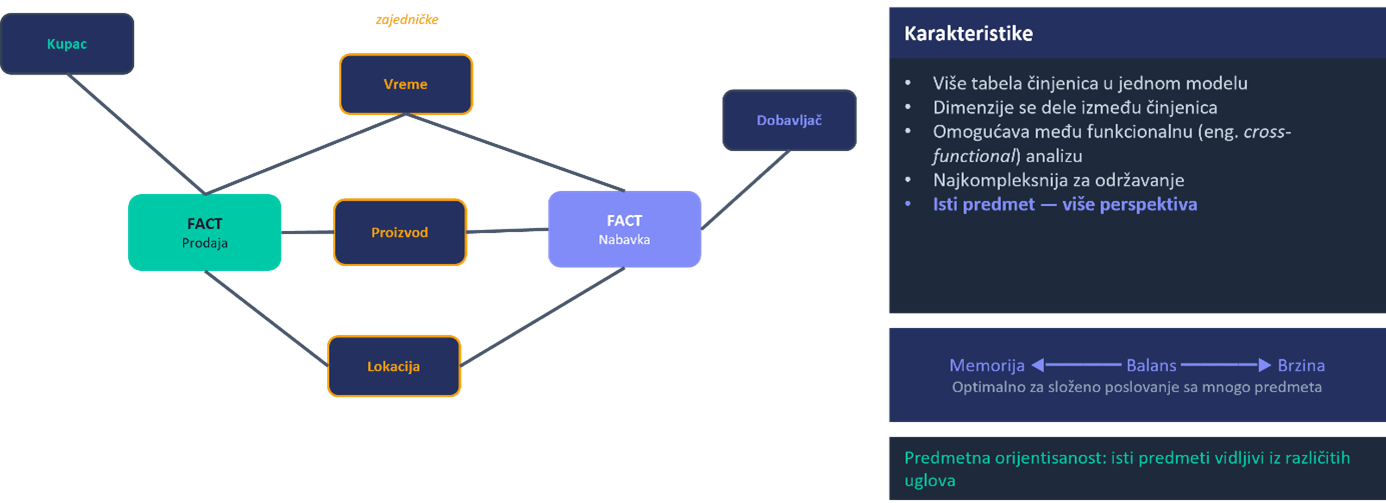
\includegraphics[width=0.85\linewidth]{slike/02/02-19.png}
    \caption{Галаксијска шема (енг. galaxy schema, fact constellation): више fact табела које деле заједнички скуп усаглашених димензија (енг. conformed dimensions)}
    \label{fig:02-25}
\end{figure}

Галаксијска шема (енг. galaxy schema, fact constellation). Више табела чињеница из различитих пословних процеса дели заједнички скуп усаглашених димензија (енг. conformed dimensions), па се иста димензиона табела (нпр. време, купац, производ) користи за више независних мерења. Шема омогућава унакрсну анализу процеса — на пример, поређење продаје и рекламација по истим димензијама — али је сложенија за пројектовање и одржавање јер захтева доследну дефиницију усаглашених димензија на нивоу целог складишта. Користи се у зрелим складиштима података на нивоу предузећа која покривају више међусобно повезаних пословних процеса (Kimball \& Ross, 2013).

\subsubsection{OLAP коцке и пивот табеле}
Димензионе шеме чине аналитичке упите брзим; OLAP коцке их чине тренутним. Ова секција уводи вишедимензиону структуру која је постала стандардни аналитички слој складишта података, разликује три архитектуре складиштења путем којих се она имплементира и затвара круг са пивот табелом, формално, клијентом коцке, која проширује интерактивне аналитичке технике разрађене у §2.1.8. 

\paragraph{OLAP коцка}
Термин аналитичка обрада на мрежи (енг. \textit{online analytical processing}, OLAP) увели су Код, Код и Сали (Codd, Codd, \& Salley, 1993) како би разликовали аналитичко радно оптерећење, вишедимензионо, агрегирајуће и истраживачко, од трансакционог радног оптерећења (OLTP) оперативних система. OLAP коцка је структура података која подржава ово радно оптерећење (Слика~\ref{fig:02-26}): вишедимензиони низ у којем свака димензија одговара једној аналитичкој оси (време, производ, географија, купац), а свака ћелија на пресеку чланова димензија садржи агрегирану меру (збир прихода, број поруџбина, просечну маржу). Код, Код и Сали (Codd, Codd, \& Salley, 1993) и Чаудхури и Дајал (Chaudhuri \& Dayal, 1997) пружају темељне описе; Кимбал и Рос (Kimball \& Ross, 2013) третирају коцку као природну, за читање оптимизовану пројекцију звездасте или галаксијске шеме.

Коцка се гради из табеле чињеница унапред израчунавањем сваке агрегације која би могла бити од интереса дуж димензија коцке: укупан приход по години, по кварталу, по месецу и по дану; по држави, по региону и по граду; и по свакој комбинацији ових. Агрегације се чувају у индексираној структури која подржава проналажење по координатама димензија. Упит који тражи приход по граду за 2024. не скенира табелу чињеница и не израчунава SUM и GROUP BY у реалном времену; он врши индексирано проналажење унапред израчунате ћелије на координати (Time = 2024, Geography = сваки град) и одмах враћа одговор. Тамо где би SQL упит над табелом чињеница од милиона редова могао трајати од пет до тридесет секунди, коцка враћа резултат за мање од секунде (Chaudhuri \& Dayal, 1997).

Најједноставнији начин да се коцка интуитивно разуме јесте пример са три димензије: време × производ × регион. Замислимо да једна ћелија коцке садржи укупан приход за комбинацију „Q1 2025, млечни производи, Београд”. Ако аналитичар фиксира време на 2025. годину и посматра само производе и регионе, извео је пресек коцке (енг. \textbf{\textit{slice}}). Ако затим ограничи и време на први квартал и регион на Србију север, добија ужи подскуп (енг. \textbf{\textit{dice}}). Ако из приказа „2025” пређе на „Q1, Q2, Q3, Q4”, изводи продубљивање увида (енг. \textbf{\textit{drill-down}}) дуж временске хијерархије; ако се из месеци врати на године, ради сажимање на виши ниво (енг. \textbf{\textit{roll-up}}). Управо ове операције стоје иза утиска да се пивот табела или контролна табла „одмах” преобликује када корисник промени ниво посматрања.

\begin{figure}[h]
    \centering
    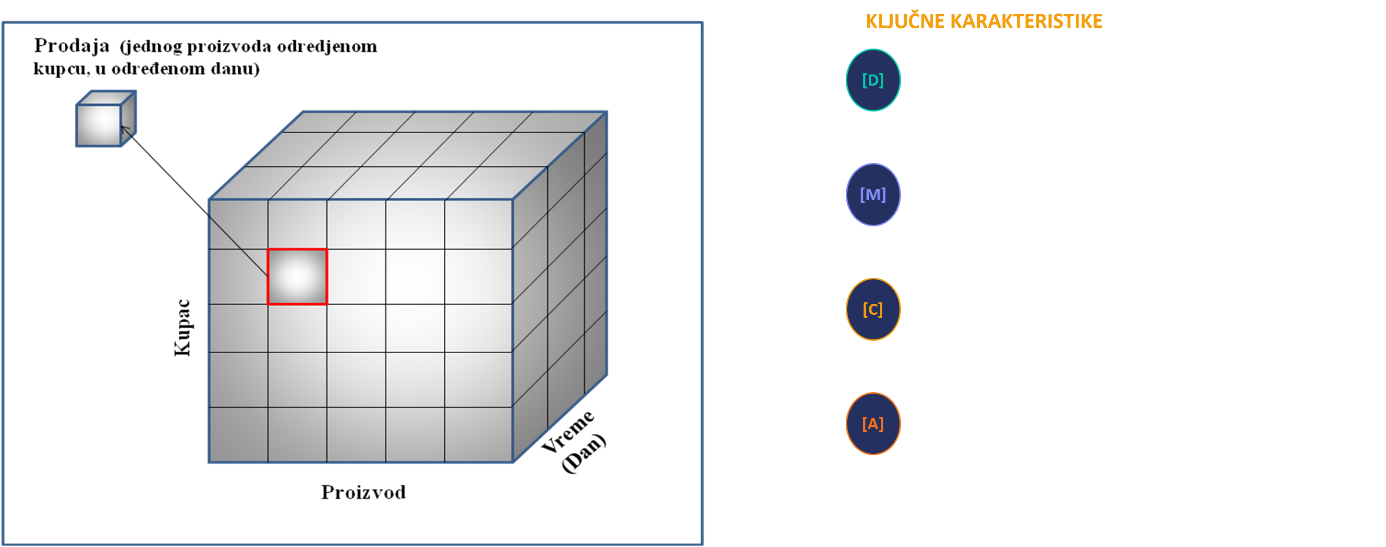
\includegraphics[width=0.85\linewidth]{slike/02/02-08.png}
    \caption{OLAP коцка: вишедимензиона структура у којој свака ћелија садржи унапред израчунату агрегирану меру}
    \label{fig:02-26}
\end{figure}

Стандардне аналитичке операције над коцком су:

\begin{itemize}
  \item \textbf{\textit{пресек}} (енг. \textit{slice}; фиксирање једне димензије на вредност, нпр. Time = 2024),
  \item \textbf{\textit{подскуп}} (енг. \textit{dice}; фиксирање више димензија, нпр. Time = 2024 и Region = Vojvodina),
  \item \textbf{\textit{продубљивање увида}} (енг. \textit{drill-down}; спуштање низ хијерархију, нпр. са године на квартал па на месец),
  \item \textbf{\textit{сажимање на виши ниво}} (енг. \textit{roll-up}; пењање уз хијерархију), и
  \item \textbf{\textit{ротација}} (енг. \textit{pivot}; излагање различитог пара димензија у унакрсној табелацији).
\end{itemize}
Свака од ових операција директно одговара радњи коју корисник предузима на контролној табли или пивот табели, због чега се коцка и пивот табела тако природно уклапају.

\paragraph{Пивот табела као OLAP клијент}
Пивот табела, аналитичарев инструмент за унакрсно табелирање мера кроз две или више димензија, допуњује интерактивне технике из §2.1.8. Када је коцка успостављена, пивот табела добија своју формалну улогу: она је клијент OLAP коцке. Корисников избор редова, колона, филтера и мера спецификује упит у координатном простору коцке, коцка враћа претходно агрегиране ћелије које одговарају том упиту, а пивот табела их приказује као унакрсну табелацију. Када корисник превуче нову димензију у област редова, пивот табела издаје нови упит коцки на новом нивоу грануларности; када корисник прошири хијерархију, пивот табела издаје упит за продубљивање увида (енг. \textbf{\textit{drill-down}}). Интеракција коју аналитичар доживљава као тренутну, испод површине је низ индексираних претрага коцке.

Овај однос има практичне последице. Пивот табела која ради директно над радним листом изворних података ограничена је лимитима радног листа — Excel-ово ограничење редова је приближно милион по листу — и меморијским агрегирајућим механизмом табеларног калкулатора. Насупрот томе, пивот табела повезана са OLAP коцком ради над претходно агрегираним ћелијама које се чувају на серверу и ограничена је величином коцке, а не величином табеларног листа. Excel пивот табеле могу бити подешене да користе Analysis Services коцке као извор података; кориснички интерфејс је познати табеларни калкулатор, али су упити MDX (Multidimensional Expressions, стандардни језик упита за OLAP коцке), а не SQL, и обим података се протеже до милијарди редова чињеница.

Читалац стога може задржати интуицију да је пивот табела алат за сечење, груписање и филтрирање, тесно повезан са интерактивним техникама из §2.1.8, и томе додати архитектонску слику коју је овај одељак развио. Пивот табела припада корисничком слоју (енг. \textbf{\textit{front end}}); OLAP коцка је аналитички слој оптимизован за читање који стоји иза ње; коцка се гради из звездасте или галаксијске шеме (енг. \textit{star} или \textit{galaxy schema}); шема се пуни из изворних система ETL процесом; и целокупан овај распоред постоји зато што OLTP системи описани у §2.2.2 не могу, сами по себи, да одговоре на питања која менаџери постављају својим подацима.

\paragraph{MOLAP, ROLAP и HOLAP}
Три имплементационе архитектуре доминирају, а разликују се по томе где се подаци коцке чувају и како им се приступа (Chaudhuri \& Dayal, 1997).

Multidimensional OLAP (MOLAP) смешта коцку у наменски изграђену вишедимензионалну базу података која материјализује агрегације у компресованој, индексираној структури. Упити су изузетно брзи зато што се одговори читају директно из индексираних ћелија; цена су велики иницијални захтеви за складиштењем и дуготрајан процес изградње коцке када се основне чињенице промене. Microsoft Analysis Services и Oracle Essbase су репрезентативни MOLAP механизми.

Relational OLAP (ROLAP) чува коцку као скуп табела у релационој бази података — типично у истом складишту које садржи основне чињенице — и одговара на упите над коцком тако што их преводи у SQL са одговарајућим агрегацијама. Складиштење је ефикасније јер агрегације нису у потпуности унапред материјализоване, а архитектура се природно скалира на веома велике табеле чињеница; цена су спорији појединачни упити зато што SQL агрегација мора да се изврши у тренутку упита, чак и када јој помажу aggregate tables и column-store индекси. SAP BW и MicroStrategy су репрезентативне ROLAP платформе.

Hybrid OLAP (HOLAP) комбинује ова два приступа: агрегиране вредности се чувају у вишедимензионалној структури ради брзих упита сажимања на виши ниво (енг. \textbf{\textit{roll-up}}), док основни детаљни редови остају у релационом складишту ради продубљивања увида (енг. \textbf{\textit{drill-down}}) до атомског нивоа грануларности. HOLAP је подразумевани режим већине савремених OLAP механизама јер обухвата већину MOLAP перформанси упита уз већину ROLAP економичности складиштења. Компромиси између ове три архитектуре могу се сажети овако: брзина упита иде редом MOLAP > HOLAP > ROLAP, док и трошак складиштења следи исти редослед. Избор зависи од величине табела чињеница, захтева за кашњењем BI корисничког слоја (енг. \textit{front end}) и расположивог буџета за рачунарске ресурсе и складиштење.

\begin{figure}[h]
    \centering
    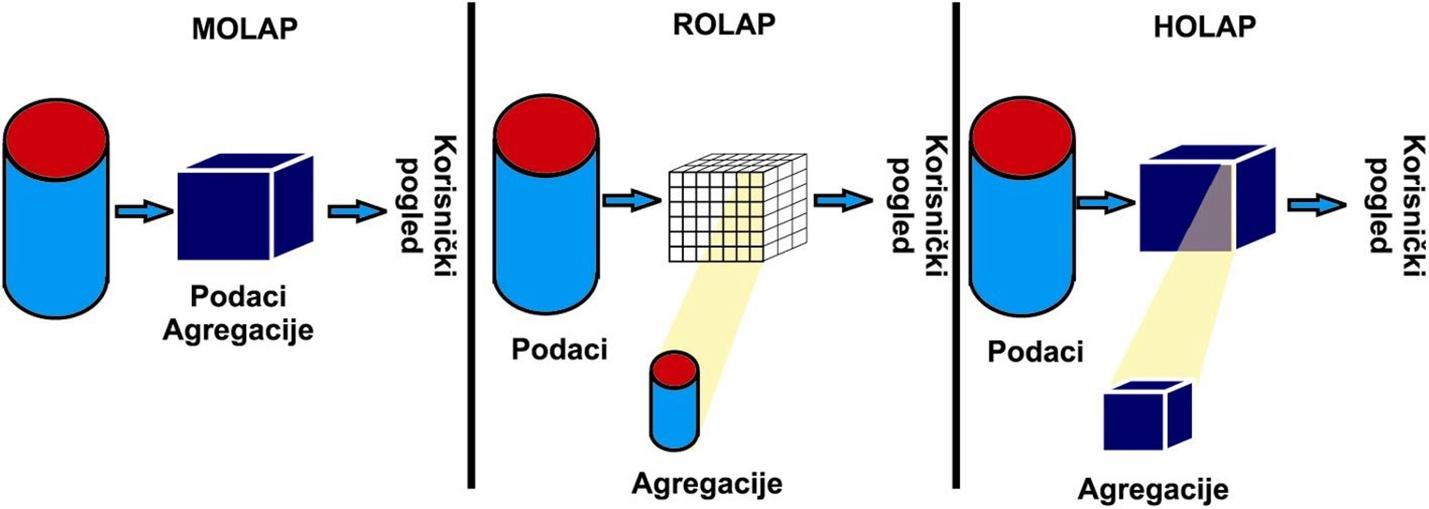
\includegraphics[width=0.85\linewidth]{slike/02/02-04.jpg}
    \caption{Типови OLAP коцки: MOLAP, HOLAP и ROLAP}
    \label{fig:02-27}
\end{figure}

\subsection{Изградња складишта података}
У овој секцији ће бити разматран развој складишта података. Две методологије — повезане са Вилијамом Инмоном (William Inmon) и Ралфом Кимбалом (Ralph Kimball) — доминирају овом облашћу већ три деценије. Иако наизглед супротстављене, ове методологије заправо имају исте циљеве, али их остварују на различите начине у зависности од контекста потреба за аналитичким захтевима.

\subsubsection{EDW и центри података}
\textbf{\textit{Enterprise data warehouse}} (EDW) је централизовано аналитичко складиште које интегрише структуриране податке из више изворних система широм организације и подржава извештавање и аналитику за предузеће у целини. Оно задовољава све четири Инмонове особине (§2.2.3.1) и служи, језиком који се понекад користи у пракси, као „single source of truth for management decisions”: један консолидован скуп података над којим се свако одељенско или међуфункционално питање може доследно решити (Inmon, 2005).

\textbf{\textit{Центар података}} (енг. \textit{data mart}) је тематски подскуп складишта, усмерен на једну пословну функцију — продају, финансије, људске ресурсе, маркетинг, CEO, CTO итд. — и оптимизован за упите које корисници те функције заиста извршавају (Kimball \& Ross, 2013). Продајни центар података садржи димензије и чињенице релевантне за анализу продаје (FACT\_SALES, DIM\_DATE, DIM\_PRODUCT, DIM\_CUSTOMER, DIM\_GEOGRAPHY) и подржава извештаје као што су приход по региону, најпродаванији производи и учинак продајних представника. Финансијски центар података садржи FACT\_GENERAL\_LEDGER и FACT\_BUDGET уз DIM\_ACCOUNT, DIM\_COST\_CENTER, DIM\_DATE и DIM\_LEGAL\_ENTITY, и подржава извештаје као што су поређење буџета и остварења по центру трошка, месечни P\&L и трендови обртног капитала. Производни центар података садржи FACT\_PRODUCTION\_OUTPUT и FACT\_DOWNTIME уз DIM\_PLANT, DIM\_PRODUCTION\_LINE, DIM\_PRODUCT, DIM\_SHIFT и DIM\_DATE, и подржава извештаје као што су број произведених јединица по смени, стопа шкарта по линији и узроци застоја по погону. Сваки центар података обликован је питањима која његови корисници заиста постављају.

Мартови постоје из четири разлога:

\begin{itemize}
  \item Прво, они нуде брже перформансе упита за своју циљну тематску област јер садрже само релевантне податке и могу бити уско подешени.
  \item Друго, они дају одељењу контролу над сопственим моделом података — дефиницијама мера, грануларношћу, SCD политикама — без потребе за сагласношћу читаве организације.
  \item Треће, лакши су за одржавање од једног монолитног складишта, јер се промене у једном марту не преносе ван његовог опсега.
  \item Четврто, поједностављују безбедност и контролу приступа: сваки март је ограничен на једну пословну функцију, па се привилегије засноване на улогама могу додељивати на нивоу марта — корисници финансија приступају финансијском марту, HR корисници HR марту — без излагања података ван њиховог домена.
\end{itemize}
Ово покреће основно питање: како су EDW и мартови међусобно повезани? Могућа су два одговора. По Инмоновом схватању, EDW се гради прво као јединствено интегрисано складиште, а мартови се из њега изводе као тематски усмерени подскупови. По Кимбаловом схватању, мартови се граде прво, један пословни процес у датом тренутку, и заједно чине складиште — повезани заједничким (conformed) димензијама. Ова два виђења воде ка две различите методологије, два различита артефакта планирања и два различита низа корака рада, који се развијају у наредна два пододељка.

\subsubsection{Инмонов приступ}
Инмонов приступ полази од идеје да се најпре изгради једно централно складиште за целу организацију, а да се тек после из њега изводе ужи центри података за поједина одељења (Inmon, 2005; Inmon, Strauss, \& Neushloss, 2008). Једноставно речено: прво се прави велика, заједничка основа, па се из ње праве специјализовани прикази за продају, финансије, људске ресурсе и друге функције.

Суштина овог приступа је у томе што се интеграција ради рано и централизовано. Предност је јасна: ако сви каснији мартови настају из истог централног модела, онда је лакше одржати доследност између њих. Мана је такође јасна: потребно је више времена и договора пре него што корисници виде прве конкретне резултате.

Предности овог приступа следе непосредно. Доследност између мартова загарантована је конструкцијом, а не дисциплином. Интеграциони слој у 3NF-у прихвата промене шеме и нове изворне системе без потребе за редизајном мартова, јер су мартови пројекције, а не примарна складишта. Могућност ревизије је снажна, јер интеграциони слој при сваком учитавању бележи пуно интегрисано стање пословања. Слабости су подједнако непосредне. Време до прве испоруке је дуго, јер се пословању ништа не испоручује док се модел на нивоу предузећа не изгради и из њега не изведе бар један март. Методологија је осетљива на почетни трошак моделовања: лоше процењен модел скупо је ревидирати. Уз то, овај приступ је слабо прилагођен организацијама чији се пословни процеси мењају брже од циклуса изградње складишта (Kimball \& Ross, 2013, ch. 1).

\begin{figure}[h]
    \centering
    
\includegraphics[width=0.85\linewidth]{slike/02/02-16.png}
    \caption{Инмонова архитектура одозго надоле (енг. top-down): изворни системи напајају ETL процес који учитава нормализовано 3NF складиште на нивоу предузећа (енг. enterprise data warehouse)}
    \label{fig:02-28}
\end{figure}

\subsubsection{Кимбалов приступ}
Кимбалов приступ иде обрнутим редом: најпре се граде појединачни центри података, један по један, а они заједно временом чине шире складиште (Kimball \& Ross, 2013; Kimball, Ross, Thornthwaite, Mundy, \& Becker, 2008). Уместо једног великог централизованог модела на самом почетку, нагласак је на томе да се брже испоруче конкретна решења за поједине пословне потребе. Да би такви центри ипак могли да раде заједно, деле исте кључне димензије, на пример датум, производ или купца.

\begin{figure}[h]
    \centering
    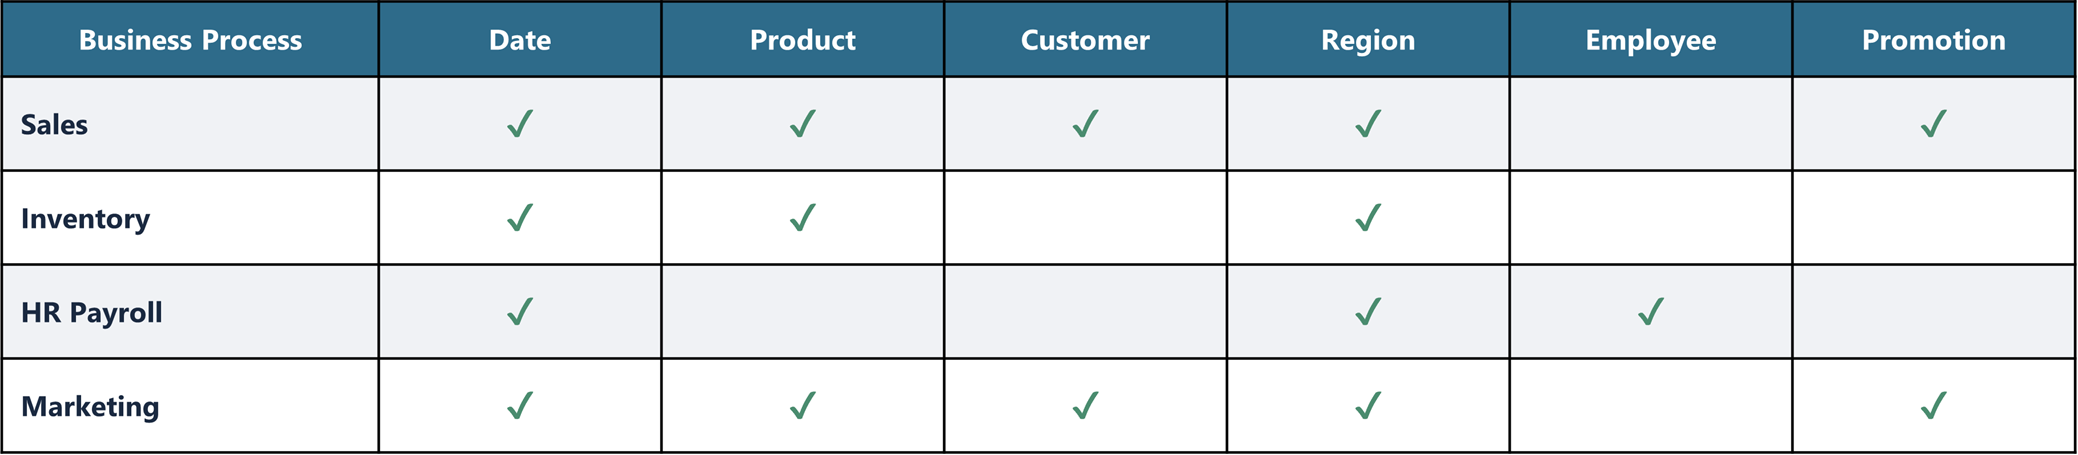
\includegraphics[width=0.85\linewidth]{slike/02/02-03.png}
    \caption{Кимбалова сабирничка матрица (енг. bus matrix): редови су пословни процеси, колоне су усаглашене димензије (енг. conformed dimensions)}
    \label{fig:02-29}
\end{figure}

Практичан алат за планирање у овом приступу јесте сабирничка матрица. Њена идеја је једноставна: у једној табели се бележи који пословни процеси користе које заједничке димензије. Тако тим лакше види шта може да се гради прво и које делове модела више мартова морају делити ако желимо да бројеви касније остану упоредиви.

Архитектура која из тога настаје назива се Кимбалова сабирница (енг. \textit{Kimball bus}): скуп димензионих мартова повезаних кичмом усаглашених димензија (енг. \textit{conformed dimensions}). Сабирница није засебна физичка структура већ дизајнерска дисциплина — мартови су физички одвојене табеле чињеница које се једноставно референцирају на идентично дефинисане димензионе табеле. План увођења мартова илустрован у изворној презентацији је типичан: Фаза 1 гради продајни март, са DIM\_DATE, DIM\_PRODUCT, DIM\_CUSTOMER и DIM\_GEOGRAPHY као усаглашеним димензијама; Фаза 2 гради финансијски март, поново користећи DIM\_DATE, DIM\_CUSTOMER и DIM\_GEOGRAPHY и додајући DIM\_ACCOUNT и DIM\_COST\_CENTER; Фаза 3 гради март људских ресурса, поново користећи DIM\_DATE и DIM\_GEOGRAPHY и додајући DIM\_EMPLOYEE и DIM\_DEPARTMENT. Редослед је вођен пословним приоритетом и зависношћу мартова од већ изграђених усаглашених димензија.

Мини-пример показује зашто су усаглашене димензије суштинске. Замислимо два марта: продајни март, чија табела чињеница бележи приход, количину и број трансакција, и маркетиншки март, чија табела чињеница бележи трошак кампање, број приказа и број кликова. Ако оба марта деле исте DIM\_DATE и DIM\_CUSTOMER табеле, аналитичар може да постави питање: колики је приход по сегменту купаца у месецима у којима је маркетиншка потрошња расла? Одговор је могућ само ако „месец” и „сегмент купца” значе исто у оба марта. Ако продаја користи сопствену верзију датума и сопствену поделу купаца, а маркетинг неку другу, поређење престаје да буде поуздано. Зато Кимбалова архитектура не тврди само да мартови треба да постоје, већ да морају бити повезани кроз исте димензије ако желимо интегрисано аналитичко окружење.

Предности овог приступа су обрнуте Инмоновим слабостима. Време до прве испоруке је кратко, јер се сваки март гради и уводи независно, а први март је у рукама корисника за неколико месеци, а не година. Итеративни ритам је боље прилагођен организацијама чији се приоритети мењају. Димензиона шема је читљива пословним корисницима и BI алатима, што и смањује терет обуке корисника и убрзава изградњу контролних табли и извештаја.

Слабости су обрнуте Инмоновим предностима. Доследност између мартова постиже се дисциплином, а не конструкцијом: ако је управљање усаглашеним димензијама слабо, два марта могу се разићи, а складиште губи своју интегративну улогу. Упити кроз процесе који обухватају више мартова зависе од тога да кључеви усаглашених димензија буду идентични у свима њима, што захтева трајну организациону посвећеност сабирничкој дисциплини (енг. \textit{bus discipline}) (Inmon, 2005).

\subsubsection{Поређење приступа}
Ни један ни други приступ није „једини исправан”. Корисније је питати у којој ситуацији је који приступ погоднији (Inmon et al., 2008; Kimball \& Ross, 2013). Оба имају исти циљ — поуздано аналитичко складиште — али до њега долазе различитим редоследом корака. Избор зато зависи од тога да ли је организацији важнија брза прва испорука или јача централна контрола модела од самог почетка.

Инмонов приступ је боље прилагођен организацијама које су велике, регулисане и стабилне: мултинационална банка, национална здравствена служба, велико комунално предузеће. Улагање у enterprise 3NF модел оправдано је ценом недоследности, регулаторним нагласком на могућност ревизије и дугим хоризонтом током којег ће складиште бити у употреби.

Кимбалов приступ је боље прилагођен организацијама које морају брзо да испоруче вредност, чији се процеси мењају у ритму месеци, а не година, и чија организација управљања може да одржи дисциплину усаглашених димензија: трговац, компанија која послује као услуга (енг. \textbf{\textit{software as a service}}), медијско предузеће. Већина предузећа налази се негде између ових полова, због чега је хибридни образац из §2.2.4.6 постао практични подразумевани избор.

Још два запажања су важна за избор. Прво, методологије се најоштрије разилазе око интеграционог слоја (3NF код Inmon-а, димензионо кроз усаглашене димензије код Kimball-а), а најмање око онога што корисник на крају упитује: у оба случаја, кориснички слој је димензиони. Друго, ниједна методологија, како је првобитно дефинисана, не обрађује изворно облачне, ELT-вођене архитектуре језерског складишта (енг. \textit{cloud-native}, \textit{ELT-driven}, \textit{lakehouse style}) које су се појавиле током последње деценије; њима се бави §2.2.4.8. Методологије остају корисне као концептуални оквири чак и тамо где је имплементациона технологија одмакла, јер су архитектонска питања која постављају — где интегрисати, како управљати заједничким димензијама, како управљати временски варијантном променом — иста питања на која свака аналитичка платформа мора да одговори.

\subsubsection{Референтна архитектура}
Без обзира на то да ли се складиште гради одозго надоле или одоздо нагоре, иста трослојна референтна архитектура организује ток података од извора до корисника (Слика~\ref{fig:02-30}). Сваки слој има посебну улогу, посебне гаранције квалитета и посебан скуп корисника; границе између слојева су места на којима се примењују трансформације и на којима се спроводи могућност ревизије складишта (Kimball \& Ross, 2013; Inmon et al., 2008).

\begin{figure}[h]
    \centering
    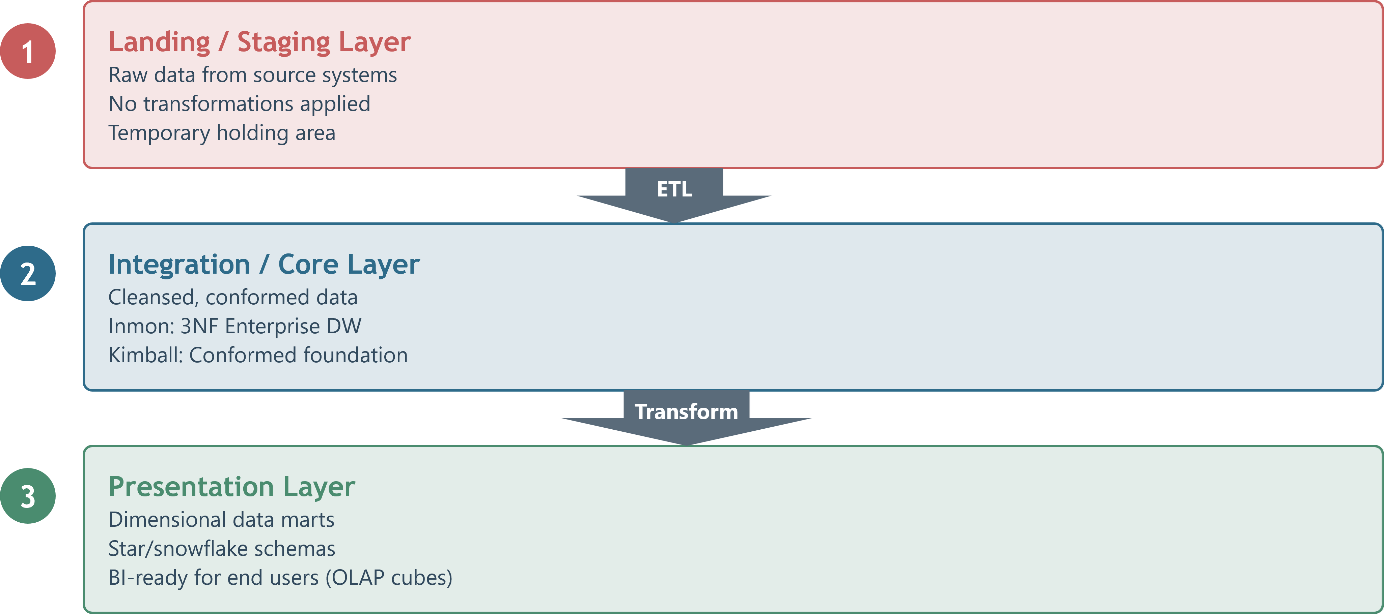
\includegraphics[width=0.85\linewidth]{slike/02/02-09.png}
    \caption{Трослојна референтна архитектура: прихватни слој (енг. staging), интеграциони слој (енг. integration) и презентациони слој (енг. presentation)}
    \label{fig:02-30}
\end{figure}

\textbf{\textit{Прихватни слој}} (енг. \textit{staging}) садржи сирове податке издвојене из изворних система. Подаци се учитавају суштински онако како су стигли — у изворним форматима, са изворним називима атрибута, са свим проблемима квалитета који су постојали на извору — и чувају се само онолико дуго колико захтева следећи циклус учитавања. Тај слој има две сврхе. Прво, изолује процес учитавања у складиште од изворних система: издвајање се може завршити у уском оперативном прозору, а спорије трансформације могу се независно извршавати над прихватном копијом без даљег оптерећења извора. Друго, обезбеђује контролну тачку за поновно покретање и опоравак: ако корак трансформације не успе, ETL процес се може наставити из прихватног слоја без поновног издвајања са извора.

\textbf{\textit{Интеграциони (или језгарни, енг. core)}} слој је место где се успоставља идентитет складишта. Подаци из прихватног слоја (енг. \textit{staging}) се чисте, стандардизују, усклађују са канонским форматима и помирују између извора; додељују се сурогатни кључеви (енг. \textit{surrogate keys}); примењује се SCD логика; спроводи се референтни интегритет (енг. \textit{referential integrity}). У Инмоновој методологији овај слој је enterprise 3NF складиште, јединствени извор истине из којег се изводе мартови. У Кимбаловој методологији овај слој је од почетка димензиони, са усаглашеним димензијама (енг. \textit{conformed dimensions}) и fact табелама изграђеним директно. У оба случаја, интеграциони слој је ниво на којем складиште задовољава Инмонове четири особине: тематски је оријентисано у својој организацији, интегрисано кроз изворе, неиспарљиво и временски варијантно.

\textbf{\textit{Презентациони слој}} (енг. \textit{presentation layer}) је оно што BI алати и крајњи корисници заправо упитују. Његове табеле су димензионе — звездасте или галаксијске шеме (енг. \textit{star} или \textit{galaxy schema}) — и подешене су за перформансе читања: агрегатне табеле (енг. \textit{aggregate tables}), материјализовани погледи (енг. \textit{materialized views}), колонарни индекси (енг. \textit{columnar indexes}) и, где се користе, OLAP коцке изграђене директно над димензионом шемом. Презентациони слој може бити засебна физичка структура (скуп мартова изведених из интеграционог слоја) или логички слој погледа над интеграционим слојем; избор је једна од дизајнерских одлука које разматра §2.2.4.6. Из перспективе корисника, презентациони слој јесте складиште: то је извор на који се контролна табла повезује и структура коју пивот табела чита.

Кроз сва три слоја протежу се две архитектонске дисциплине. Прва су метаподаци: свака табела, свака колона и свака трансформација документовани су у репозиторијуму метаподатака, тако да се порекло података (енг. \textbf{\textit{lineage}}) од извора преко прихватног, интеграционог и презентационог слоја може пратити. Порекло података је оно што складиште чини одбрањивим пред ревизорима, подложним отклањању грешака када је неки број погрешан и одрживим када се изворни системи мењају. Друга је праћење квалитета података: граница између прихватног и интеграционог слоја је природно место за примену правила квалитета (потпуност, јединственост, провере домена вредности), преусмеравање спорних редова у карантинску табелу (енг. \textbf{\textit{quarantine table}}) и упозоравање оперативног тима на систематске проблеме. §2.2.4.7.7 развија праксе квалитета података и профилисања кроз које се ове дисциплине операционализују.

\subsubsection{Хибридна пракса}
Већина организација значајне величине не спроводи ниједну методологију у чистом облику. Практични подразумевани образац најбоље је разумети као слојевиту референтну архитектуру из §2.2.4.5, у којој је сваком слоју додељена најприкладнија методологија. Тај образац комбинује предности оба приступа (Inmon et al., 2008; Kimball \& Ross, 2013). Интеграциони слој гради се у Инмоновом стилу: као нормализовани 3NF модел који обухвата интегрисано стање пословања, подржава могућност ревизије и отпоран је на промене у димензионим пројекцијама изграђеним изнад њега. Презентациони слој гради се у Кимбаловом стилу: као скуп димензионих мартова са усаглашеним димензијама, оптимизованих за употребу BI алата и за упите које корисник заиста извршава.

Хибридни образац разрешава централну напетост између ове две методологије. 3NF интеграциони слој гарантује доследност конструкцијом — сваки март је изведен из истог интегрисаног модела, па се дисциплина усаглашених димензија спроводи архитектонски, а не организационо. Истовремено, димензиони презентациони слој испоручује перформансе упита, читљивост шеме и компатибилност са BI алатима до којих је кориснику стало. Цена овог обрасца је то што се подаци материјализују два пута — једном у интеграционом слоју, једном у презентационом слоју — и ETL цевовод (енг. \textbf{\textit{ETL pipeline}}) мора да трансформише из 3NF у димензиони облик. У савременим изворно облачним складиштима тај трошак је подношљив, јер је складиштење јефтино, а димензиона пројекција може се имплементирати као погледи или као материјализације на захтев, а не као потпуно дуплиране табеле.

Хибридни образац такође прихвата даља архитектонска проширења која су ушла у праксу откако су канонске методологије успостављене. Data Vault 2.0 (Linstedt \& Olschimke, 2015), разматран у §2.2.4.8.1, природно стоји као алтернатива 3NF-у у интеграционом слоју: чува својства могућности ревизије која Инмонов приступ цени, уз боље прилагођавање честим променама шеме и паралелном учитавању него што то омогућава 3NF модел. Изворно облачна складишта (Snowflake, BigQuery, Redshift, Azure Synapse), разматрана у §2.2.4.8.3, мењају имплементациону технологију сваког слоја без промене саме слојевите структуре: складиштење и рачунарски ресурси су раздвојени, скалирање је еластично, а ELT образац из §2.2.4.7.6 помера тежак трансформациони рад са засебног ETL механизма на сопствени SQL механизам складишта. Архитектура језерског складишта (енг. \textit{lakehouse}) (Armbrust, Ghodsi, Xin, \& Zaharia, 2021), разматрана у §2.2.4.8.2, раствара границу између прихватног и интеграционог слоја тако што омогућава да сирови и курирани подаци коегзистирају у истом слоју складиштења са ACID семантиком. Ниједно од ових проширења не поништава слојевиту референтну архитектуру; свако мења физички изглед једног или више слојева, задржавајући њихову логичку улогу.

Општа поука је да методологија служи архитектонској потреби, а не обрнуто (Inmon et al., 2008). Студенту основних студија више користи разумевање слојевите архитектуре, методологија које се могу доделити сваком слоју и компромиса које свака таква додела подразумева, него третирање било Инмона (Inmon) било Кимбала (Kimball) као потпуног и самодовољног рецепта. Следећи пододељак прелази на интеграциони механизам који повезује слојеве — ETL или ELT цевовод — и разрађује га у дубини коју његов оперативни значај оправдава.

\subsubsection{ETL и ELT}
Екстракција, трансформација и учитавање (енг. \textit{extract-transform-load}, ETL) јесте процес којим се подаци крећу из изворних система преко прихватног слоја (енг. \textit{staging}) у интеграциони и презентациони слој складишта. То је истовремено оперативно најзначајнија и најпотцењенија компонента програма изградње складишта података: студије напора при имплементацији складишта редовно сврставају развој ETL-а на шездесет до осамдесет процената укупне цене пројекта (Kimball, Caserta, \& Mundy, 2008), а поузданост сваког извештаја и контролне табле које складиште служи зависи од исправности ETL цевовода (енг. \textit{ETL pipeline}) који је учитао основне табеле. Овај пододељак разматра сваку од три фазе редом, а затим испитује оркестрацију, разлику ETL/ELT и дисциплину квалитета података која се протеже кроз све фазе.

\textbf{\textit{Екстракција}} (енг. \textit{extraction}) јесте повезивање процеса учитавања у складиште са изворним системима. Извори су хетерогени: релационе базе података (SQL Server, Oracle, PostgreSQL), равне датотеке (енг. \textbf{\textit{flat files}}; CSV, fixed-width, Excel), пакетиране пословне апликације са сопственим интерфејсима за извоз, REST API-ји који враћају JSON, токови порука (енг. \textbf{\textit{message streams}}) и — у старијим организацијама — mainframe скупови података којима се приступа преко наменских конектора. Компонента издвајања у ETL цевоводу мора да прихвати сваки од ових типова извора и изолује остатак цевовода од њихових особености (Kimball et al., 2008).

Две стратегије екстракције су у уобичајеној употреби:

\begin{itemize}
  \item \textbf{\textit{Потпуно издвајање}} (енг. \textit{full extraction}) копира читав изворни скуп података при сваком покретању; једноставно је за имплементацију и отпорно на промене шеме изворног система, али се слабо скалира када су изворне табеле велике, а стопа промене мала.
  \item \textbf{\textit{Инкрементално издвајање}} (енг. \textit{incremental extraction}) копира само редове који су се променили од претходног покретања; то је доминантна стратегија у производним складиштима и оперативно место на коме заправо живи највећи део ETL сложености (Kimball et al., 2008).
\end{itemize}
Унутар инкременталног издвајања користе се три механизма за идентификацију промењених редова. Први су временски жигови као водене линије: изворна табела носи временски жиг последње измене, а свако издвајање тражи редове измењене након ознаке највише достигнуте вредности (енг. \textbf{\textit{high-water mark}}) из претходног покретања. Други је хватање промена у подацима (енг. \textbf{\textit{change-data capture}}, CDC): сам механизам изворне базе података бележи промене на нивоу реда (у PostgreSQL-у кроз логичку репликацију, у SQL Server-у кроз CDC функцију, у Oracle-у кроз GoldenGate), а процес издвајања конзумира тај лог. Трећи су заставице промене: апликација експлицитно означава редове као нове или измењене, а процес издвајања чисти заставицу након конзумирања.

CDC је пожељан за OLTP изворе великог обима јер бележи сваку промену на нивоу базе без измене апликације или ослањања на тачност временских жигова; водене линије су довољне за једноставније изворе где је обим умерен, а шема под контролом тима за складиште. Избор механизма није академски — он одређује шта ће складиште видети, а шта неће. Водена линија заснована на временском жигу пропушта брисања (обрисани ред нема преживели временски жиг по коме би се филтрирао); CDC их хвата. Заставица промене зависи од дисциплине апликације која временом може ослабити. Extraction дизајн мора бити усклађен са стварним понашањем изворног система, а усклађеност се мора поново преиспитати кад год се извор промени.

Четири оперативна ограничења обликују фазу издвајања. Прво, прозори доступности изворног система: производни OLTP системи не смеју бити успоравани издвајањем током радног времена, а издвајање мора бити завршено у дефинисаном ноћном или сатном прозору. Друго, права приступа и безбедност: није свака колона у извору одобрена за издвајање, а лично препознатљиви или регулисани подаци могу захтевати редакцију или псеудонимизацију на граници. Треће, неусаглашеност формата међу изворима: исти логички атрибут може стићи са различитим типовима, кодирањима, раздвајачима или представама null вредности из сваког извора, а компонента за издвајање мора сваки од њих да ухвати у облику који фаза трансформације може да обради. Четврто, мрежна латенција код удаљених и облачних извора: издвајање преко мреже ограничено је расположивом пропусношћу и толеранцијом на латенцију процеса који конзумира, што обоје ограничава колико агресивно инкрементално издвајање може бити постављено.

\textbf{\textit{Трансформација}} (енг. \textit{transformation}) је фаза у којој се издвојени подаци преобликују у канонски облик који складиште користи. Рад трансформације распада се на низ операција, од којих свака решава једну класу разлике између извора и одредишта (Kimball et al., 2008). Стандардни низ је прихватни слој (енг. \textit{staging}) → чишћење (енг. \textit{cleansing}) → стандардизација (енг. \textit{standardization}) → примена пословних правила (енг. \textit{application of business rules}) → генерисање кључева (енг. \textit{key generation}) → уклањање дупликата (енг. \textit{deduplication}) → припрема за интеграциони слој (енг. \textit{preparation for the integration layer}).

\textbf{\textit{Чишћење}} (енг. \textit{cleansing}) решава недостатке у изворним подацима. Null вредности морају бити обрађене — замењене подразумеваном вредношћу (нула, “непознато”, пословно дефинисано резервно решење), преусмерене у табелу одбијених редова (енг. \textbf{\textit{reject table}}) ради људског прегледа или учитане са колоном ознаке квалитета (енг. \textbf{\textit{quality flag}}) коју накнадни извештаји могу филтрирати. Неисправне вредности морају бити откривене и или исправљене према референтној листи или изоловане. Дупликатни редови морају бити идентификовани, било тачним поклапањем на кандидатском кључу или приближним поклапањем на атрибутима као што су имена и адресе тамо где се идентификатори изворних система не поклапају.

\textbf{\textit{Стандардизација}} (енг. \textit{standardization}) доводи сваку вредност у канонски облик. Датуми се претварају у ISO 8601 (“01/15/24”, “2024-01-15” и “Jan 15, 2024” сви постају 2024-01-15). Кодови држава се претварају у ISO 3166 (“US”, “USA” и “United States” сви постају US). Јединице мере се претварају у метрички систем (“kg”, “lbs” и “kilograms” сви постају kilograms у једној јединственој репрезентацији). Стандардизација је место где се интеграционо својство складишта — једнако значење подразумева једнаку репрезентацију, принцип наведен у §2.2.3.3 — оперативно спроводи.

\textbf{\textit{Примена пословних правила}} (енг. \textit{application of business rules}) је место на коме складиште спроводи логику организације за изведене мере и класификације. Израчунаване колоне — приход је количина пута цена, маржа је приход минус трошак, кашњење у данима је датум испоруке минус датум поруџбине — израчунавају се и чувају. Правила класификације — клијент високе вредности ако кумулативни приход прелази праг, касна испорука ако кашњење у данима прелази толеранцију — примењују се. Правила валидације — датум испоруке мора бити већи од датума поруџбине, клијент мора имати најмање осамнаест година — спроводе се, а редови који их крше преусмеравају се у карантинску табелу (енг. \textit{quarantine table}).

\textbf{\textit{Генерисање кључева}} (енг. \textit{key generation}) управља дисциплином сурогатног кључа (енг. \textit{surrogate key}) из §2.2.3.5.3. Природни кључеви (енг. \textit{natural keys}) из изворних система никада се не користе као примарни кључеви у складишту; уместо тога, сваки ред уметнут у димензиону табелу добија сурогатни кључ генерисан IDENTITY колоном или секвенцом, а сваки ред чињеница (енг. \textit{fact row}) повезује се са својим димензијама преко тих сурогатних кључева. Пресликавање кључева (енг. \textit{lookup}) које природни кључ из изворног система повезује са одговарајућим сурогатним кључем складишта јесте оперативно језгро учитавања димензија и место на коме се примењује SCD логика. Стандардни образац, извршен за сваки долазни изворни ред, гласи: пронађи природни кључ у димензионој табели; ако је ред нов, генериши нови сурогатни кључ и уметни; ако је ред непромењен, узми постојећи сурогатни кључ; ако је ред промењен, примени SCD стратегију декларисану за тај атрибут (затвори постојећи ред и уметни нови за тип 2, енг. \textit{Type 2}; препиши за тип 1, енг. \textit{Type 1}; ажурирај додатну колону за тип 3, енг. \textit{Type 3}); врати сурогатни кључ позиваоцу ради употребе у учитавању табеле чињеница (енг. \textit{fact-table loading}).

\textbf{\textit{Учитавање}} (енг. \textit{loading}) је уписивање трансформисаних података у складиште. Ова фаза има три тачке дисциплине: редослед учитавања, стратегију учитавања и обраду грешака.

Редослед учитавања ограничен је референтним интегритетом (енг. \textbf{\textit{referential integrity}}). Димензије морају бити учитане пре табела чињеница (енг. \textbf{\textit{fact tables}}) које их референцирају, јер су сурогатни кључеви додељени током учитавања димензија потребни учитавању табела чињеница ради попуњавања страних кључева. Стандардни редослед је прво табеле прихватног слоја (енг. \textbf{\textit{staging tables}}), затим димензионе табеле (са примењеном SCD логиком), па табеле чињеница (са пресликавањем сурогатних кључева, енг. \textbf{\textit{surrogate-key lookups}}, према управо учитаним димензијама). Обртање редоследа — учитавање чињеница пре димензија — производи редове чињеница чији страни кључеви још не постоје у димензионим табелама, нарушавајући референтни интегритет и кварећи сваки упит који спаја табелу чињеница и димензију. Ово ограничење је чврсто, а не саветодавно (Kimball et al., 2008).

Стратегија учитавања бира између потпуног поновног учитавања (енг. \textbf{\textit{full reload}}) и инкременталног дописивања и ажурирања (енг. \textbf{\textit{incremental upsert}}). Потпуно поновно учитавање празни циљну табелу и поново убацује сваки ред из прихватног слоја; једноставно је, отпорно на грешке у инкременталној логици и изводљиво за мале димензије, али брзо постаје неизводљиво за табеле чињеница са стотинама милиона редова. Инкрементално дописивање и ажурирање примењује MERGE операцију која убацује нове редове и ажурира промењене редове по примарном кључу; скалира се на веома велике табеле чињеница, али захтева дисциплину инкременталног издвајања описану на почетку овог одељка и осетљивије је на логичке грешке. У пракси се димензије типично потпуно поново учитавају (број њихових редова је довољно мали), а табеле чињеница се учитавају инкрементално.

Обрада грешака је место на коме се успоставља оперативна поузданост складишта. Одбачене датотеке (енг. \textbf{\textit{reject files}}) хватају редове који не прођу валидацију; карантинске табеле држе редове који пролазе валидацију али изазивају сумње у квалитет података; систем упозоравања (енг. \textbf{\textit{alerting}}) обавештава оперативни тим када стопе грешака пређу праг; стратегије враћања (енг. \textbf{\textit{rollback}}) омогућавају да се делимична учитавања врате када неки низводни корак не успе. Учитавање које откаже на пола пута може оставити складиште у недоследном стању — чињенице учитане уз делимично ажуриране димензије, или агрегате недоследне са основним детаљима — а опоравак из таквих стања скупљи је него њихово спречавање. Дисциплинован ETL цевовод третира свако учитавање као трансакциону целину: или се у потпуности заврши и потврди, или се враћа на претходно доследно стање.

\paragraph{Оркестрација и алати}
ETL цевовод није један програм већ граф зависних задатака: издвајање из сваког извора, кораци трансформације у низу, учитавања димензија, учитавања чињеница, освежавања агрегата и накнадна обавештења. Оркестрација је дисциплина заказивања ових задатака, спровођења њихових зависности, праћења њиховог извршења и опоравка од неуспеха. Четири појма оркестрације су стандардна (Kimball et al., 2008). Распоређивање (енг. \textbf{\textit{scheduling}}) одређује када се цевоводи извршавају — ноћно, сваки сат, на догађајне окидаче или као непрекидни токови. Управљање зависностима осигурава да се низводни задатак покрене тек након што сваки узводни задатак од кога зависи успешно заврши; ако било који узводни задатак не успе, зависни задаци се задржавају док се неуспех не разреши. Праћење (енг. \textbf{\textit{monitoring}}) бележи логове извршења, бројеве редова у свакој фази, трајања и стопе грешака, и излаже их и за оперативно упозоравање и за дугорочно планирање капацитета. Опоравак (енг. \textbf{\textit{recovery}}) дефинише логику поновног покретања: цевовод који откаже на пола пута мора бити могуће поново покренути из контролне тачке, а не од почетка, и оркестратор (енг. \textbf{\textit{orchestrator}}) мора да спроведе идемпотентност (енг. \textbf{\textit{idempotency}}) тако да поново покренути задатак не дуплира рад свог ранијег покушаја.

Четири породице алата доминирају оркестрационим пејзажом. SQL Server Integration Services (SSIS) је Microsoft-ова традиционална ETL платформа, тесно интегрисана са SQL Server екосистемом и широко примењена у организацијама стандардизованим на Microsoft технологији. Apache Airflow је оркестратор отвореног кода (енг. \textbf{\textit{open-source orchestrator}}) најшире усвојен у новим пројектима: цевоводи се дефинишу као Python усмерени ациклични графови (енг. \textbf{\textit{directed acyclic graphs}}, DAGs), инфраструктура за заказивање и праћење је зрела, а екосистем изворних конектора је велик. Talend нуди интеграциону платформу за велике организације, са графичким дизајнером цевовода и широком библиотеком конектора. Tableau Prep пружа уже фокусиран алат оријентисан ка припреми података коју воде аналитичари, а не ка ETL-у на нивоу предузећа. Избор између њих мање је вођен поређењем функционалности, а више постојећим технолошким стеком организације и профилом вештина тима који ће управљати цевоводом.

\paragraph{Пример од почетка до краја}
Дисциплина претходних пододељака постаје опипљива када се прати један продајни запис од извора до табеле чињеница. Пример испод репродукује разрађени цевовод из изворне презентације и репрезентативан је за оно што ETL цевовод мора да уради за један ред FACT\_SALES (Слика~\ref{fig:02-31}).

\begin{figure}[h]
    \centering
    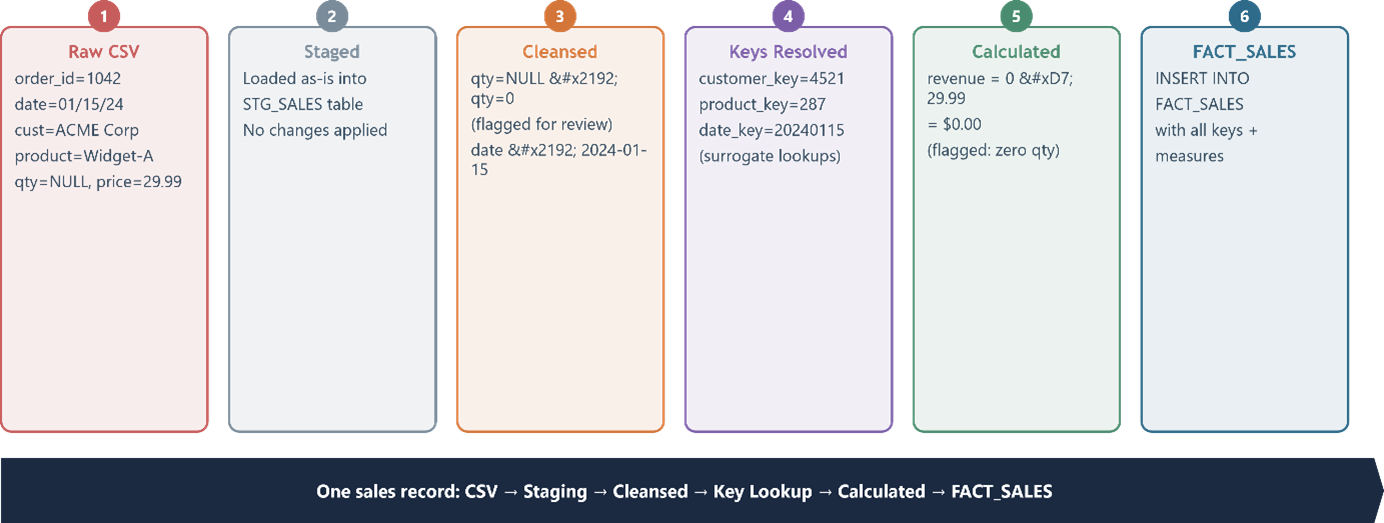
\includegraphics[width=0.85\linewidth]{slike/02/02-11.png}
    \caption{ETL цевовод (енг. ETL pipeline) од почетка до краја: један продајни запис праћен од сировог CSV-а до FACT\_SALES}
    \label{fig:02-31}
\end{figure}

CSV фајл из система за управљање поруџбинама стиже у прихватну област (енг. \textit{staging area}) са редом који садржи \texttt{order\_id = 1042}, \texttt{date = „01/15/24”}, \texttt{cust = „ACME Corp”}, \texttt{product = „Widget-A”}, \texttt{qty = NULL}, \texttt{price = 29,99}. Ред се учитава у прихватну табелу \texttt{STG\_SALES} тачно онако како је примљен, без примењене трансформације. У том тренутку складиште држи ред у изворном облику: сваки недостатак у изворној вредности очуван је дословно како би накнадно чишћење (енг. \textbf{\textit{cleansing}}) имало све доказе потребне за деловање.

Чишћење претвара поље датума из US формата “01/15/24” у канонски ISO 8601 облик 2024-01-15. Недостајућа количина (\texttt{NULL}) се замењује нулом и ред се означава за преглед у колони квалитета података; алтернатива — потпуно одбацивање реда — резервисана је за случајеве у којима је \texttt{NULL} структурно неважећи, а не поправљив недостатак. Даље промене се не примењују: називи купца и производа остају у облику природног кључа (енг. \textit{natural key}), чекајући пресликавање сурогатног кључа (енг. \textit{surrogate-key lookup}) у следећем кораку.

Разрешење сурогатног кључа тражи сваки природни кључ у одговарајућој димензионој табели. Купац “ACME Corp” налази се у \texttt{DIM\_CUSTOMER} и враћа \texttt{customer\_sk = 4521} (његову текућу верзију типа 2, енг. \textit{Type 2}). Производ “Widget-A” налази се у \texttt{DIM\_PRODUCT} и враћа \texttt{product\_sk = 287}. Очишћени датум 2024-01-15 налази се у \texttt{DIM\_DATE} и враћа \texttt{date\_sk = 20240115}. Да се неки од природних кључева није поклопио, ред би био преусмерен у карантинску табелу; у овом примеру сва три се уредно разреше.

\textbf{\textit{Примена пословних правила}} (енг. \textit{application of business rules}) израчунава изведене мере које табела чињеница захтева. Приход се израчунава као количина пута цена: у овом случају, нула пута 29,99 једнако је 0,00 RSD. Ред се означава у посебној колони да покаже да вредност нултог прихода потиче од недостатка у пољу количине, а не од стварне трансакције са нултим приходом. Ова разлика је важна за накнадно извештавање: контролна табла која агрегира приход треба да укључи ред као нулу (како би се укупни износи усагласили), али треба и да прикаже број ознака недостатака како би проблеми квалитета података били видљиви.

Завршни корак убацује ред у FACT\_SALES који носи три сурогатна кључа (енг. \textit{surrogate keys}), очишћене и израчунате мере (qty = 0, price = 29,99, revenue = 0,00) и ознаке квалитета података. Ред је сада део интегрисаног, временски обележеног записника продајног процеса заснованог на сурогатним кључевима. Упит контролне табле који агрегира приход по купцу и месецу дохватиће овај ред преко његових date\_sk и customer\_sk и комбиновати га са сваком другом продајом тог периода; ред ће се моћи ускладити са својим изворним CSV-ом преко order\_id, који је очуван као дегенерисана димензија на fact табели.

\paragraph{ETL насупрот ELT}
До отприлике 2015. године стандардни образац је недвосмислено био ETL: подаци су се издвајали из извора, трансформисали засебним механизмом (SSIS, Informatica, Talend) и учитавали у складиште већ у свом коначном облику. Механизам трансформације био је засебан део инфраструктуре са сопственим рачунарским ресурсима и сопственим карактеристикама скалирања. Овај образац је добро одговарао локално постављеним складиштима (енг. \textbf{\textit{on-premises}} warehouses) са ограниченим рачунарским капацитетом, где је резервисање ресурса складишта за радно оптерећење упита и измештање трансформације у засебан механизам било архитектонска нужност.

Пораст изворно облачних складишта — Snowflake, BigQuery, Redshift, Azure Synapse — променио је ограничење. Облачна складишта раздвајају складиштење од рачунарских ресурса и нуде еластичне ресурсе који се наплаћују по упиту (енг. \textbf{\textit{pay-per-query}}) и који се на захтев скалирају на огромна оптерећења. У овом режиму трансформација се може изводити унутар самог складишта употребом његовог сопственог SQL механизма, при чему се сирови подаци прво учитавају у складиште, а трансформације примењују као SQL искази над учитаним табелама. Тај образац назива се ELT — издвоји, учитај, трансформиши (енг. \textit{extract, load, transform}). Подаци се учитавају у складиште у сировом или скоро сировом облику; трансформациони рад се изражава као SQL, често слојевито преко алата као што је dbt који додаје управљање верзијама (енг. \textit{version control}), тестирање (енг. \textit{testing}) и управљање зависностима (енг. \textit{dependency management}); еластични рачунарски ресурси складишта скалирају се и на трансформационо и на упитно оптерећење. Помак ка ELT-у био је једна од најзначајнијих архитектонских промена последње деценије и у великој мери је демократизовао изградњу складишта, уклањањем потребе за посебним ETL механизмом и специјализованим вештинама потребним за његово одржавање.

Избор између ETL-а и ELT-а сада је питање усклађености, а не могућности. ELT је природан избор за изворно облачна складишта са еластичним рачунарским ресурсима, за организације које преферирају SQL-засновану трансформациону логику уместо цевовода графичких алата и за пројекте где је време до прве вредности важније од изолације инфраструктуре. ETL остаје прави избор за осетљиве податке који морају бити очишћени пре него што буду трајно уписани у складиште, јер сами сирови, неочишћени подаци могу бити регулаторни или безбедносни проблем, за локално постављена складишта где су рачунарски ресурси ограничени и за организације чије је постојеће улагање у ETL алате велико. dbt — SQL-first оквир за трансформацију који је сада фактички стандард (енг. \textbf{\textit{de facto standard}}) за ELT цевоводе на облачним складиштима — био је главни убрзивач усвајања ELT-а отприлике од 2018. године.

\paragraph{Квалитет података и профилисање}
Квалитет података је дисциплина која осигурава да складиште испоручује тачне, потпуне, доследне и благовремене податке својим корисницима; она се спроводи кроз профилисање, правила квалитета и континуирано праћење (Kimball et al., 2008). Профилисање је систематско испитивање изворних података пре него што буду моделовани или учитани: потпуност колона (удео null вредности), расподела вредности (табеле фреквенција за категоријалне атрибуте, сумарне статистике за нумеричке атрибуте), откривање образаца (усаглашеност са регуларним изразима за поља као што су email и поштански број), анализа јединствености (да ли су кандидатски кључеви заиста јединствени) и провере доследности између извора (да ли исти купац у два система носи атрибуте који се могу помирити). Аргумент за профилисање, изречен без увијања од стране практичара који су га развили, јесте да складиште не може бити исправно моделовано док се не разуме стварни облик његових изворних података — а стварни облик ретко је оно што тврди изворна документација.

Правила квалитета, примењена током фаза чишћења и валидације у трансформацији, кодирају очекивања организације о њеним подацима. Правила се крећу од једноставних (старост купца мора бити позитивна, код државе мора постојати у ISO 3166) до сложених (уплата мора да се помири са отвореним рачуном у оквиру толеранције). Свако правило има дефинисан одговор када је прекршено: одбаци ред, преусмери га у карантин, учитај га са ознаком квалитета (енг. \textbf{\textit{quality flag}}) или упозори оператера. Избор одговора сам по себи је одлука квалитета података и бележи се у метаподацима складишта.

\textbf{\textit{Праћење}} (енг. \textit{monitoring}) затвара петљу. Правила квалитета која пролазе у време моделовања могу почети да отказују како се изворни системи развијају; профилисање које је било тачно пре годину дана можда више не одражава податке које извор данас производи. Зрела пракса управљања складиштем непрекидно извршава правила квалитета, прати стопе пролаза кроз време и упозорава оперативни тим када стопе падну испод прага или када новоуведена правила открију раније немоделоване недостатке. Ово је оперативна манифестација принципа да квалитет није својство једног учитавања, већ својство складишта као непрекидно еволуирајућег система.

\subsubsection{Савремени правци}
Методологије Инмона и Кимбала успостављене су између касних 1980-их и раних 2000-их, када су складишта била локално постављена (енг. \textbf{\textit{on-premises}}), рачунарски ресурси и складиштење били тесно повезани, а изворни системи бројали десетине. Архитектонски пејзаж се од тада значајно променио. Три развоја ушла су у праксу током последње деценије и сада су стандардни делови сваке савремене расправе: Data Vault 2.0 као алтернативни образац моделовања интеграционог слоја, језерско складиште (енг. \textbf{\textit{lakehouse}}) као архитектонска фузија језера података (енг. \textbf{\textit{data lake}}) и складишта, и изворно облачна складишта (енг. \textbf{\textit{cloud-native warehouses}}) као доминантна платформа за распоређивање. Овај пододељак разматра сваки од њих у сажетом облику, уз кратак преглед даљих трендова — интеграције AI/ML-а, data mesh-а и аналитике токова података — који обликују пејзаж складишта крајем 2020-их.

\paragraph{Data Vault 2.0}
Data Vault 2.0, који је увео Ден Линстед (Dan Linstedt) почетком 2000-их и кодификован у раду Линстеда и Олшимајкеа (Linstedt \& Olschimke, 2015), алтернативни је образац моделовања интеграционог слоја складишта. Док Инмонов 3NF модел хвата пословна правила у шеми, а Кимбалов димензиони модел их хвата у усаглашеним димензијама, Data Vault у потпуности раздваја структурне и дескриптивне бриге шеме. Модел чине три типа табела: чворишта (енг. \textit{hubs}) држе јединствене пословне кључеве за сваки субјект (купац, производ, поруџбина); везе (енг. \textit{links}) држе односе између чворишта; а сателити (енг. \textit{satellites}) држе описне атрибуте који описују чвориште или везу, при чему је сваки сателит означен временом учитавања тако да се историја акумулира додавањем редова, а не ажурирањем постојећих.

Посебна својства овог обрасца следе из тог раздвајања. Могућност ревизије је структурна: сваки ред носи изворни систем и време учитавања, а свако историјско стање сваког ентитета може се реконструисати избором satellite табела за одређени тренутак у времену. Еволуција шеме је локална: додавање атрибута субјекту значи додавање satellite табеле, а не модификацију постојеће табеле; додавање новог извора значи додавање satellite табеле која бележи виђење тог извора, без нарушавања постојећих satellite табела. Паралелно учитавање је подржано јер се hubs, links и satellites могу учитавати независно — не постоје зависности страних кључева које би на интеграционом слоју наметале секвенцијални редослед учитавања (Linstedt \& Olschimke, 2015). Цена је у томе што Data Vault није модел окренут кориснику: BI алати га не могу директно упитивати уз употребљиве перформансе, и димензиони презентациони слој мора бити изграђен изнад њега, типично као погледи или материјализоване пројекције. Тај образац је стога допуна димензионом моделу, а не његова замена, и природно стоји као интеграциони слој у слојевитој архитектури из §2.2.4.5, са мартовима у Кимбаловом стилу као презентационим слојем.

Data Vault најбоље одговара организацијама које интегришу много извора, суочавају се са честим променама шеме и послују у регулаторним режимима који захтевају снажну могућност ревизије — финансијске услуге, здравство, регулисана комунална предузећа. Претерано је спецификован за организације са стабилним шемама и мало извора, где његов оперативни трошак превазилази његове користи.

\paragraph{Језерско складиште}
\textbf{\textit{Језерско складиште}} (енг. \textit{lakehouse}), које су увели Армбраст, Годси, Син и Захарија (Armbrust, Ghodsi, Xin, \& Zaharia, 2021), представља архитектонску фузију два ранија обрасца (Слика~\ref{fig:02-32}): језера података (енг. \textbf{\textit{data lake}}), односно јефтиног складиштења сирових, неструктурираних и полуструктурираних података по принципу schema-on-read, и складишта података (енг. \textbf{\textit{data warehouse}}), односно курираног аналитичког складишта које примењује schema-on-write и ACID гаранције. Језерско складиште држи сирове, полуструктуриране и структуриране податке у једном слоју складиштења — типично у облачном објектном складишту (енг. \textbf{\textit{cloud object storage}}) као што су Amazon S3 или Azure Data Lake Storage — и надграђује их отвореним форматом табеле (Delta Lake, Apache Iceberg или Apache Hudi) који обезбеђује ACID трансакције, спровођење шеме и путовање кроз време (енг. \textbf{\textit{time travel}}) над основним складиштем објеката (енг. \textbf{\textit{object store}}). Резултат је јединствена платформа која подржава SQL аналитику, машинско учење и анализу токова података (енг. \textbf{\textit{streaming}}) над истим физичким подацима, елиминишући засебан ETL цевовод који је традиционално премештао куриране податке из језера у складиште.

\begin{figure}[h]
    \centering
    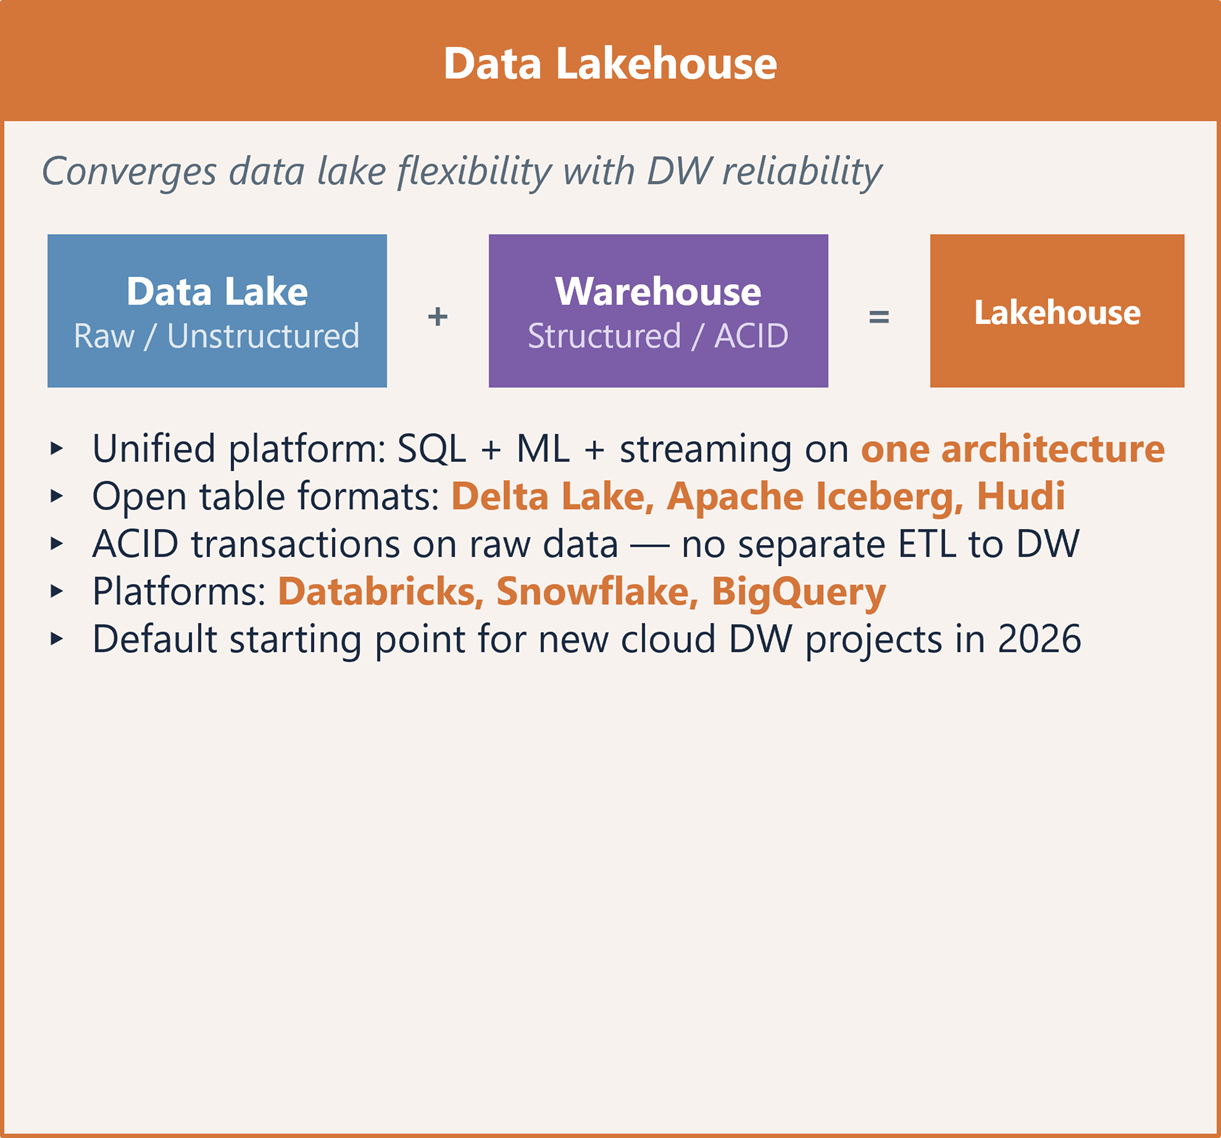
\includegraphics[width=0.85\linewidth]{slike/02/02-28.png}
    \caption{Архитектура језерског складишта (енг. lakehouse): флексибилност језера података (енг. data lake) комбинована са ACID гаранцијама складишта кроз отворене формате табела}
    \label{fig:02-32}
\end{figure}

Две последице ове архитектуре посебно су релевантне за ово потпоглавље. Прво, граница између прихватног (енг. \textbf{\textit{staging}}) и интеграционог слоја из §2.2.4.5 се раствара: сирови и курирани подаци коегзистирају у истом слоју складиштења, разликовани трансакционим гаранцијама формата табеле, а не физичким раздвајањем. Друго, платформа подржава аналитичка оптерећења (SQL упити, BI алати) и оптерећења машинског учења (обука модела, обликовање карактеристика, енг. \textbf{\textit{feature engineering}}) без потребе да се подаци премештају између система, што поједностављује управљање и смањује кашњење између доласка података и њихове накнадне употребе. Databricks је платформа која се најтешње повезује са lakehouse обрасцем, али Snowflake, BigQuery и друга облачна складишта усвојила су lakehouse могућности као део своје основне понуде, и овај образац је ефективно постао подразумевана полазна тачка за нове изворно облачне пројекте складишта (Armbrust et al., 2021).

\paragraph{Изворно облачна складишта}
Cloud-native складишта — Snowflake, Google BigQuery, Amazon Redshift и Microsoft Azure Synapse Analytics — деле архитектонски принцип који их разликује од on-premises складишта: складиштење и рачунарски ресурси су раздвојени, скалирају се независно и наплаћују независно. Складиштење се држи у cloud object storage-у, рачунарски ресурси се по потреби обезбеђују као скуп еластичних virtual warehouses, а упит коме треба више ресурса добија их током трајања упита и ослобађа по завршетку. Овај образац омогућава serverless и pay-per-query оперативне моделе у којима је складиште, из перспективе корисника, једноставно доступно уместо унапред обезбеђено.

Архитектонско раздвајање складиштења од рачунарских ресурса преобликовало је економику складиштења. Цена чувања историјских података пала је на ниво на коме је неиспарљивост — особина коју складиште и постоји да спроведе — постала практично бесплатна, уклањајући један од историјских притисака ка агресивној агрегацији и архивирању података. Еластичност рачунарских ресурса померила је архитектонски баланс ка ELT-у (§2.2.4.7.6), јер сопствени SQL механизам складишта може да апсорбује трансформациона оптерећења која би раније захтевала засебну ETL платформу. Аналитичари индустрије извештавају да је тржиште cloud-native складишта порасло са приближно тридесет осам милијарди америчких долара у 2025. на пројектованих седамдесет милијарди до 2029, што одражава прелазак складишта из специјализоване инфраструктурне компоненте у подразумевану cloud услугу.

\paragraph{Даљи трендови}
Три даља развоја обликују пејзаж складишта крајем 2020-их и заслужују кратак осврт. AI/ML интеграција помера складиште од пасивне платформе за извештавање ка активном аналитичком окружењу у коме се модели обучавају, упити оптимизују, а аномалије детектују компонентама машинског учења уграђеним у само складиште. Интерфејси природног језика, у којима корисници постављају питања на енглеском, а систем генерише SQL, прешли су пут од истраживачких прототипова до комерцијалних производа. Gartner је пројектовао да ће до 2026. већина аналитичких оптерећења у неком облику зависити од AI/ML компоненти.

Data mesh, који је увела Dehghani (2022), образац је управљања и власништва, а не технологија. Он предлаже да одговорност за аналитичке производе података (енг. \textbf{\textit{data products}}) буде децентрализована на пословне домене који податке производе — продаја поседује свој производ података, финансије поседују свој — уз федеративни оквир управљања који обезбеђује интероперабилност. Овај образац је одговор на ограничења скалирања централних тимова за складишта у великим организацијама и није замена за архитектонске обрасце овог потпоглавља; он је питање ко поседује и управља складиштем, а не шта складиште јесте.

\textbf{\textit{Аналитика токова података}} (енг. \textit{streaming analytics}), подржана платформама као што су Apache Kafka и њиховим облачним еквивалентима (Amazon Kinesis, Google Pub/Sub), смањује кашњење између доласка података и аналитичке доступности са сати или дана, колико траје типичан пакетни прозор традиционалног складишта, на секунде. Овај образац је важан за случајеве употребе као што су детекција превара, оперативно праћење и персонализација у реалном времену, у којима вредност одговора брзо опада с временом. Архитектонска интеграција токова података са складиштем остаје активно поље пројектовања, са обрасцима као што су lambda и kappa архитектуре, материјализовани погледи над токовима (енг. \textbf{\textit{materialized streaming views}}) и инкрементална материјализација (енг. \textbf{\textit{incremental materialization}}) преко алата као што је dbt, који нуде различите компромисе између латенције и доследности.

Ови развоји не поништавају архитектонске темеље постављене у §§2.2.3 и 2.2.4. Складиште остаје тематски оријентисано, интегрисано, неиспарљиво и временски варијантно; димензионо моделовање остаје доминантан образац за слој окренут кориснику; ETL или ELT остаје интеграциони механизам. Оно што се променило јесу имплементациона технологија, модел распоређивања и границе између складишта и суседних платформи — а оно што је остало јесте архитектонско расуђивање које стоји у основи улоге складишта као подршке управљачким одлукама.

\subsection{Подршка извештавању}
Одељци 2.1.1–2.1.10 увели су четири технике корисничког слоја (енг. \textbf{\textit{front end}}) — визуализацију (§§2.1.1–2.1.6), израду контролних табли (§2.1.9), приповедање помоћу података (§2.1.7) и пивот табелу — без прецизирања на чему су оне засноване. Ово потпоглавље је обезбедило недостајући позадински слој (енг. \textbf{\textit{back end}}). Завршни одељак прати свако архитектонско својство складишта до одговарајуће способности корисничког слоја, чини те зависности експлицитним и припрема читаоца да у сваком наредном BI артефакту на који наиђе препозна које својство складишта обавља тај посао.

\subsubsection{Од својстава складишта до аналитичких способности}
\textbf{\textit{Усаглашене димензије}} (енг. \textit{conformed dimensions}) омогућавају доследне контролне табле. Контролна табла која на једном екрану приказује приход од продаје, маркетиншку потрошњу и тикете корисничке подршке има смисла само ако су та три броја упоредива — рашчлањена по истим временским периодима, истим регионима и истим сегментима купаца. Усаглашене димензије, интеграциони механизам из §2.2.4.3, архитектонско су средство које ово поређење чини могућим: свака табела чињеница придружује се истој DIM\_DATE, истој DIM\_GEOGRAPHY и истој DIM\_CUSTOMER, са атрибутима дефинисаним и управљаним идентично кроз мартове. Контролна табла коју корисник гради у Power BI-ју или Tableau-у ради зато што је складиште испод ње већ обавило посао усаглашавања (енг. \textit{conformance}).

Неиспарљивост и временска варијантност омогућавају приповедање са историјском дубином. Наратив који објашњава како је пословање стигло у свој тренутни положај захтева податке о сваком претходном положају — кварталне путање прихода, поређења из године у годину, кохорте купаца какве су биле у тренутку када је свака кохорта стечена. Образац дописивања без преписивања (енг. \textbf{\textit{append-only}}) из §2.2.3.4 задржава свако стање кроз које је пословање прошло; дисциплина временске варијантности из §2.2.3.5 организује та стања тако да се могу упитивати по датуму. Способност приповедача да покаже „шта се променило” јесте неиспарљивост и временска варијантност складишта учињена видљивом.

Претходно агрегиране коцке омогућавају интерактивне пивот табеле и продубљивање увида (енг. \textbf{\textit{drill-down}}). Пивот табела је аналитичарев инструмент за сечење мера кроз димензије; §2.2.3.7 дао је формални приказ OLAP коцке као њене структуре података. Интерактивна одзивност коју корисник доживљава — превуците димензију у област редова и посматрајте како се унакрсна табела преобликује, проширите хијерархију и гледајте како се месеци отварају унутар године — јесте рад претходно агрегираних вредности и индексираних претрага (енг. \textbf{\textit{lookup}}) коцке, над унапред израчунатим ћелијама, а не над скенирањем табела чињеница.

Тематски оријентисана интеграција омогућава једну верзију истине кроз визуализације. Финансијска контролна табла која извештава о кварталном приходу и продајна контролна табла која извештава о истом приходу морају показати исти број; прича која цитира неку цифру мора се ускладити са контролним таблама које је приказују; пивот табела коју аналитичар гради за ad hoc анализу мора бити сагласна са оба. Тематска оријентација (§2.2.3.2) и интеграција (§2.2.3.3) чине ово поклапање структурним, а не случајним: сваки артефакт црпи из истог усклађеног, интегрисаног и управљаног приказа пословања, а доследност корисничког слоја (енг. \textbf{\textit{front end}}) јесте, на крају, дисциплина интеграције позадинског слоја (енг. \textbf{\textit{back end}}) учињена видљивом на корисниковом екрану.

\section{Литература}
Armbrust, M., Ghodsi, A., Xin, R., \& Zaharia, M. (2021). Lakehouse: A new generation of open platforms that unify data warehousing and advanced analytics. In Proceedings of the 11th Conference on Innovative Data Systems Research (CIDR).

Becker, R. A., \& Cleveland, W. S. (1987). Brushing scatterplots. Technometrics, 29(2), 127–142.

Bostock, M., Ogievetsky, V., \& Heer, J. (2011). D³ data-driven documents. IEEE Transactions on Visualization and Computer Graphics, 17(12), 2301–2309. https://doi.org/10.1109/TVCG.2011.185

Box, G. E. P., Jenkins, G. M., Reinsel, G. C., \& Ljung, G. M. (2015). Time series analysis: Forecasting and control (5th ed.). Wiley.

Cairo, A. (2016). The truthful art: Data, charts, and maps for communication. New Riders.

Card, S. K., Mackinlay, J. D., \& Shneiderman, B. (1999). Readings in information visualization: Using vision to think. Morgan Kaufmann.

Chaudhuri, S., \& Dayal, U. (1997). An overview of data warehousing and OLAP technology. ACM SIGMOD Record, 26(1), 65–74. https://doi.org/10.1145/248603.248616

Chen, H., Chiang, R. H. L., \& Storey, V. C. (2012). Business intelligence and analytics: From big data to big impact. MIS Quarterly, 36(4), 1165–1188.

Cleveland, W. S. (1993). Visualizing data. Hobart Press.

Cleveland, W. S., \& McGill, R. (1984). Graphical perception: Theory, experimentation, and application to the development of graphical methods. Journal of the American Statistical Association, 79(387), 531–554.

Codd, E. F. (1970). A relational model of data for large shared data banks. Communications of the ACM, 13(6), 377–387. https://doi.org/10.1145/362384.362685

Codd, E. F., Codd, S. B., \& Salley, C. T. (1993). Providing OLAP to user-analysts: An IT mandate. Codd \& Associates.

Cressie, N. (1993). Statistics for spatial data. Wiley.

Davenport, T. H., \& Harris, J. G. (2007). Competing on analytics: The new science of winning. Harvard Business School Press.

Dehghani, Z. (2022). Data mesh: Delivering data-driven value at scale. O’Reilly Media.

Eckerson, W. W. (2010). Performance dashboards: Measuring, monitoring, and managing your business (2nd ed.). Wiley.

Few, S. (2006). Information dashboard design: The effective visual communication of data. O’Reilly Media.

Few, S. (2009). Now you see it: Simple visualization techniques for quantitative analysis. Analytics Press.

Few, S. (2012). Show me the numbers: Designing tables and graphs to enlighten (2nd ed.). Analytics Press.

Few, S. (2013). Information dashboard design: Displaying data for at-a-glance monitoring (2nd ed.). Analytics Press.

Gelman, A., \& Hill, J. (2007). Data analysis using regression and multilevel/hierarchical models. Cambridge University Press.

Golfarelli, M., \& Rizzi, S. (2009). Data warehouse design: Modern principles and methodologies. McGraw-Hill.

Härder, T., \& Reuter, A. (1983). Principles of transaction-oriented database recovery. ACM Computing Surveys, 15(4), 287–317. https://doi.org/10.1145/289.291

Hastie, T., Tibshirani, R., \& Friedman, J. (2009). The elements of statistical learning: Data mining, inference, and prediction (2nd ed.). Springer.

Heer, J., \& Shneiderman, B. (2012). Interactive dynamics for visual analysis. Communications of the ACM, 55(4), 45–54. https://doi.org/10.1145/2133806.2133821

Inmon, W. H. (2005). Building the data warehouse (4th ed.). Wiley.

Inmon, W. H., Strauss, D., \& Neushloss, G. (2008). DW 2.0: The architecture for the next generation of data warehousing. Morgan Kaufmann.

James, G., Witten, D., Hastie, T., \& Tibshirani, R. (2021). An introduction to statistical learning (2nd ed.). Springer.

Kaplan, R. S., \& Norton, D. P. (1996). The balanced scorecard: Translating strategy into action. Harvard Business School Press.

Keim, D. A., Andrienko, G., Fekete, J.-D., Görg, C., Kohlhammer, J., \& Melançon, G. (2010). Visual analytics: Definition, process, and challenges. In A. Kerren et al. (Eds.), Information visualization (pp. 154–175). Springer.

Keim, D. A., Mansmann, F., Schneidewind, J., Thomas, J., \& Ziegler, H. (2008). Visual analytics: Scope and challenges. In Visual data mining (pp. 76–90). Springer. https://doi.org/10.1007/978-3-540-71080-6\_6

Kimball, R., Caserta, J., \& Mundy, J. (2008). The data warehouse ETL toolkit: Practical techniques for extracting, cleaning, conforming, and delivering data. Wiley.

Kimball, R., \& Ross, M. (2013). The data warehouse toolkit: The definitive guide to dimensional modeling (3rd ed.). Wiley.

Kimball, R., Ross, M., Thornthwaite, W., Mundy, J., \& Becker, B. (2008). The data warehouse lifecycle toolkit (2nd ed.). Wiley.

Knaflic, C. N. (2015). Storytelling with data: A data visualization guide for business professionals. Wiley.

Knaflic, C. N. (2020). Storytelling with data: Let’s practice! Wiley.

Kosara, R., \& Mackinlay, J. (2013). Storytelling: The next step for visualization. Computer, 46(5), 44–50. https://doi.org/10.1109/MC.2013.36

Linstedt, D., \& Olschimke, M. (2015). Building a scalable data warehouse with Data Vault 2.0. Morgan Kaufmann.

Marr, B. (2016). Big data in practice: How 45 successful companies used big data analytics to deliver extraordinary results. Wiley.

Munzner, T. (2014). Visualization analysis and design. CRC Press.

Newman, M. E. J. (2018). Networks (2nd ed.). Oxford University Press.

Rahm, E., \& Bernstein, P. A. (2001). A survey of approaches to automatic schema matching. The VLDB Journal, 10(4), 334–350. https://doi.org/10.1007/s007780100057

Sarikaya, A., Correll, M., Bartram, L., Tory, M., \& Fisher, D. (2019). What do we talk about when we talk about dashboards? IEEE Transactions on Visualization and Computer Graphics, 25(1), 682–692.

Satyanarayan, A., Moritz, D., Wongsuphasawat, K., \& Heer, J. (2017). Vega-Lite: A grammar of interactive graphics. IEEE Transactions on Visualization and Computer Graphics, 23(1), 341–350.

Segel, E., \& Heer, J. (2010). Narrative visualization: Telling stories with data. IEEE Transactions on Visualization and Computer Graphics, 16(6), 1139–1148. https://doi.org/10.1109/TVCG.2010.179

Sharda, R., Delen, D., \& Turban, E. (2020). Business intelligence, analytics, and data science: A managerial perspective (4th ed.). Pearson.

Sheth, A. P., \& Larson, J. A. (1990). Federated database systems for managing distributed, heterogeneous, and autonomous databases. ACM Computing Surveys, 22(3), 183–236. https://doi.org/10.1145/96602.96604

Shneiderman, B. (1996). The eyes have it: A task by data type taxonomy for information visualizations. In Proceedings of the IEEE Symposium on Visual Languages (pp. 336–343). IEEE.

Slocum, T. A., McMaster, R. B., Kessler, F. C., \& Howard, H. H. (2009). Thematic cartography and geovisualization (3rd ed.). Pearson.

Stevens, S. S. (1946). On the theory of scales of measurement. Science, 103(2684), 677–680.

Tufte, E. R. (1990). Envisioning information. Graphics Press.

Tufte, E. R. (2001). The visual display of quantitative information (2nd ed.). Graphics Press.

Tukey, J. W. (1977). Exploratory data analysis. Addison-Wesley.

Ware, C. (2013). Information visualization: Perception for design (3rd ed.). Morgan Kaufmann.

Wickham, H., \& Grolemund, G. (2017). R for data science. O’Reilly Media.

Wilke, C. O. (2019). Fundamentals of data visualization. O’Reilly Media.

Wilkinson, L. (2005). The grammar of graphics (2nd ed.). Springer.
